\chapter{SUSY searches in Hadronic Final States}
\label{chap:SUSYsearches}

In this chapter a model independent search for \ac{SUSY} in hadronic final states with $\met$ using the $\alphat$ variable and b-quark multiplicity is introduced and described in detail. The results presented are based on a data sample of pp collisions collected in 2012 at $\com =$8 \TeV, corresponding to an integrate luminosity of 11.7$\pm$0.5 fb$^{-1}$.

The kinematic variable $\alphat$ is motivated as a variable to provide strong rejections of QCD backgrounds, whilst maintaining sensitivity to possible a \ac{SUSY} signal within Section (\ref{sec:alphatintroduction}). The search and trigger strategy in addition to the event reconstruction and selection are outlined within Sections (\ref{subsec:searchstrategy}-\ref{subsec:eventselection}). 

The method in which the \ac{SM} background is estimated using an analytical technique to improve statistical precision at higher b-tag multiplicities is detailed within Section (\ref{subsec:backgroundestimation}), with a discussion on the impact of b-tagging and mis-tagging scale factors between data and MC on any background predictions. Finally a description of the formulation of appropriate systematic uncertainties applied to the background predictions to account for theoretical uncertainties and limitations in the simulation modelling of event kinematics and instrumental effects is covered in Section (\ref{subsec:sysuncertainties}).


In addition to the $\alphat$ search, a complimentary technique is discussed as a means to predict the distribution of 3 and 4 reconstructed b-quark jets in an event in Section (\ref{sec:templatemethod}). The recent discovery of the Higgs boson has made third-generation ``Natural \ac{SUSY}'' models attractive, given that light top and bottom squarks are a candidate to stabilise divergent loop corrections to the Higgs boson mass.

Using the $\alphat$ search as a base, a simple templated fit is employed to estimate the \ac{SM} background in higher b-tag multiplicities (3-4) from a region of a low number of reconstructed b-jets (0-2). The predictions using this technique are first tested in simulation before being compared to the \ac{SM} background predictions obtained from the $\alphat$ search.  

The experimental reach of the analysis discussed within this thesis is interpreted in two classes of \ac{SMS} models, the topologies of which are detailed in Section (\ref{subsec:sms}). The \ac{SMS} models considered in this analysis are summaries in Table \ref{tab:sms_model_table}. For each model, the \ac{LSP} is assumed to be the lightest neutralino. 

Within Table \ref{tab:sms_model_table} is also defined reference points, parameterised in terms of parent gluino/squark and \ac{LSP} sparticle masses, m$_{parent}$ and m$_{LSP}$, respectively, which are used within the following two chapters to demonstrate potential yields within the signal region of the search. The masses are chosen to reflect parameter space which is within the expect sensitivity reach of the search.

\begin{table}[h!]
\begin{center}
\begin{tabular*}{0.75\textwidth}{@{\extracolsep{\fill}}llcc}
\cline{1-4}
Model & Production/decay mode &  \multicolumn{2}{c}{Reference model}\\ 
&& m$_{parent}$ & m$_{LSP}$ \\  \cline{1-4}
G1 (T1) & $ pp \rightarrow \widetilde{g}\widetilde{g}^{*} \rightarrow q\bar{q}\widetilde{\chi}^{0}_{1}q\bar{q}\widetilde{\chi}^{0}_{1}$ & 700 & 300 \\
G2 (T1bb) & $ pp \rightarrow \widetilde{g}\widetilde{g}^{*} \rightarrow b\bar{b}\widetilde{\chi}^{0}_{1}b\bar{b}\widetilde{\chi}^{0}_{1}$ & 900 & 500 \\
G3 (T1tt) & $ pp \rightarrow \widetilde{g}\widetilde{g}^{*} \rightarrow t\bar{t}\widetilde{\chi}^{0}_{1}t\bar{t}\widetilde{\chi}^{0}_{1}$ & 850 & 250 \\
D1 (T2) & $ pp \rightarrow \widetilde{q}\widetilde{q}^{*} \rightarrow q\widetilde{\chi}^{0}_{1}\bar{q}\widetilde{\chi}^{0}_{1}$ & 600 & 250 \\
D2 (T2bb) & $ pp \rightarrow \widetilde{b}\widetilde{b}^{*} \rightarrow b\widetilde{\chi}^{0}_{1}\bar{b}\widetilde{\chi}^{0}_{1}$ & 500 & 150 \\
D3 (T2tt) & $ pp \rightarrow \widetilde{t}\widetilde{t}^{*} \rightarrow t\widetilde{\chi}^{0}_{1}\bar{t}\widetilde{\chi}^{0}_{1}$ & 400 & 0 \\
\cline{1-4}
\end{tabular*}
\end{center}
\caption[A summary of the \ac{SMS} models interpreted in this analysis, involving both direct (D) and glunio-induced (G) production of squarks and their decays.]{A summary of the \ac{SMS} models interpreted in this analysis, involving both direct (D) and glunio-induced (G) production of squarks and their decays. Reference models are also defined in terms of parent and \ac{LSP} sparticle mass }
\label{tab:sms_model_table}
\end{table}

\section{An introduction to the \alphat search}
\label{sec:alphatintroduction}

The experimental signature of \ac{SUSY} signal in the hadronic channel would manifest as a final state containing energetic jets and $\met$. The search focuses on topologies where new heavy supersymmetric, R-parity conserving particles are pair-produced in pp collisions. These particles decaying to a \ac{LSP} escape the detector undetected, leading to significant missing energy and missing hadronic transverse energy,

\begin{equation}
\mht =  \lvert \sum_{i=1}^{n} p_{T}^{jet_{i}} \rvert,
\end{equation}

defined as the vector sum of the transverse energies of jets selected in an event. Energetic jets produced in the decay of these supersymmetric particles also 
can produce significant visible transverse energy, 

\begin{equation}
\theht = \sum_{i=1}^{n} E_{T}^{jet_{i}},
\end{equation}

defined as the scalar sum of the transverse energies of jets selected in an event.

A search within this channel is greatly complicated in a hadron collider environment, where the overwhelming background comes from inherently balanced multi-jet (``QCD'') events which are produced with an extremely large cross section as demonstrated within Figure \ref{fig:htqcdbackground}. $\met$ can appear in such events with a substantial mis-measurement of jet energy or missed objects due to detector miscalibration or noise effects. 

\begin{figure}[!h]

\centering
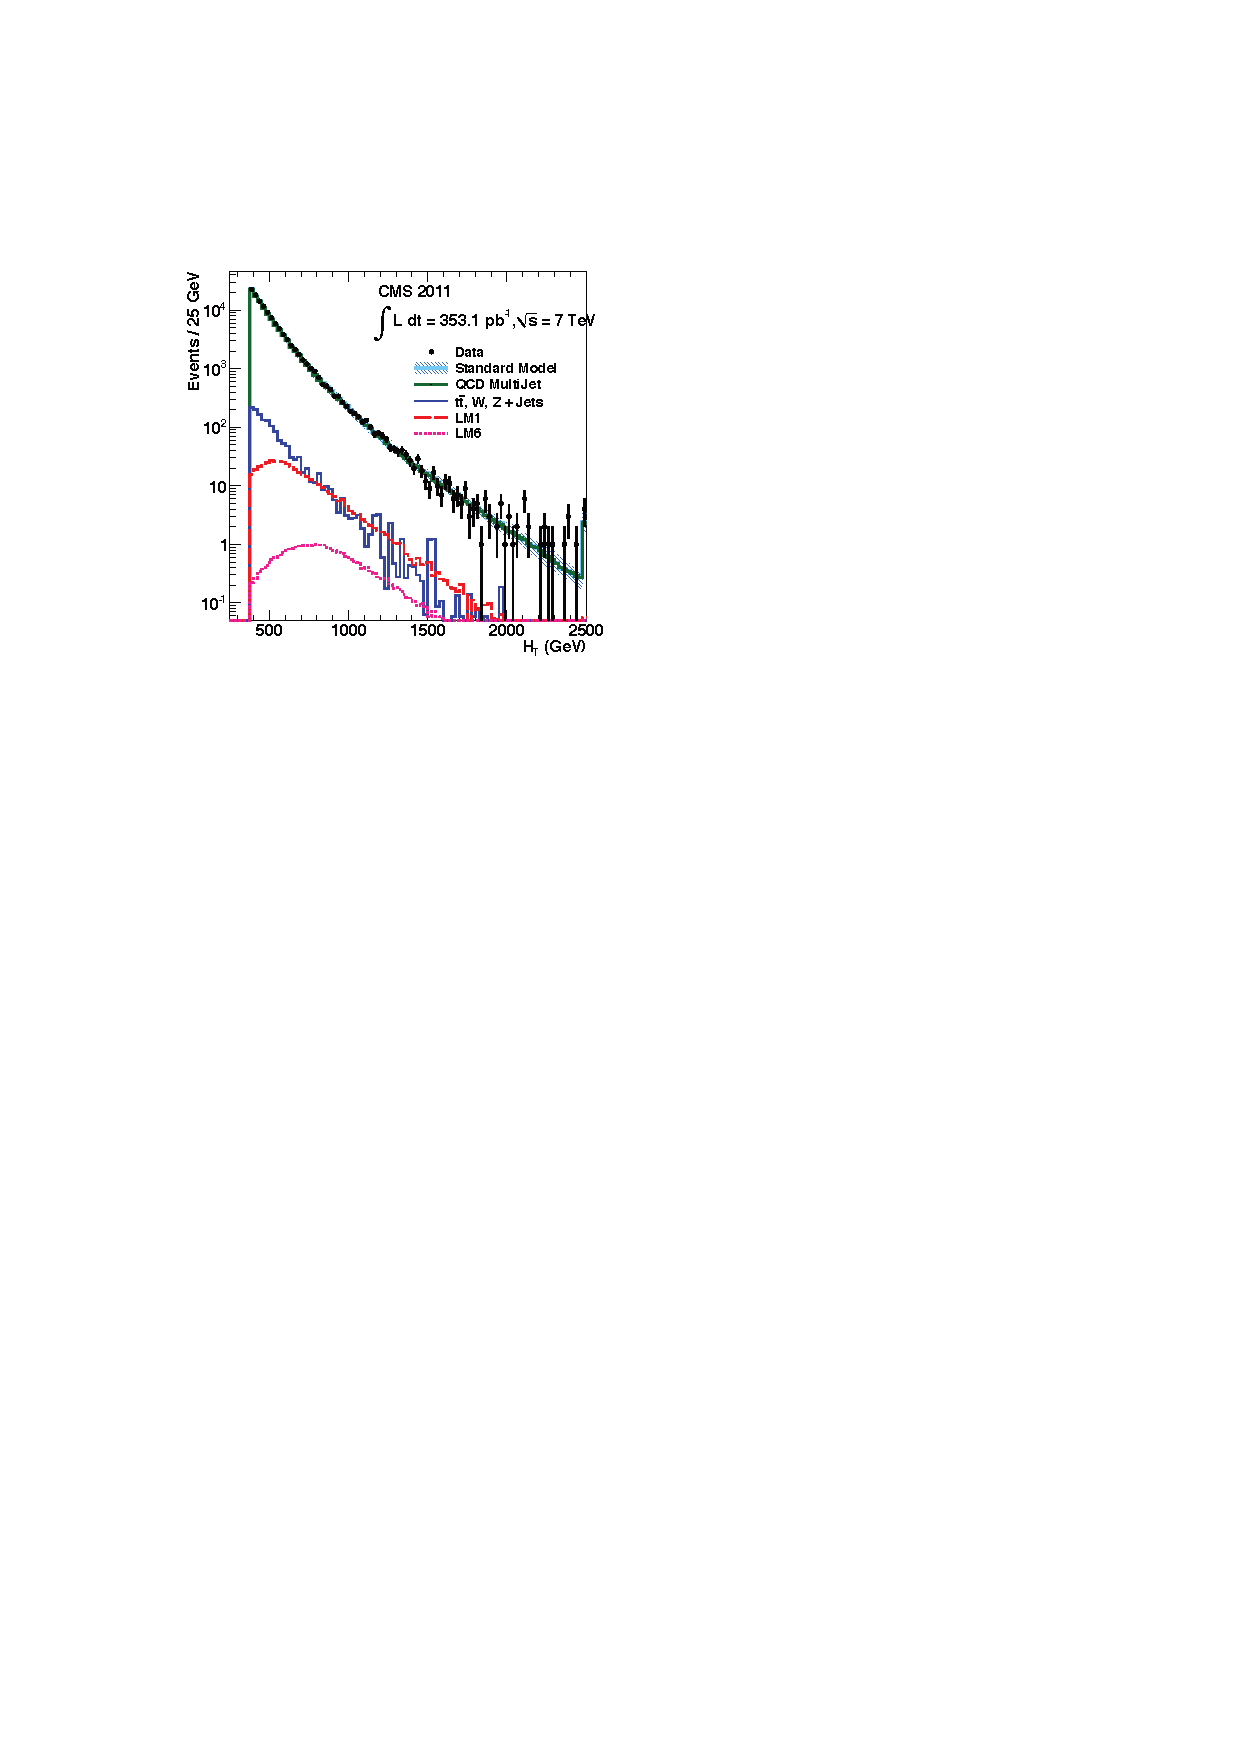
\includegraphics[width=0.60\textwidth]{plots/nocuts_htdistribution.pdf}
\caption[Reconstructed offline \theht for 11.7fb$^{-1}$ of data after a basic pre-selection.]{Reconstructed offline $\theht$ for 11.7fb$^{-1}$ of data after a basic pre-selection. Sample is collected from prescaled \theht triggers. Overlaid are expectations from MC simulation of \ac{EWK} processes as well as a reference signal model (labelled D2 from Table.\ref{tab:sms_model_table}).}  
\label{fig:htqcdbackground}
\end{figure}

Additional \ac{SM} background from \ac{EWK} processes with genuine $\met$ from escaping neutrinos comprise the irreducible background within this search and come mainly from:

\begin{itemize}
\item $Z \rightarrow \nu\bar{\nu} +$ jets,
\item $W \rightarrow l\nu$ + jets in which a lepton falls outside of detector acceptance, or the lepton decays hadronically $\tau \rightarrow$ had ,
\item $t\bar{t}$ with at least one leptonic W decay,
\item small background contributions from DY, single top and Diboson (WW,ZZ,WZ) processes.
\end{itemize}

The search is designed to have a strong separation between events with genuine and ``fake'' $\met$ which is achieved primarily though the dimensionless kinematic variable, $\alphat$ \cite{PhysRevLett.101.221803}\cite{CMS:2008vya}.

\subsection{The $\alphat$ variable}
\label{subsec:alphatvariable}

For a perfectly measured di-jet QCD event, conservation laws dictate that they must be produced back-to-back and of equal magnitude. However in di-jet events with real $\met$, both of these jets are produced independently of one another, depicted in Figure \ref{fig:susytopology}.
\begin{figure}[!h]
\centering
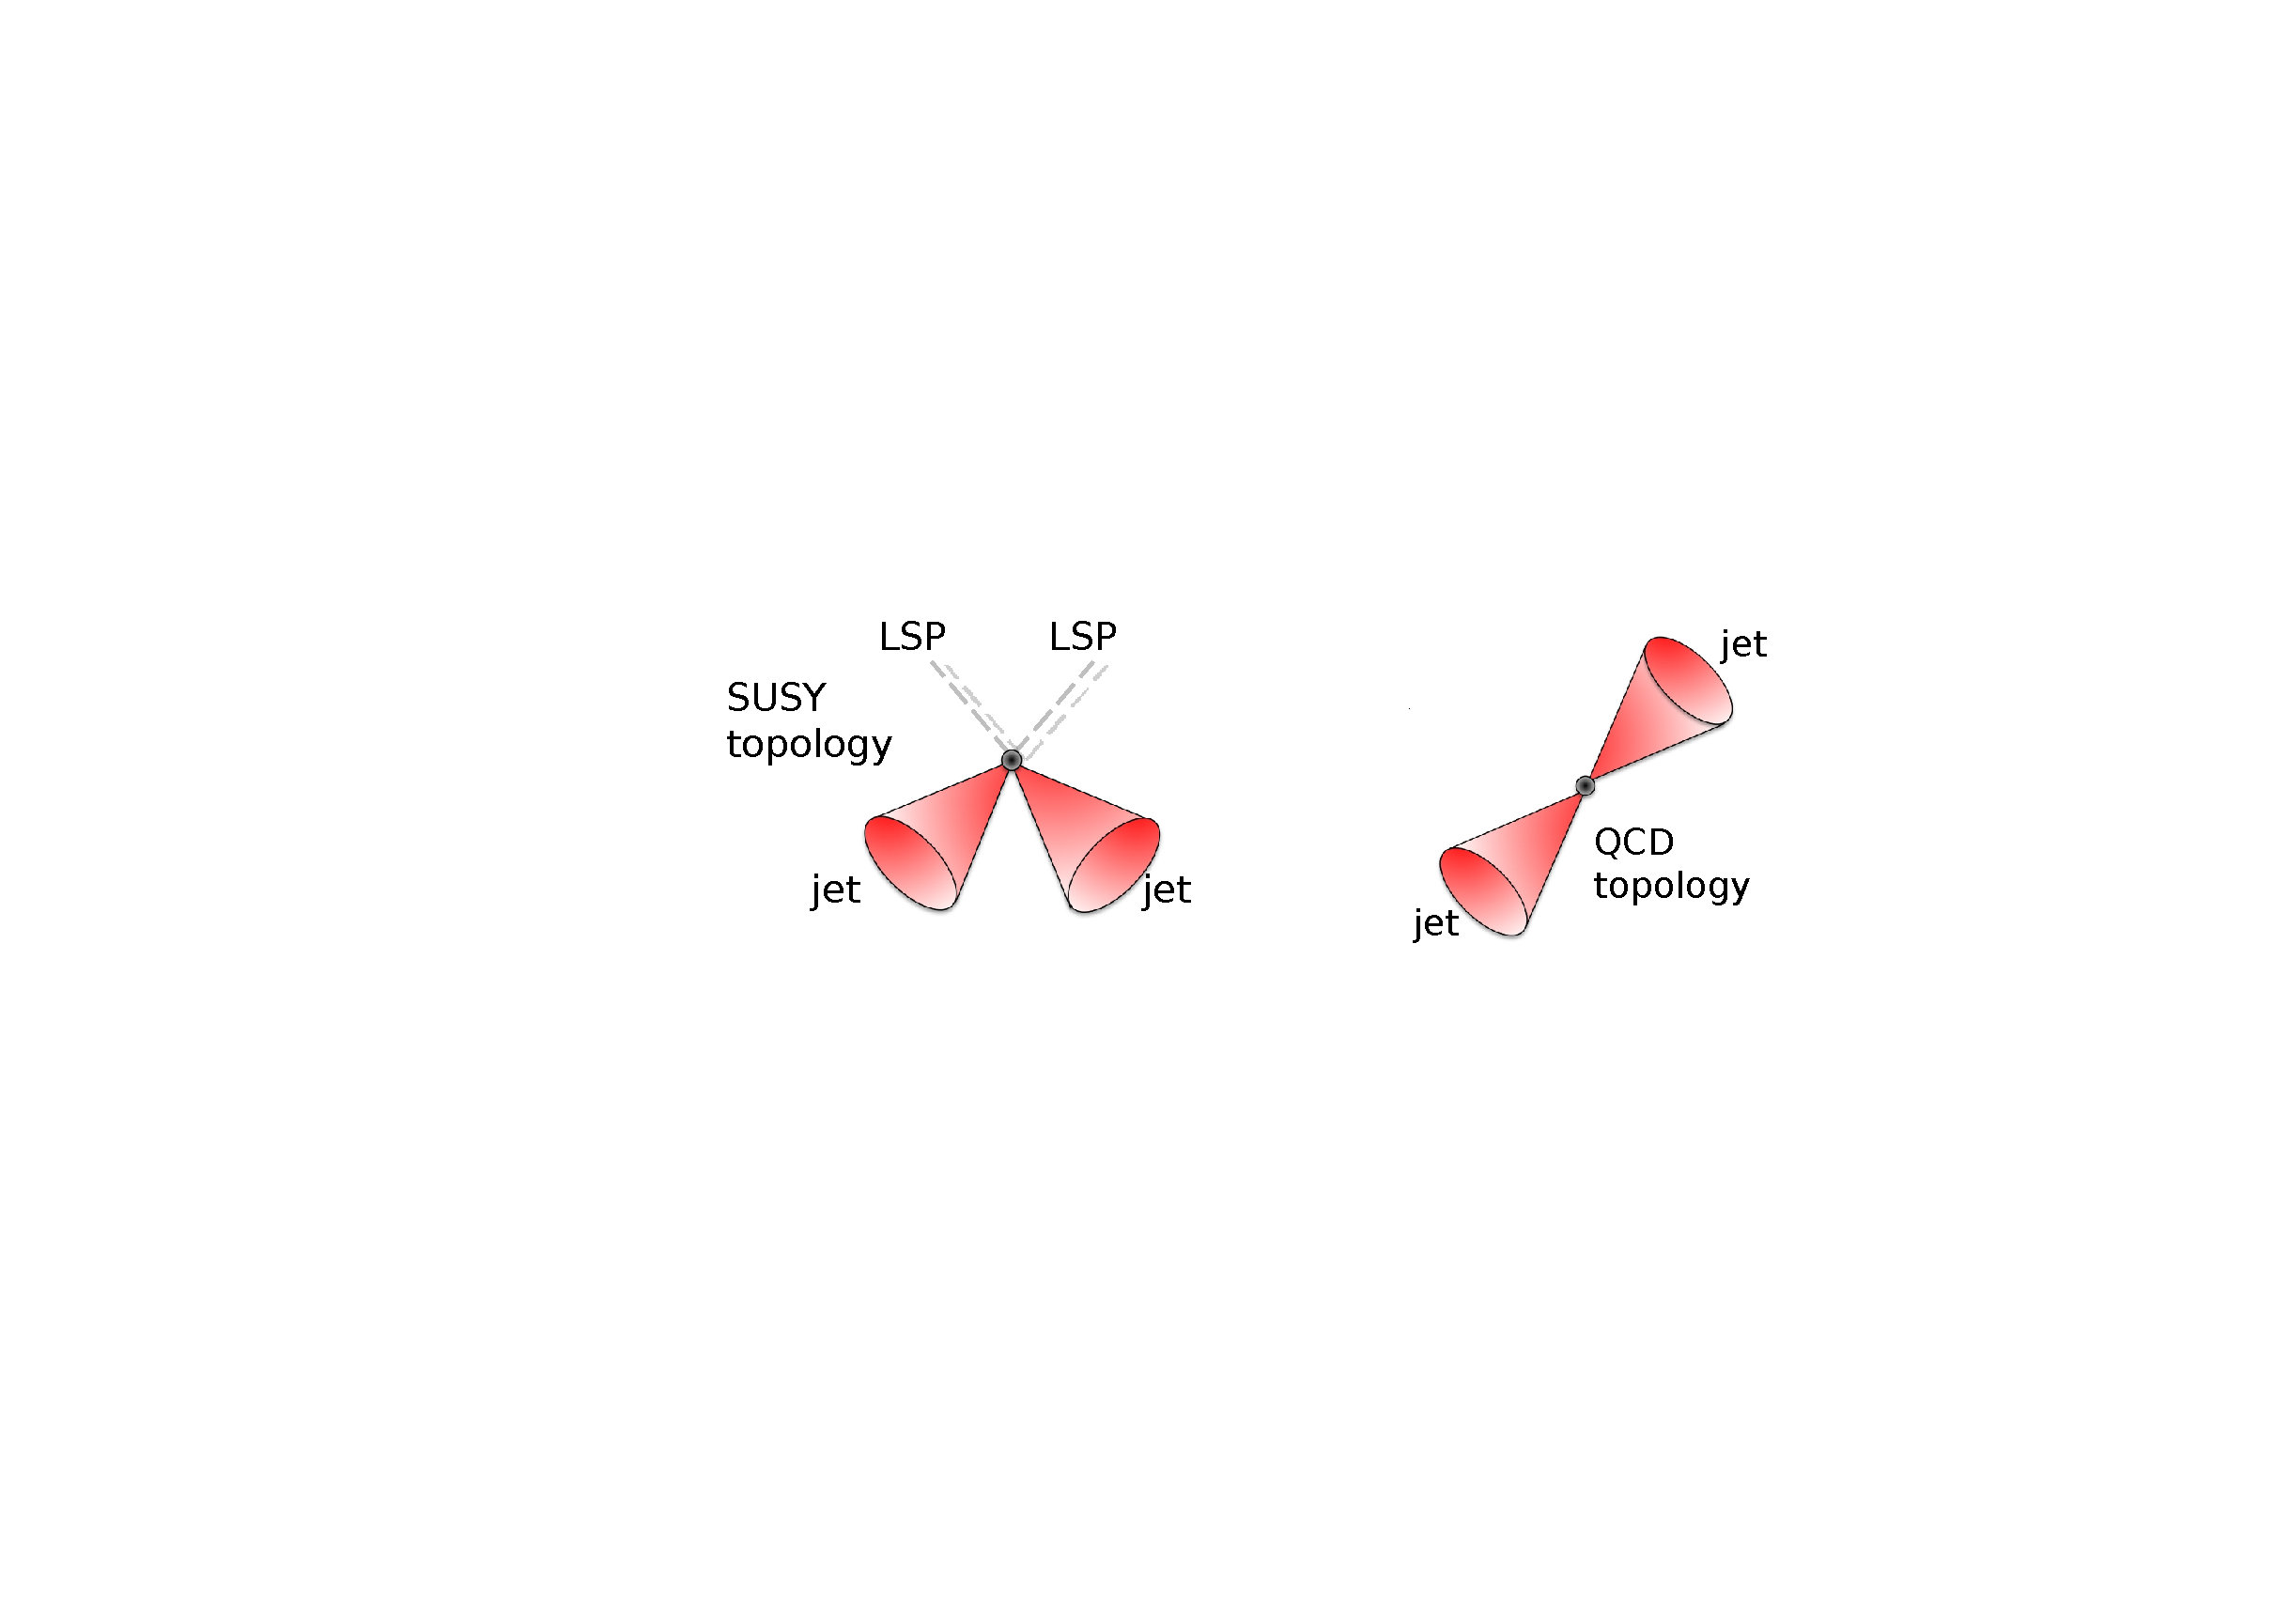
\includegraphics[width=0.90\textwidth]{plots/susy_topology.pdf}
\caption[The event topologies of background QCD diet events (right) and a generic \ac{SUSY} signature with genuine $\met$ (left).]{The event topologies of background QCD diet events (right) and a generic \ac{SUSY} signature with genuine $\met$ (left).}  
\label{fig:susytopology}
\end{figure}

 Exploiting this feature leads to the formulation of $\alphat$ in di-jet systems defined as,

\begin{equation}
\alphat = \frac {E^{j2}_{T}}{M_{T}},
\end{equation} 

where $E^{j2}_{T}$ is the transverse energy of the least energetic of the two jets and $M_{T}$ defined as:

\begin{equation}
\label{eq:transmass}
M_{T} = \sqrt{\left(\sum^{2}_{i=1}E^{j_{i}}_{T}\right)^{2}-\left(\sum^{2}_{i=1}p^{j_{i}}_{x}\right)^{2}-\left(\sum^{2}_{i=1}p^{j_{i}}_{y}\right)^{2}} \equiv \sqrt{H_{T}^{2} - \mht^{2}} .
\end{equation}

A perfectly balanced di-jet event i.e. $E_{T}^{j_{1}} = E_{T}^{j_{2}}$ would give an $\alphat = 0.5$, where as events with jets which are not back-to-back, for example in events in which
a W or Z recoils off a system of jets, $\alphat$ can achieve values in excess of 0.5.

$\alphat$ can be extended to apply to any arbitrary number of jets, undertaken by modelling a system of $n$ jets as a di-jet system, through the formation of two pseudo-jets \cite{CMS-PAS-SUS-09-001}. The two pseudo-jets are built by merging the jets present in the event such that the 2 pseudo-jets are chosen to be as balanced as possible, i.e the $\Delta$ \theht $\equiv \lvert E_{T}^{pj_{1}} - E_{T}^{pj_{2}}\rvert$ is minimised between the two pseudo jets. Using Equation (\ref{eq:transmass}), $\alphat$ can be rewritten as,

\begin{equation}
\label{eq:alphatmht}
\alphat = \frac{1}{2} \frac {\theht - \Delta\theht}{\sqrt{\theht^{2}-\mht^{2}}}= \frac{1}{2}\frac{1-\Delta\theht/\theht}{\sqrt{1-(\mht/\theht)^{2}}}.
\end{equation}

The distribution of $\alphat$ for the two jet categories used within this analysis, 2,3 and $\geq 4$ jets, is shown in the Figure.\ref{fig:fullalphatdistribution}, demonstrating the ability of the $\alphat$ variable to discriminate between multi jet events and \ac{EWK} processes with genuine $\met$ in the final state.  

\begin{figure}[ht]
\centering
\begin{minipage}[b]{0.48 \linewidth}
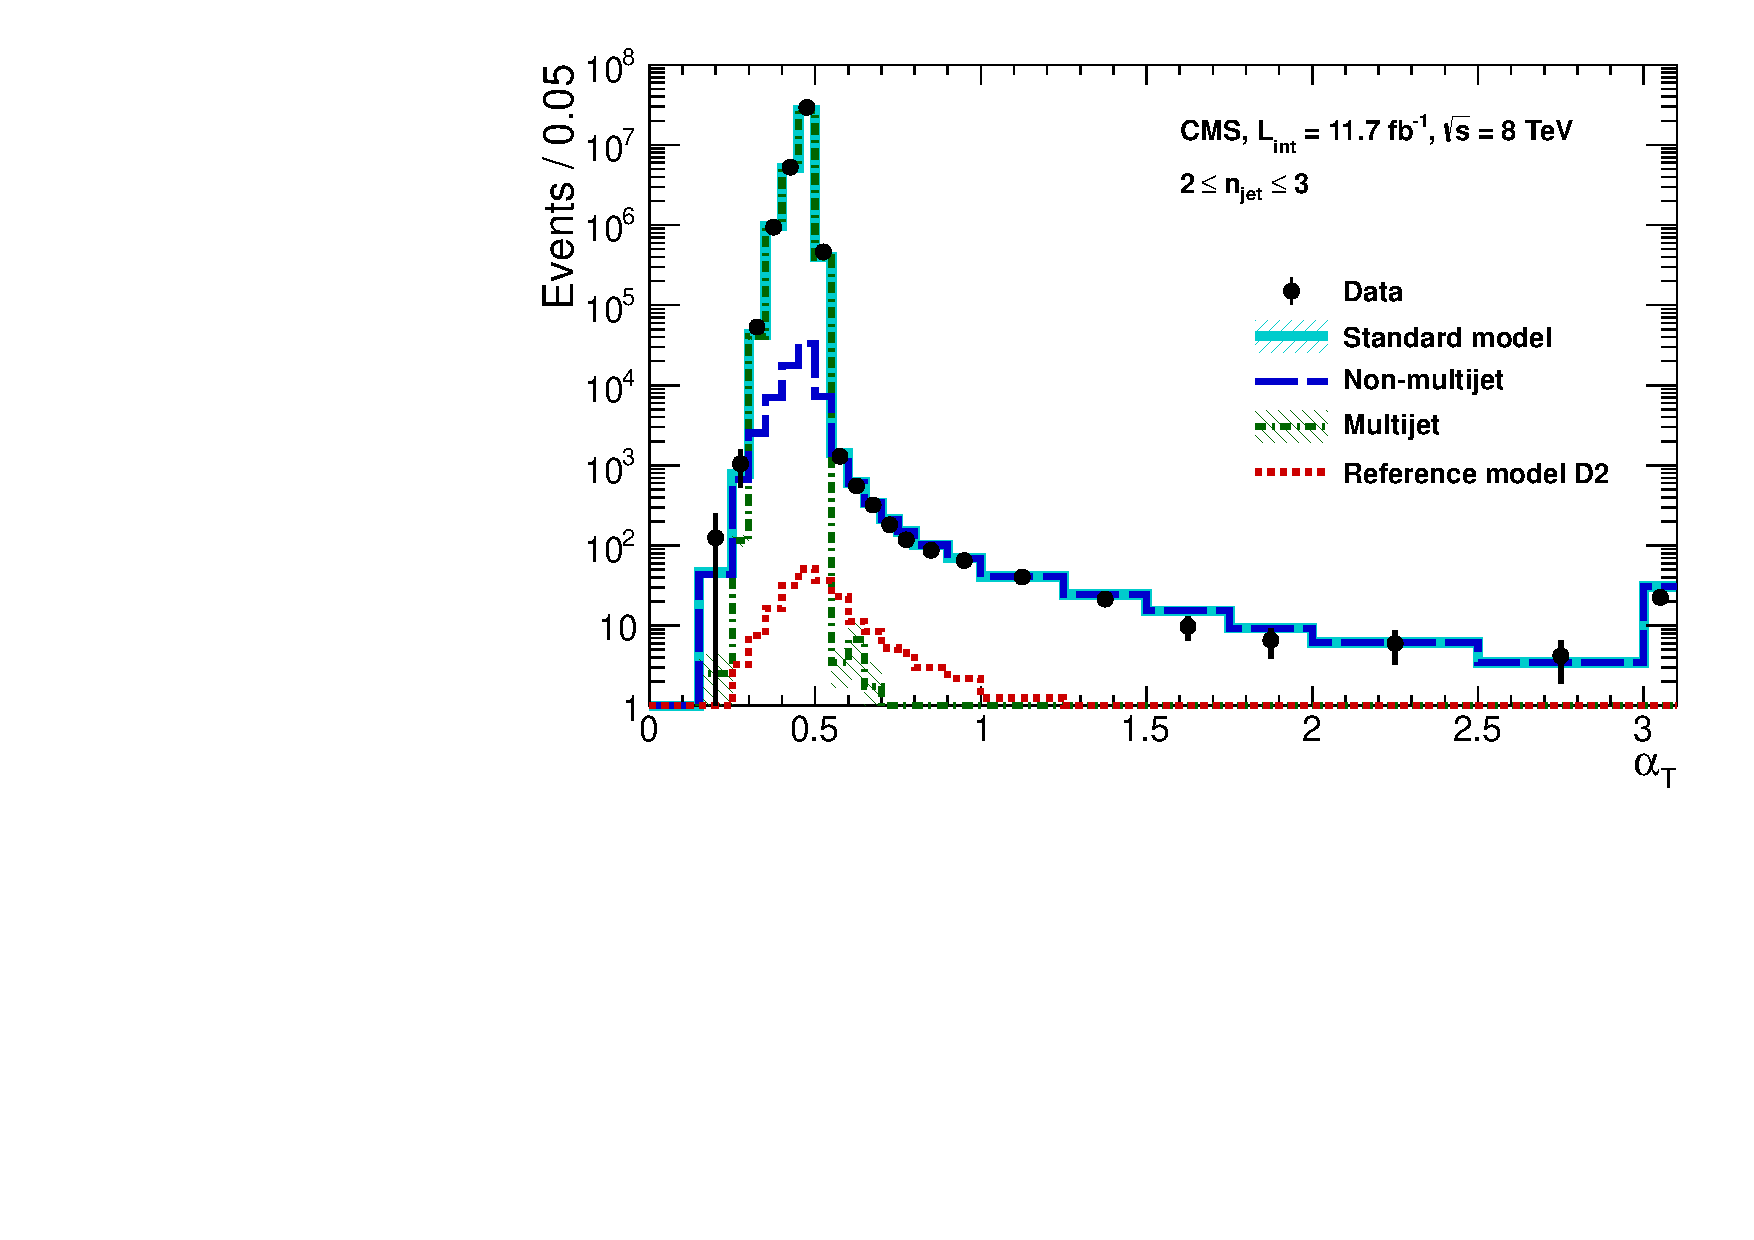
\includegraphics[width = 1.0\linewidth,height = 7.0cm]{plots/alphat_low.pdf}
\end{minipage}
\quad
\begin{minipage}[b]{0.48\linewidth}
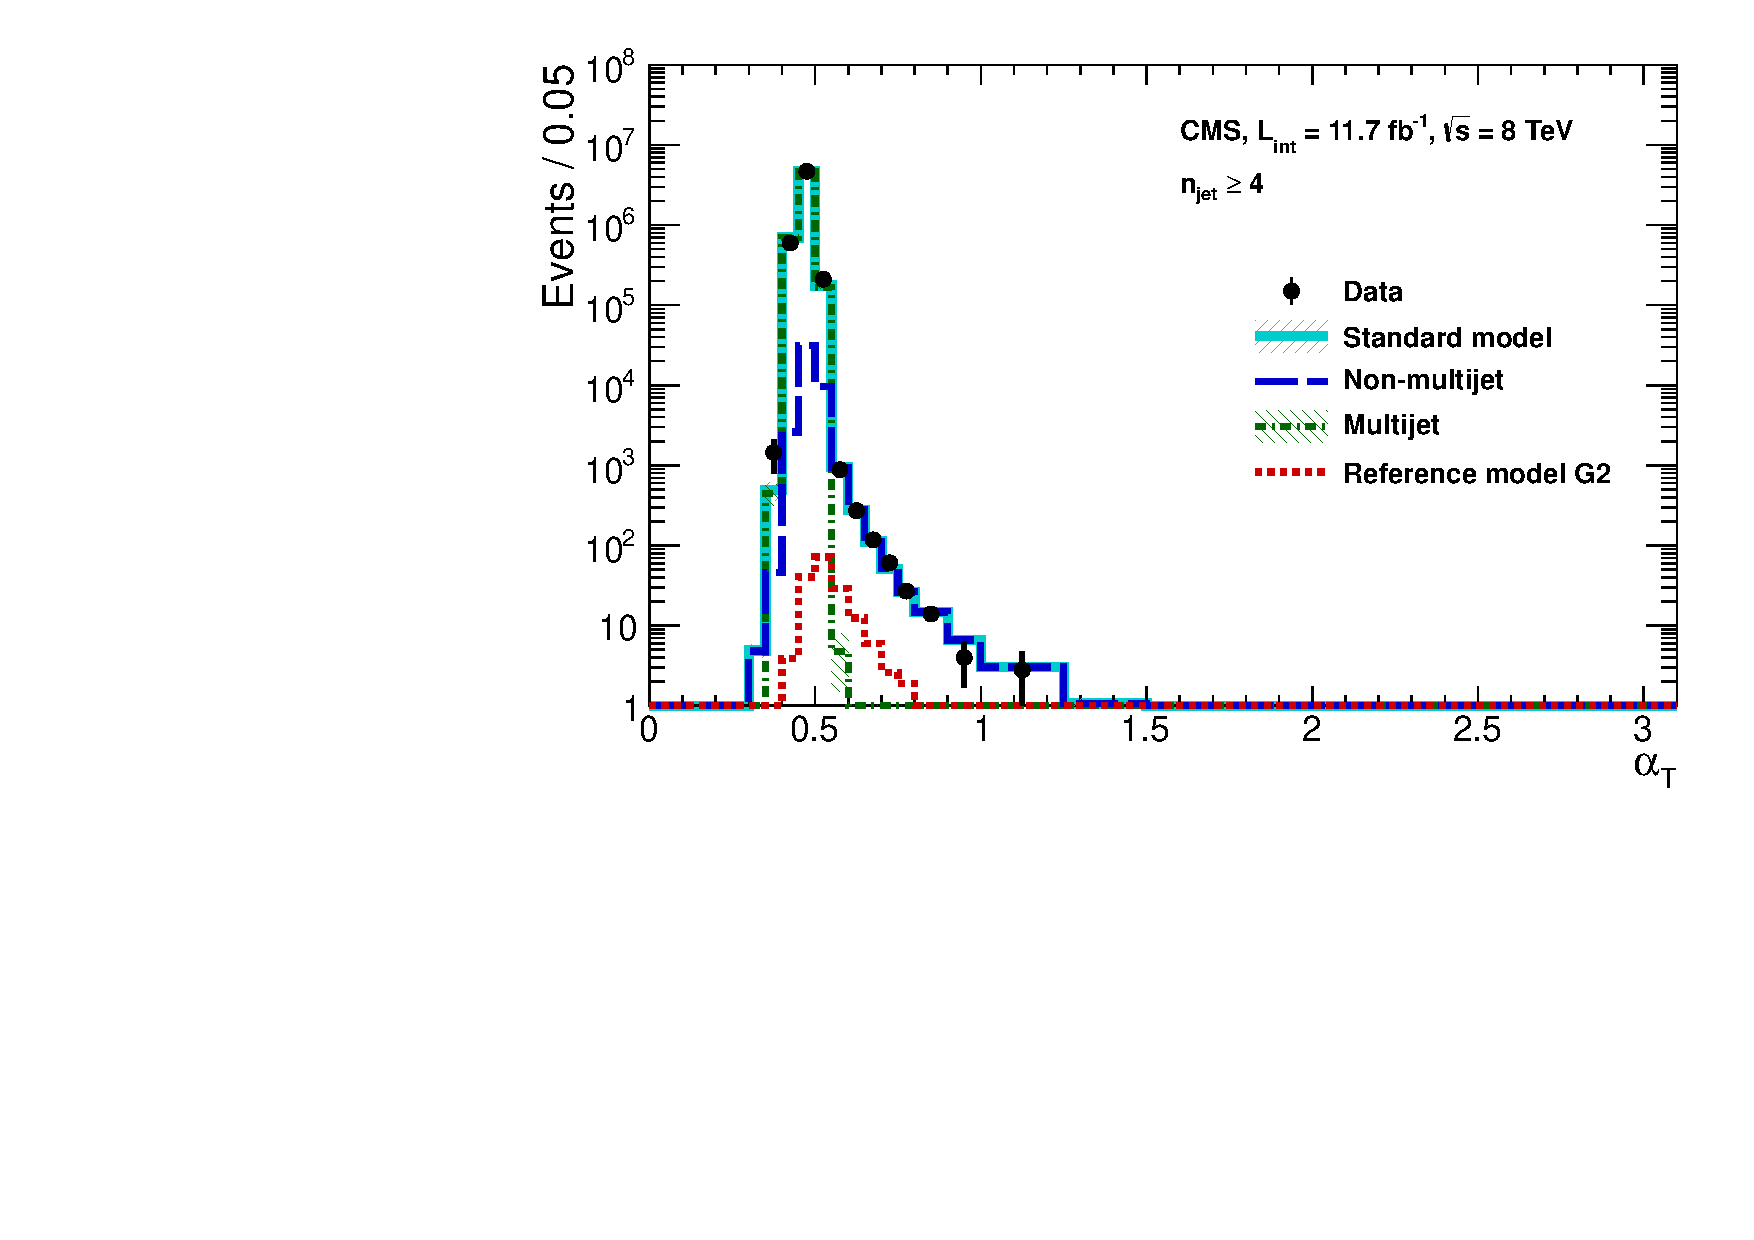
\includegraphics[width = 1.0\linewidth, height = 7.0cm]{plots/alphat_high.pdf}
\end{minipage}
\caption[ The $\alphat$ distributions for the low 2-3 (left) and high $\geq 4$ (right) jet multiplicities after a full analysis selection and shown for $\theht > 375$.]{The $\alphat$ distributions for the low 2-3 (left) and high $\geq 4$ (right) jet multiplicities after a full analysis selection and shown for $\theht > 375$ . Data is collected using both prescaled $\theht$ triggers and dedicated $\alphat$ triggers for below and above $\alphat = 0.55$ respectively. . Expected yields as given by simulation are also shown for multijet events (green dash-dotted line), \ac{EWK} backgrounds with genuine $\met$ (blue long-dashed line), the sum of all \ac{SM} processes (cyan solid line) and the reference signal model D2 (left, red dotted line) or G2 (right, red dotted line). }
\label{fig:fullalphatdistribution}
\end{figure}

The $\alphat$ requirement used within the search is chosen to be $\alphat >$ 0.55 to ensure that the QCD multijet background is negligible even in the presence of moderate jet mis-measurement. There still remains other effects which can cause multijet events to artificially have a large $\alphat$ value, which are discussed in detail in Section (\ref{subsec:eventselection}).  


\section{Search Strategy}
\label{subsec:searchstrategy}

The aim of the analysis presented in this thesis is to identify an excess of events in data over the \ac{SM} background expectation in multi-jet final states and significant $\met$. The essential suppression of the dominant QCD background for such a search is addressed by the $\alphat$ variable described in the previous section. For estimation of the remaining \ac{EWK} backgrounds, three independent data control samples are used to predict the different processes that compose the background :

\begin{itemize}
\item \mupjets to determine W + jets, \ttbar and single top backgrounds,
\item \gpjets  to determine the irreducible \zinv + jets background,
\item \dimupjets to determine the irreducible \zinv + jets background.
\end{itemize}

These control samples are chosen to both be rich in specific \ac{EWK} processes, be free of QCD multi-jet events and to also be kinematically similar to the hadronic signal region that they are estimating the backgrounds of, see Section (\ref{subsec:controlsampledefinition}).

To remain inclusive to a large range of possible \ac{SUSY} models, the signal region is binned in the following categories to allow for increased sensitivity in the interpretation of results for different \ac{SUSY} topologies:

\begin{itemize}

\item[] \textbf{Sensitivity to a range of \ac{SUSY} mass splittings}

The hadronic signal region is defined by \theht $>$ 275, divided into eight bins in \theht. 

\begin{itemize}
\item Two bins of width 50 \GeV in the range 275 $<$ \theht $<$ 375 \GeV,
\item five bins of width 100 \GeV in the range 375 $<$ \theht$<$ 875 \GeV,
\item and a final open bin, \theht $>$ 875 \GeV.
\end{itemize}

The choice at low \theht is driven primarily by trigger constraints. The mass difference between the \ac{LSP} and the particle that it decays from is an important factor in the amount of hadronic activity in the event. 

A large mass splitting will lead to hard high \pt jets which contribute to the \theht sum. From Figure \ref{fig:htqcdbackground} it can be seen that the \ac{SM} background falls sharply at high \theht values, therefore a large number of \theht bins will lead to easier of identification of such signals. Conversely smaller mass splittings lead to softer jet \pt's which will subsequently fall into the lower \theht range.

\item[] \textbf{Sensitivity to production method of \ac{SUSY} particles}

The production mechanism of any potential \ac{SUSY} signal can lead to different event topologies. One such way to discriminate between gluino ($g\widetilde{g}$ - ``high multiplicity''), and direct squark ($q\widetilde{q}$ - ``low multiplicity'') induced production of \ac{SUSY} particles is realised through the number of reconstructed jets in the final state.  

The analysis is thus split into two jet categories : 2-3 jets , $\geq$ 4 jets to give sensitivity to both of these mechanisms. 

\item[] \textbf{Sensitivity to  ``Natural \ac{SUSY}'' via tagging jets from b-quarks}

Jets originating from bottom quarks (b-jets) are identified through vertices that are displaced with respect to the primary interaction. The algorithm used to tag b-jets is the \acf{CSVM} tagger, described within Section (\ref{subsec:cmsobjects-btagging}). A cut is placed on the discriminator variable of $> 0.679$, leading to a gluon/light-quark mis-tag rate of 1\% and a jet p$_{\text{T}}$ dependant b-tagging efficiency of 60-70\% \cite{btag8tev}.

Natural \ac{SUSY} models would be characterised through final-state signatures rich in bottom quarks. A search relying on methods to identify jets originating from bottom quarks through b-tagging, will significantly improve the sensitivity to this class of signature. 

This is achieved via the binning of events in the signal region according to the number of b-tagged jets reconstructed in each event, in the following: 0,1,2,3,$\geq$ 4 b-tag categories . In the highest $\geq$ 4 b-tag category due to a limited number of expected signal and background, just three \theht bins are employed: 275-325 \GeV, 325-375 \GeV, $\geq$ 375 \GeV.

This characterisation is identically mirrored in all control samples, with the information from all samples and b-tag categories used simultaneously in the likelihood model (see Chapter \ref{chap:SUSYresults}) in order to interpret the results in a coherent and powerful way.

\end{itemize}
 
 The combination of the \theht, jet multiplicity and b-tag categorisation of the signal region as described above, resultantly leads to 67 different bins in which the analysis is interpreted in, which is depicted in Figure \ref{fig:analysisbinning}. 
 
 \begin{figure}[!h]
 \centering
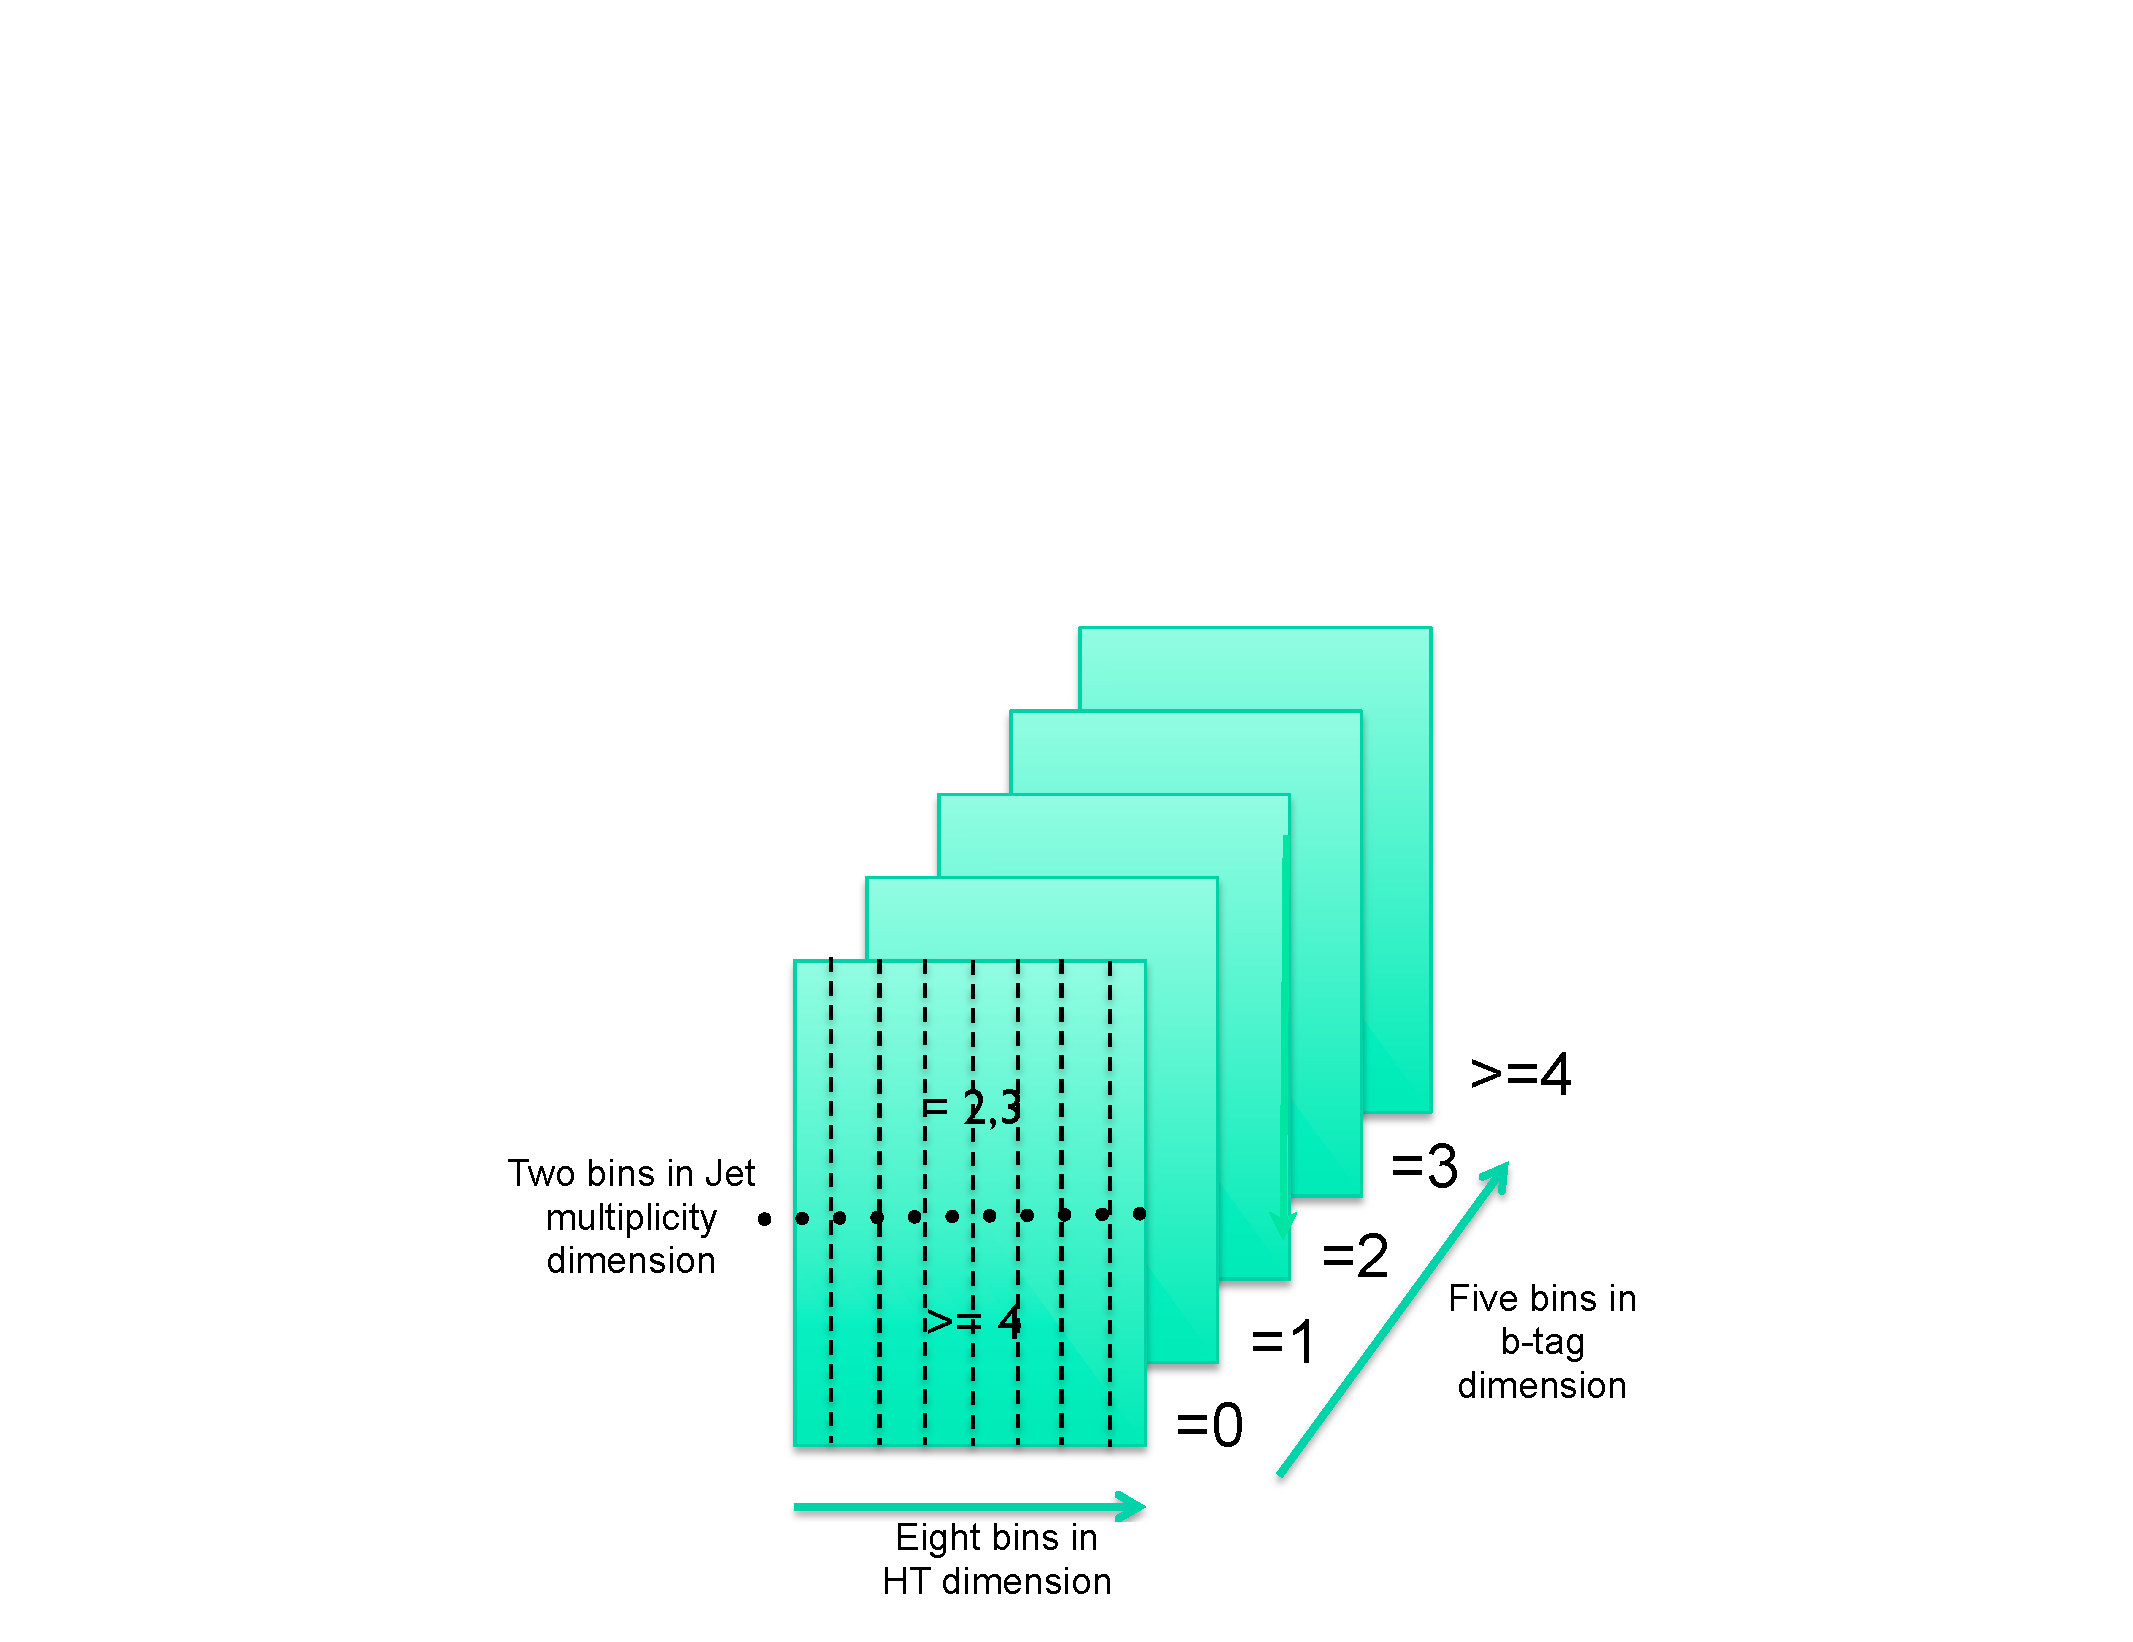
\includegraphics[width=0.70\textwidth]{plots/analysis_binning.pdf}
\caption[Pictorial depiction of the analysis strategy employed by the $\alphat$ search to increase sensitivity to a wide spectra of \ac{SUSY} models.]{Pictorial depiction of the analysis strategy employed by the $\alphat$ search to increase sensitivity to a wide spectra of \ac{SUSY} models.}  
\label{fig:analysisbinning}
\end{figure}



\subsection{Physics Objects}
\label{subsec:physicsobjects}

The physics objects used in the analysis defined below, follow the recommendation of the various \ac{CMS} \acf{POGs}. 

\begin{itemize}

\item \textbf{Jets}

The jets used in this analysis are CaloJets, reconstructed as described in Section (\ref{subsec:cmsobjects-jets}) using the anti-k$_{T}$ jet clustering algorithm. 

To ensure the jet object falls within the calorimeter systems a pseudo-rapidity requirement of \abeta $<$ 3 is applied. Each jet must pass a ``loose'' identification criteria to reject jets resulting from unphysical energy, the criteria of which are detailed in Table \ref{tabapp:calojetid} of Appendix (\ref{app:noise})  \cite{CMS-PAS-JME-09-008}.

\item \textbf{Muons}

Muons are selected in the \mupjets and \dimupjets control samples, and vetoed in the signal region. The same cut based identification criteria is applied to muons in both search regions and is summarised in Table \ref{tab:muonidtable} \cite{1748-0221-7-10-P10002}.

\begin{table}[h!]
\begin{center}
\begin{tabular*}{0.5\textwidth}{@{\extracolsep{\fill}}ll}
\cline{1-2}
Categories & Criteria \\ 
\cline{1-2}
Global Muon & True \\
PFMuon & True \\
$\chi^{2}$ & $<$ 10 \\
Muon chamber hits & $>$ 0 \\
Muon station hits & $>$ 1 \\
Transvere impact d$_{xy}$ & $<$ 0.2mm \\
Longitudinal distance d$_{z}$ & $<$ 0.5mm \\
Pixel hits & $>$ 0\\
Track layer hits & $>$ 5 \\
PF Isolation (DeltaB corrected) & $<$0.12 \\
\cline{1-2}
\end{tabular*}
\end{center}
\caption[Muon Identification criteria used within the analysis for selection/veto purposes in the muon control/signal selections.]{Muon Identification criteria used within the analysis for selection/veto purposes in the muon control/signal selections.}
\label{tab:muonidtable}
\end{table}

Additionally muons are required to be within the acceptance of the muon tracking systems. For the muon control samples, trigger requirements necessitate a \abeta $<$ 2.1 for the selection of muons. In the signal region where muons are vetoed these conditions are relaxed to  \abeta $<$ 2.5 and a minimum threshold of \pt $> 10 $ \GeV is required of muon objects. 

\item \textbf{Photons} 

Photons are selected within the \gpjets control sample and vetoed in all other selections. Photons are identified in both cases according to the cut based criteria listed in Table \ref{tab:photonidtable} \cite{CMS-PAS-SUS-12-018}.

\begin{table}[h!]
\begin{center}
\begin{tabulary}{0.80\textwidth}{LL}
\cline{1-2}
Variable & Definition \\ 
\cline{1-2}
H/E $< $ 0.05  \qquad\qquad\qquad\qquad\qquad\qquad & The ratio of hadronic energy in the \ac{HCAL} tower directly behind the \ac{ECAL} super-cluster and the \ac{ECAL} super-cluster itself. \\
$\sigma_{i\eta i\eta}< 0.011$ \qquad\qquad\qquad\qquad\qquad\qquad\qquad\qquad  & The log energy weighted width ($\sigma$), of the extent of the shower in the $\eta$ dimension.\\
R9 $<$ 1.0 & The ratio of the energy of the 3$\times$3 crystal core of the super-cluster compared to the total energy stored in the 5$\times$5 super-cluster. \\
Combined Isolation $<$ 6 \GeV &  The photons are required to be isolated with no electromagnetic or hadronic activity within a radius $\Delta$R = 0.3 of the photon object. A combination of the pileup subtracted \cite{Cacciari:2007fd}, \ac{ECAL}, \ac{HCAL} and tracking isolation sums are used to determine the combined total isolation value.  \\
\cline{1-2}
\end{tabulary}
\end{center}
\caption[Photon Identification criteria used within the analysis for selection/veto purposes in the \gpjets control/signal selections. ]{Photon Identification criteria used within the analysis for selection/veto purposes in the \gpjets control/signal selections.}
\label{tab:photonidtable}
\end{table}

Photon objects are also required to have a minimum momentum of \pt $>$ 25 \GeV.

\item \textbf{Electrons}

Electron identification is defined for veto purposes. They are selected according to the following cut-based criteria listed in Table \ref{tab:electronidtable}, utilising PF-based isolation.

\begin{table}[h!]
\begin{center}
\begin{tabular*}{0.5\textwidth}{@{\extracolsep{\fill}}lcc}
\cline{1-3}
Categories & Barrel &  EndCap\\ 
\cline{1-3}
$\Delta \eta_{In}$ & 0.007 & 0.009 \\
$\Delta \phi_{In}$ & 0.15 & 0.10 \\
$\sigma_{i\eta i\eta}$ & 0.01 & 0.03 \\
H/E & 0.12 & 0.10 \\
d0 (vtx) & 0.02 & 0.02 \\
dZ (vtx) & 0.20 & 0.20 \\
$\lvert$(1/E$_{ECAL}$ - 1/p$_{track}$)$\rvert$ & 0.05 & 0.05 \\
PF Combined isolation/\pt & 0.15 & 0.15 \\
Vertex fit probability & 10$^{-6}$ & 10$^{-6}$ \\
\cline{1-3}
\end{tabular*}
\end{center}
\caption[Electron Identification criteria used within the analysis for veto purposes.]{Electron Identification criteria used within the analysis for veto purposes.}
\label{tab:electronidtable}
\end{table}

Electrons are required to be identified at \abeta $<$ 2.5, with a minimum \pt $>$ 10 \GeV threshold to ensure that the electron falls within the tracking system of the detector.

\item \textbf{Noise and \met Filters}

A series of Noise filters are applied to veto events which contain spurious non-physical jets that are not picked up by the jet id, and events which give large unphysical \met values. These filters are listed within Table \ref{apptab:noiseid} of Appendix (\ref{app:noise}).

\end{itemize}


\subsection{Event Selection}
\label{subsec:eventselection}

The selection criteria for events within the analysis are detailed below. A set of common cuts are applied to both signal  (maximise acceptance to a range of \ac{SUSY} signatures),  and control samples (retain similar jet kinematics for background predictions), with additional selection cuts applied to each control sample to enrich the sample in a particular \ac{EWK} processes, see Section (\ref{subsec:controlsampledefinition}).

The jets considered in the analysis are required to have a transverse momentum \pt $>$ 50 \GeV, with a minimum of two jets required in the event. The highest \et jet is required to lie within the central tracker acceptance \abeta $<$ 2.5, and the two leading \pt jets must each have \pt $>$ 100\GeV.  Any event which has a jet with \pt $>$ 50 \GeV that either fails the ``loose'' identification criteria described in Section(\ref{subsec:physicsobjects}) or has \abeta $>$ 3.0, is rejected. Similarly events in which an electron,muon or photon fails object identification but pass \eta and \pt restrictions are identified as an ``odd'' lepton/photon and the event is vetoed.

At low \theht, the jet threshold requirements applied to be considered as part of the analysis and enter the \theht sum are scaled downwards. These are scaled down in order to not restrict phase space, preserving jet multiplicities and background admixture in the lower \theht bins, as listed in Table \ref{tab:jetthresholdtable}.

\begin{table}[h!]
\begin{center}
\begin{tabular*}{0.6\textwidth}{@{\extracolsep{\fill}}|l|c|c|}
\cline{1-3}
\theht bin & minimum jet \pt &  second leading jet \pt \\ 
\cline{1-3}
275 $<$ \theht$<$ 325 & 36.7 & 73.3 \\
325 $<$ \theht$<$ 375 & 43.3 & 86.6 \\
375 $<$ \theht & 50.0 & 100.0 \\

\cline{1-3}
\end{tabular*}
\end{center}
\caption[Jet thresholds used in the three \theht regions of the analysis.]{Jet thresholds used in the three \theht regions of the analysis.}
\label{tab:jetthresholdtable}
\end{table}

Within the signal region to suppress \ac{SM} processes with genuine \met from neutrinos, events containing isolated electrons or muons are vetoed. Furthermore to ensure a pure multi-jet topology, events are vetoed if an isolated photon is found with \pt $>$ 25 \GeV. 

An \alphat requirement of $>$ 0.55 is required to reduce the QCD multi-jet background to a negligible amount. Finally additional cleaning cuts are applied to protect against pathological deficiencies such as reconstruction failures or severe energy mis-measurements due to detector inefficiencies:

\begin{itemize}
\item Significant \mht can arise in events with no real \met due to multiple jets falling below the \pt threshold used for selecting jets. This in turn leads to events which can then incorrectly pass the \alphat requirements of the analysis. This effect can be negated by requiring that the missing transverse momentum reconstructed from jets alone does not greatly exceed the missing transverse momentum reconstructed from all of the detector's calorimeter towers,
\begin{equation}
R_{miss} = \mht / \met < 1.25. \nonumber
\end{equation}  

\item Fake \met and \mht can arise due to significant jet mis-measurements cause by a small number of non-functioning \ac{ECAL} regions. These regions absorb electromagnetic showers which are subsequently not added to the jet energy sum. To circumvent this problem the following procedure is employed : For each jet in the event, the angular separation

\begin{equation}
\Delta\phi_{j}^{*}\equiv \Delta\phi(p_{j}^{\rightarrow}-\sum_{i\neq j}p_{i}^{\rightarrow}),
\end{equation}

is calculated where that jet is itself removed from the event. Here $\Delta\phi^{*}$ is a measure of how aligned the \mht of an event is with a jet, a small value is compatible with the hypothesis of an inherently balanced event in
which a jet has been mis-measured. For every jet in a event with $\Delta\phi^{*} <$ 0.5, if the $\Delta R$ distance between the selected jet and the closest dead \ac{ECAL} region is also $<$ 0.3, then the event is rejected. Similarly events are rejected if the jet points within $\Delta R <$ 0.3 of the \ac{ECAL} barrel-endcap gap at \abeta $=$ 1.5.

\end{itemize}

Some of the key distributions of the data used in this analysis compared to MC simulation are shown in Figure \ref{fig:hadmcplots}. The MC samples are normalised to a luminosity of 11.7 \fb,  with no requirement placed upon the number of b-tagged jets or number of jets in the events. 

The distributions shown are presented for purely illustrative purposes, with the MC simulation itself not used in absolute term to estimate the yields from background processes, see Sections (\ref{subsec:controlsampledefinition},\ref{subsec:backgroundestimation}). However it is nevertheless important to demonstrate that good agreement exists between simulation and observation in data.

\begin{minipage}{\linewidth}
\centering
\begin{minipage}{.48\textwidth}
\centering
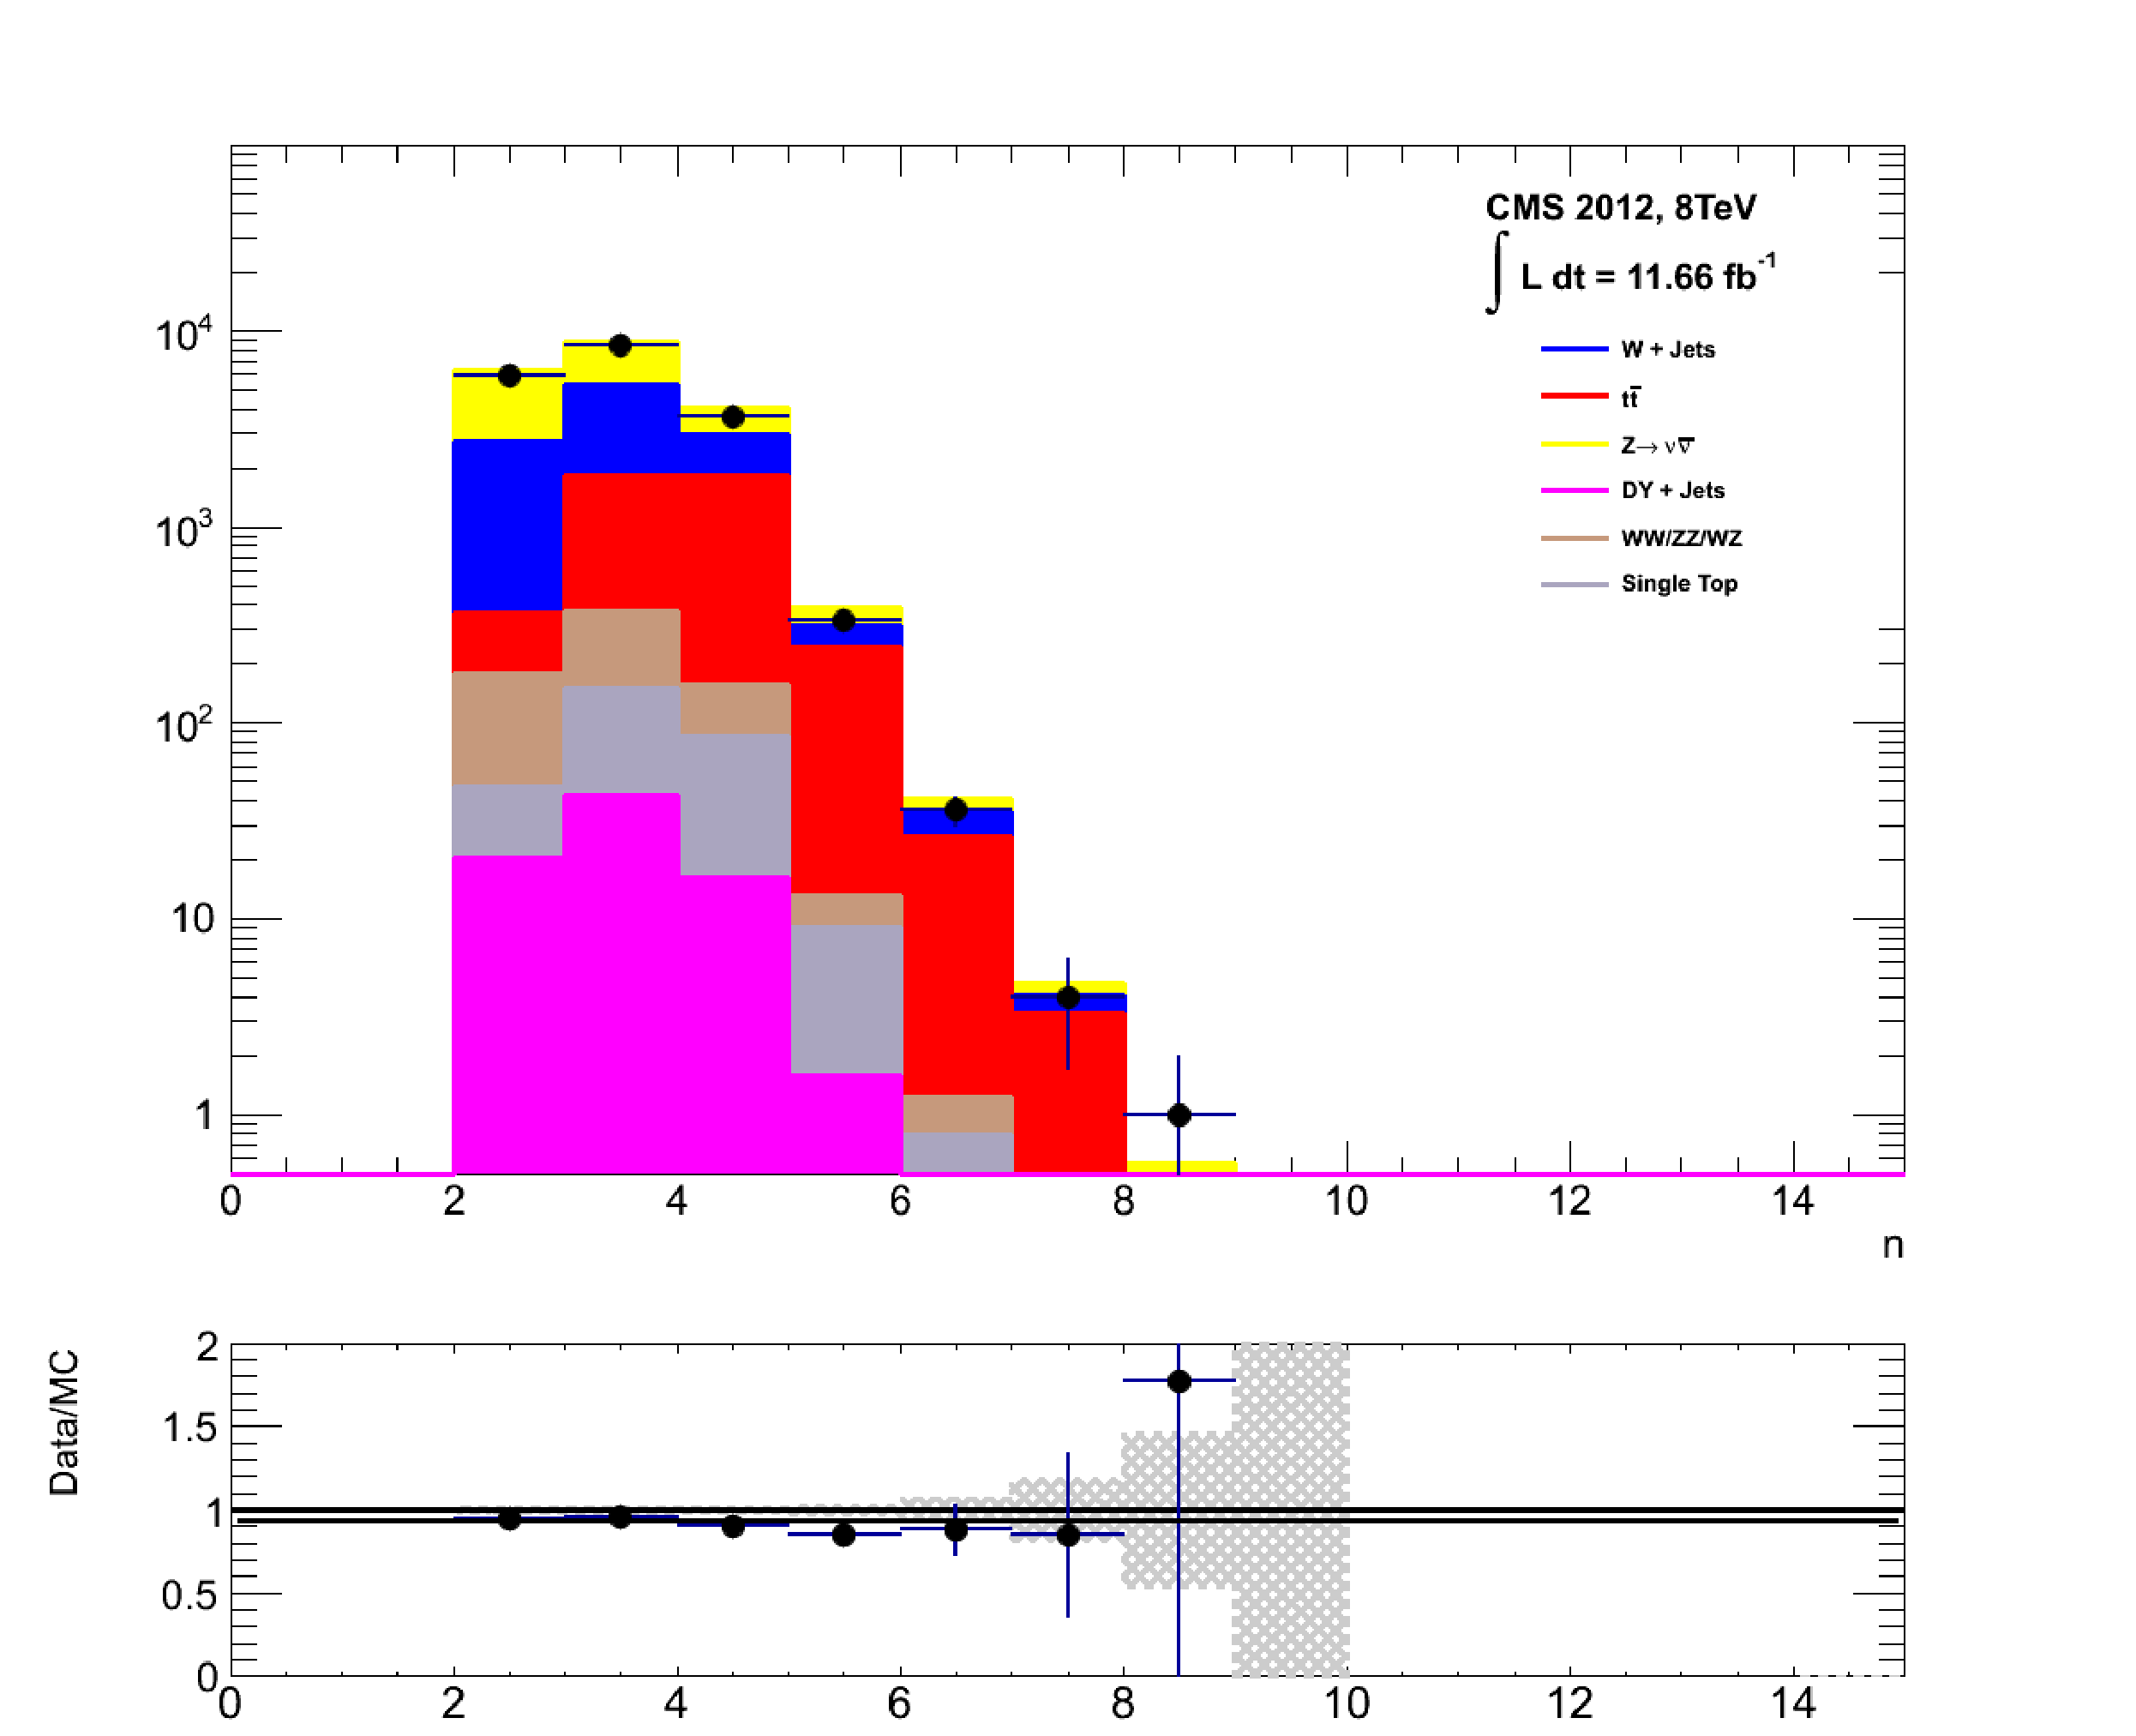
\includegraphics[width = 3.3in]{plots/had_njet_datamc.pdf}
(a) Jet Multiplicity
\end{minipage}
\begin{minipage}{.48\textwidth}
\centering
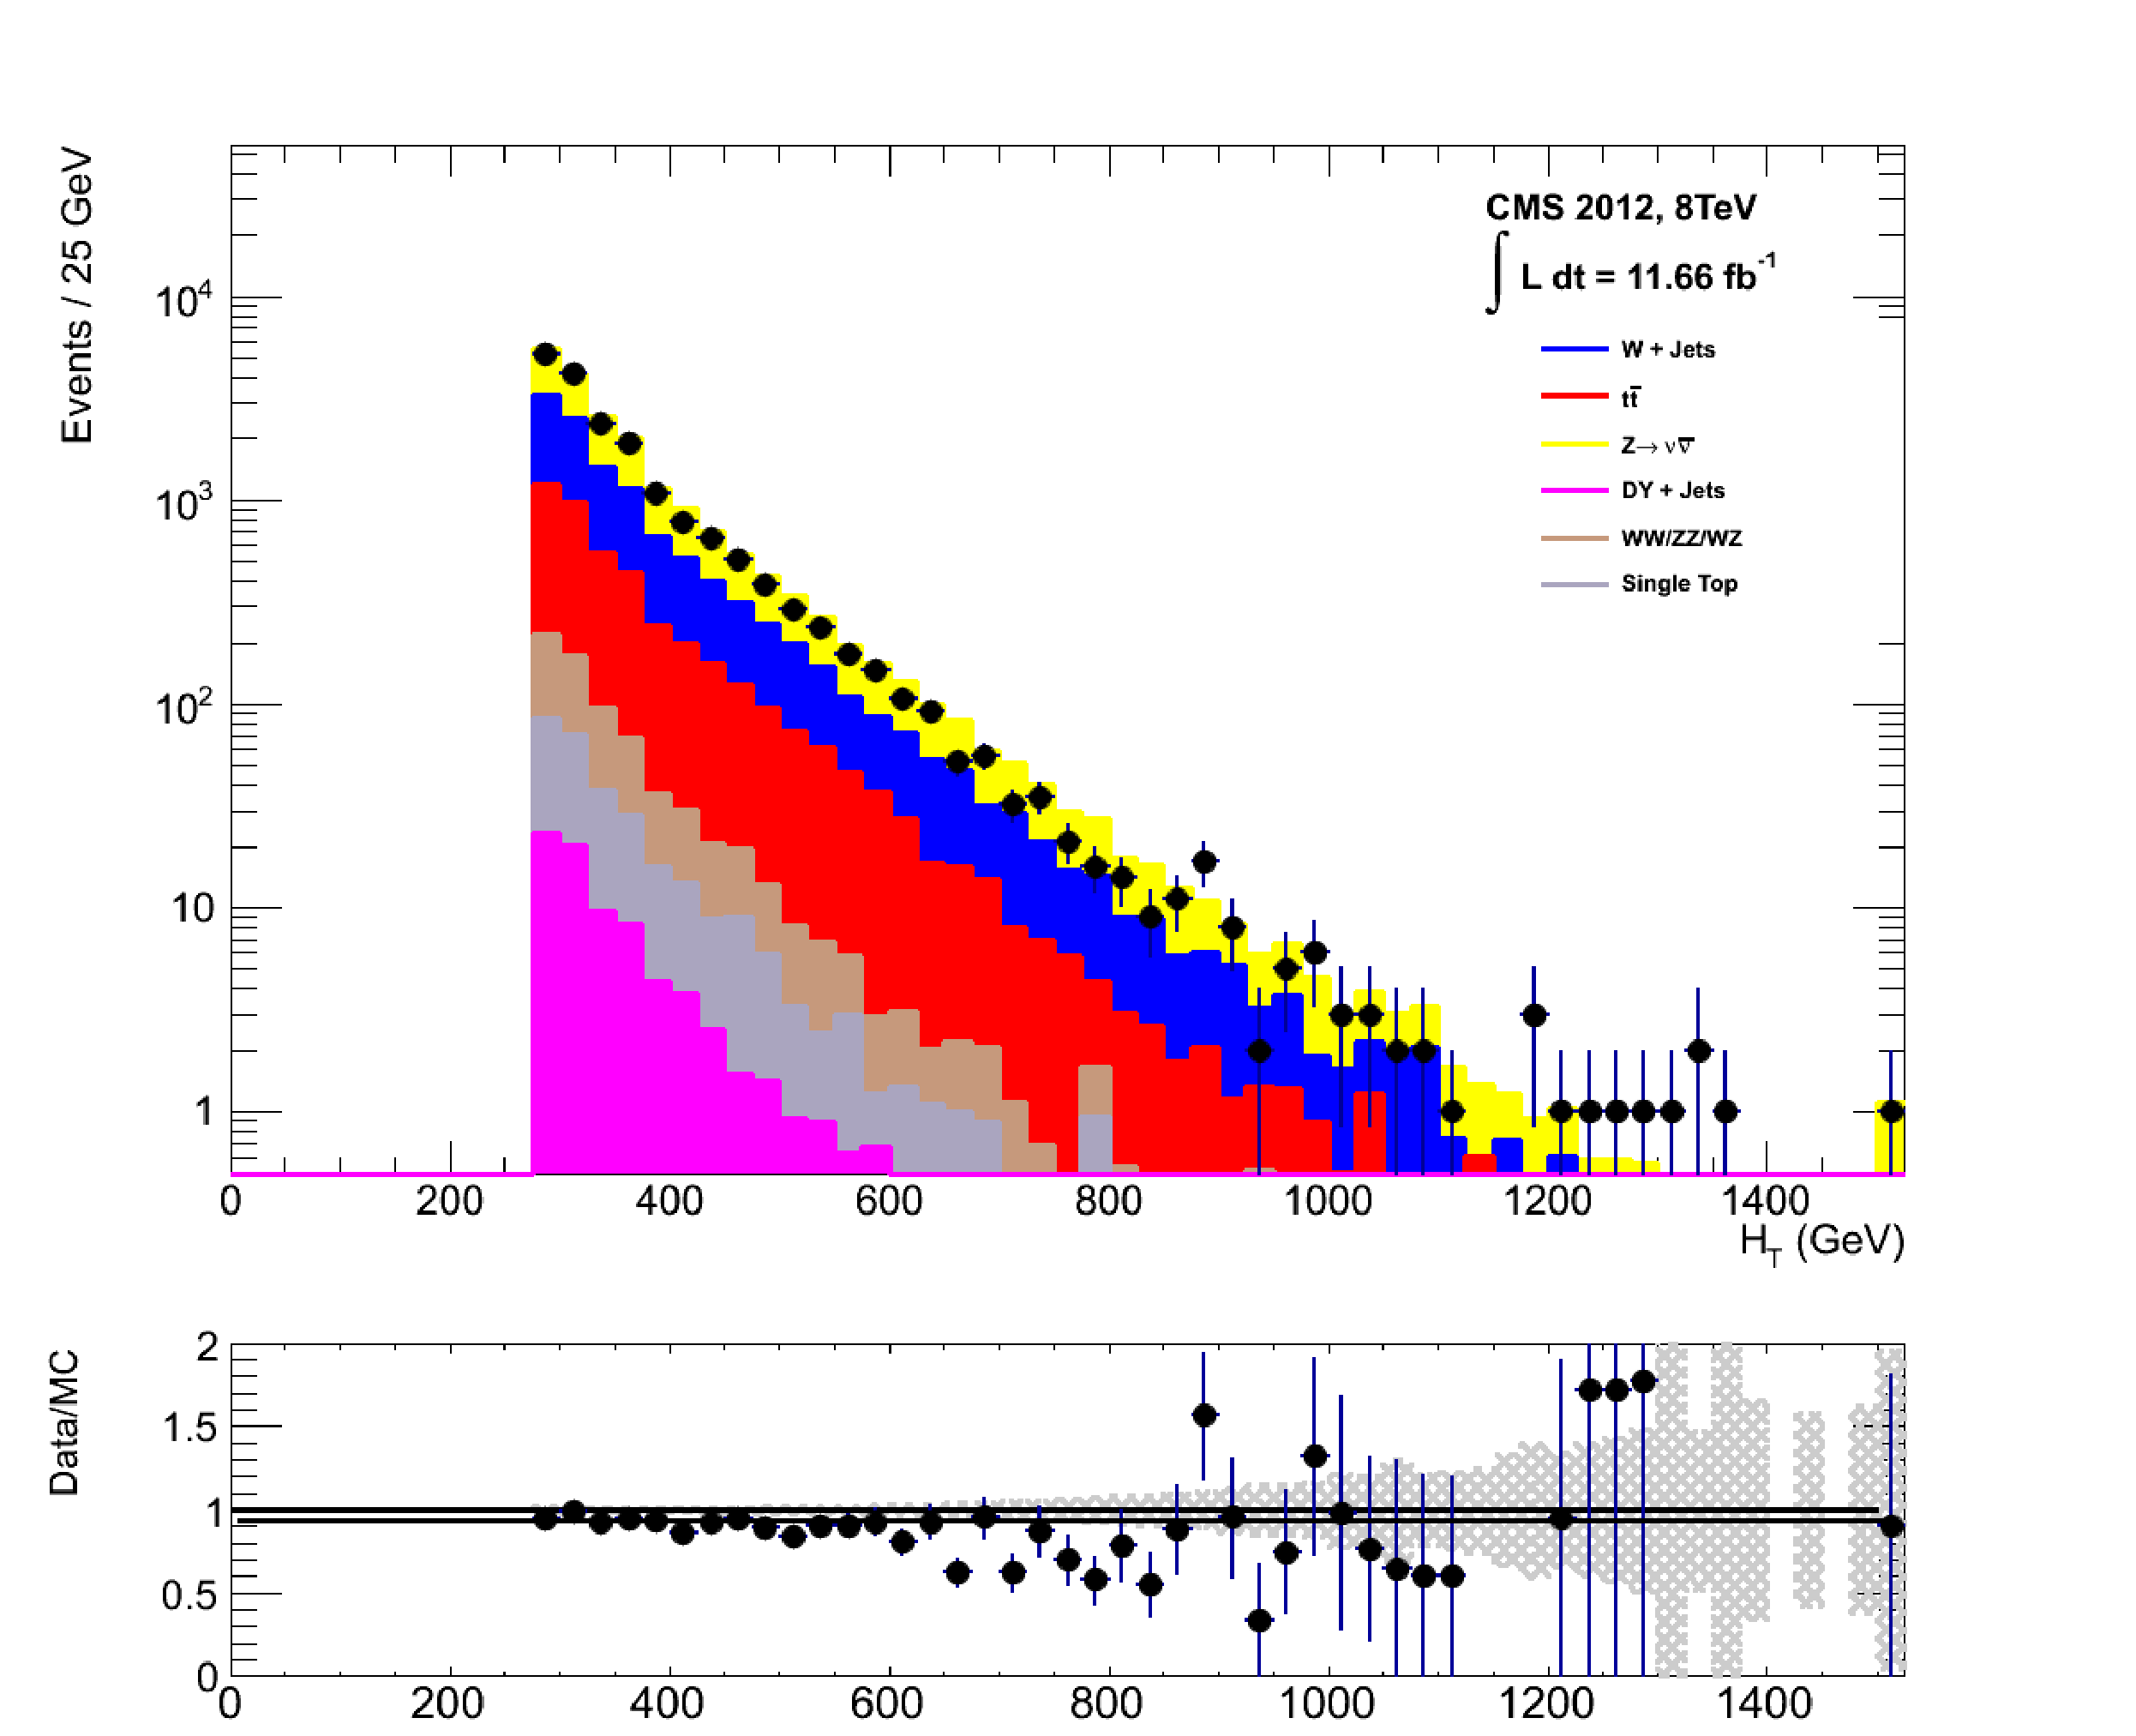
\includegraphics[width = 3.3in]{plots/had_ht_datamc.pdf}
(b) \theht
\end{minipage}
\begin{minipage}{.48\textwidth}
\centering
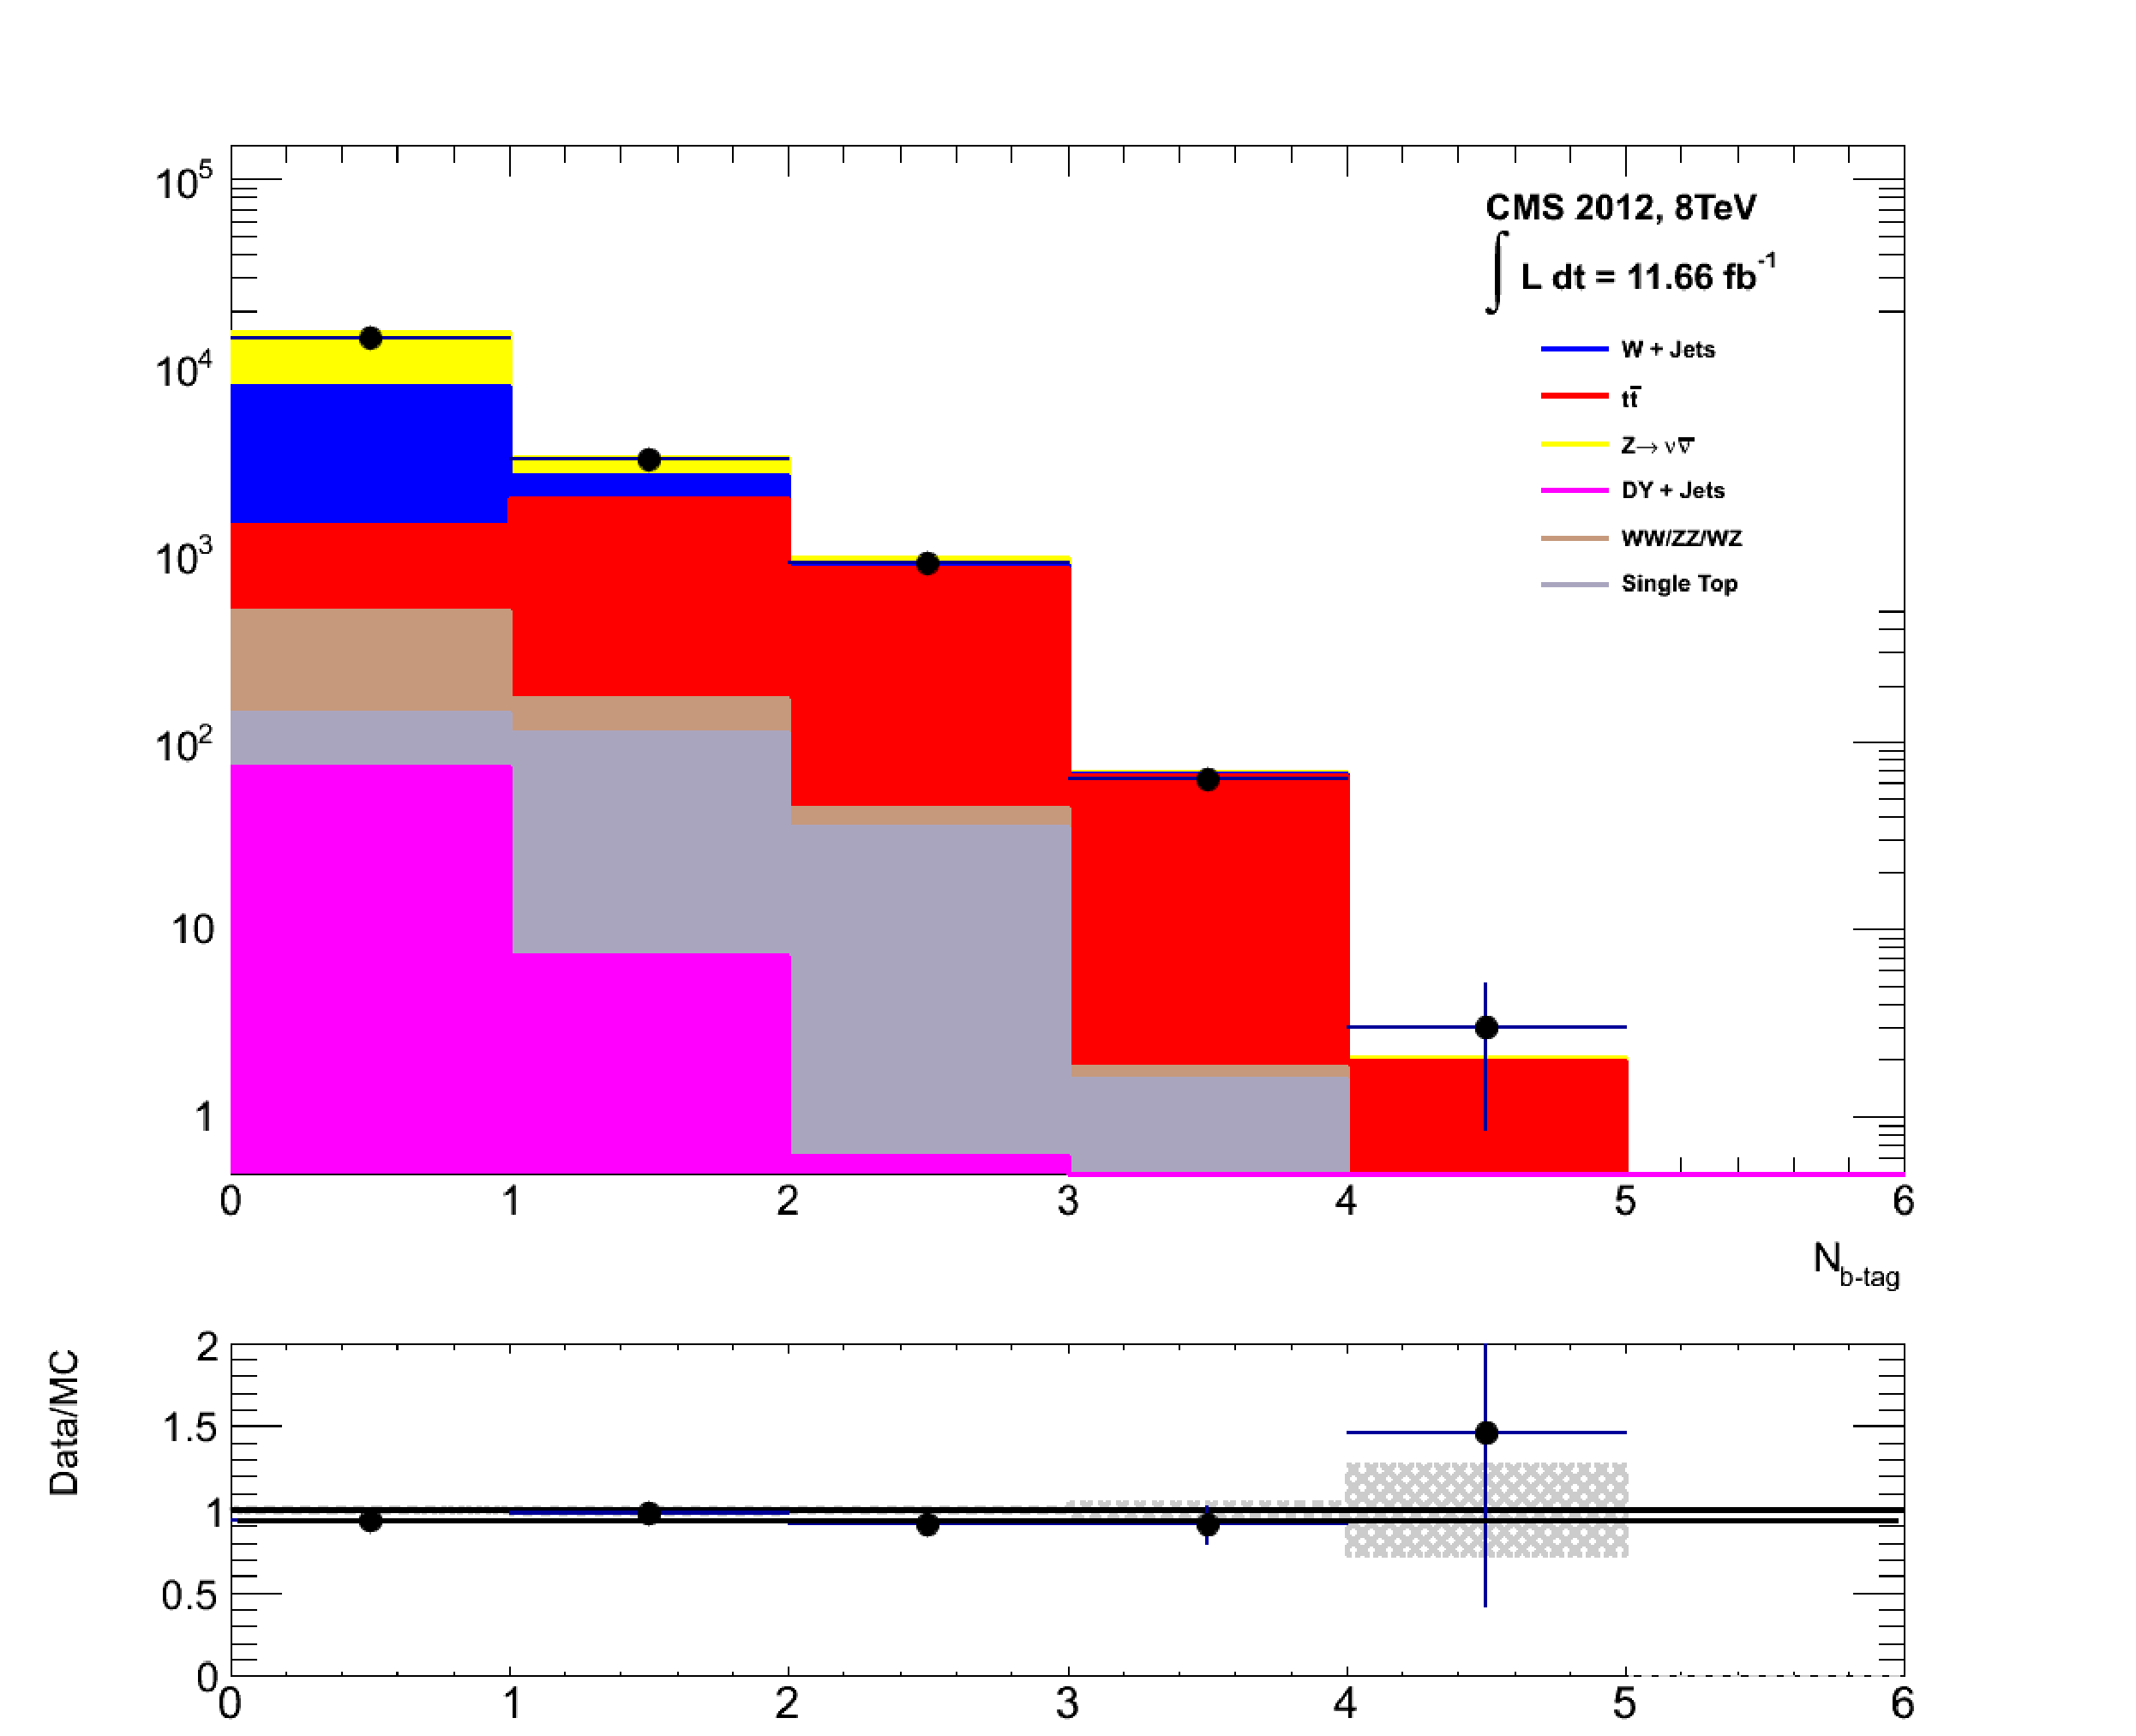
\includegraphics[width = 3.3in]{plots/had_nbtag_datamc.pdf}
$\text{(c}$) Btag Multiplicity
\end{minipage}
\begin{minipage}{.48\textwidth}
\centering
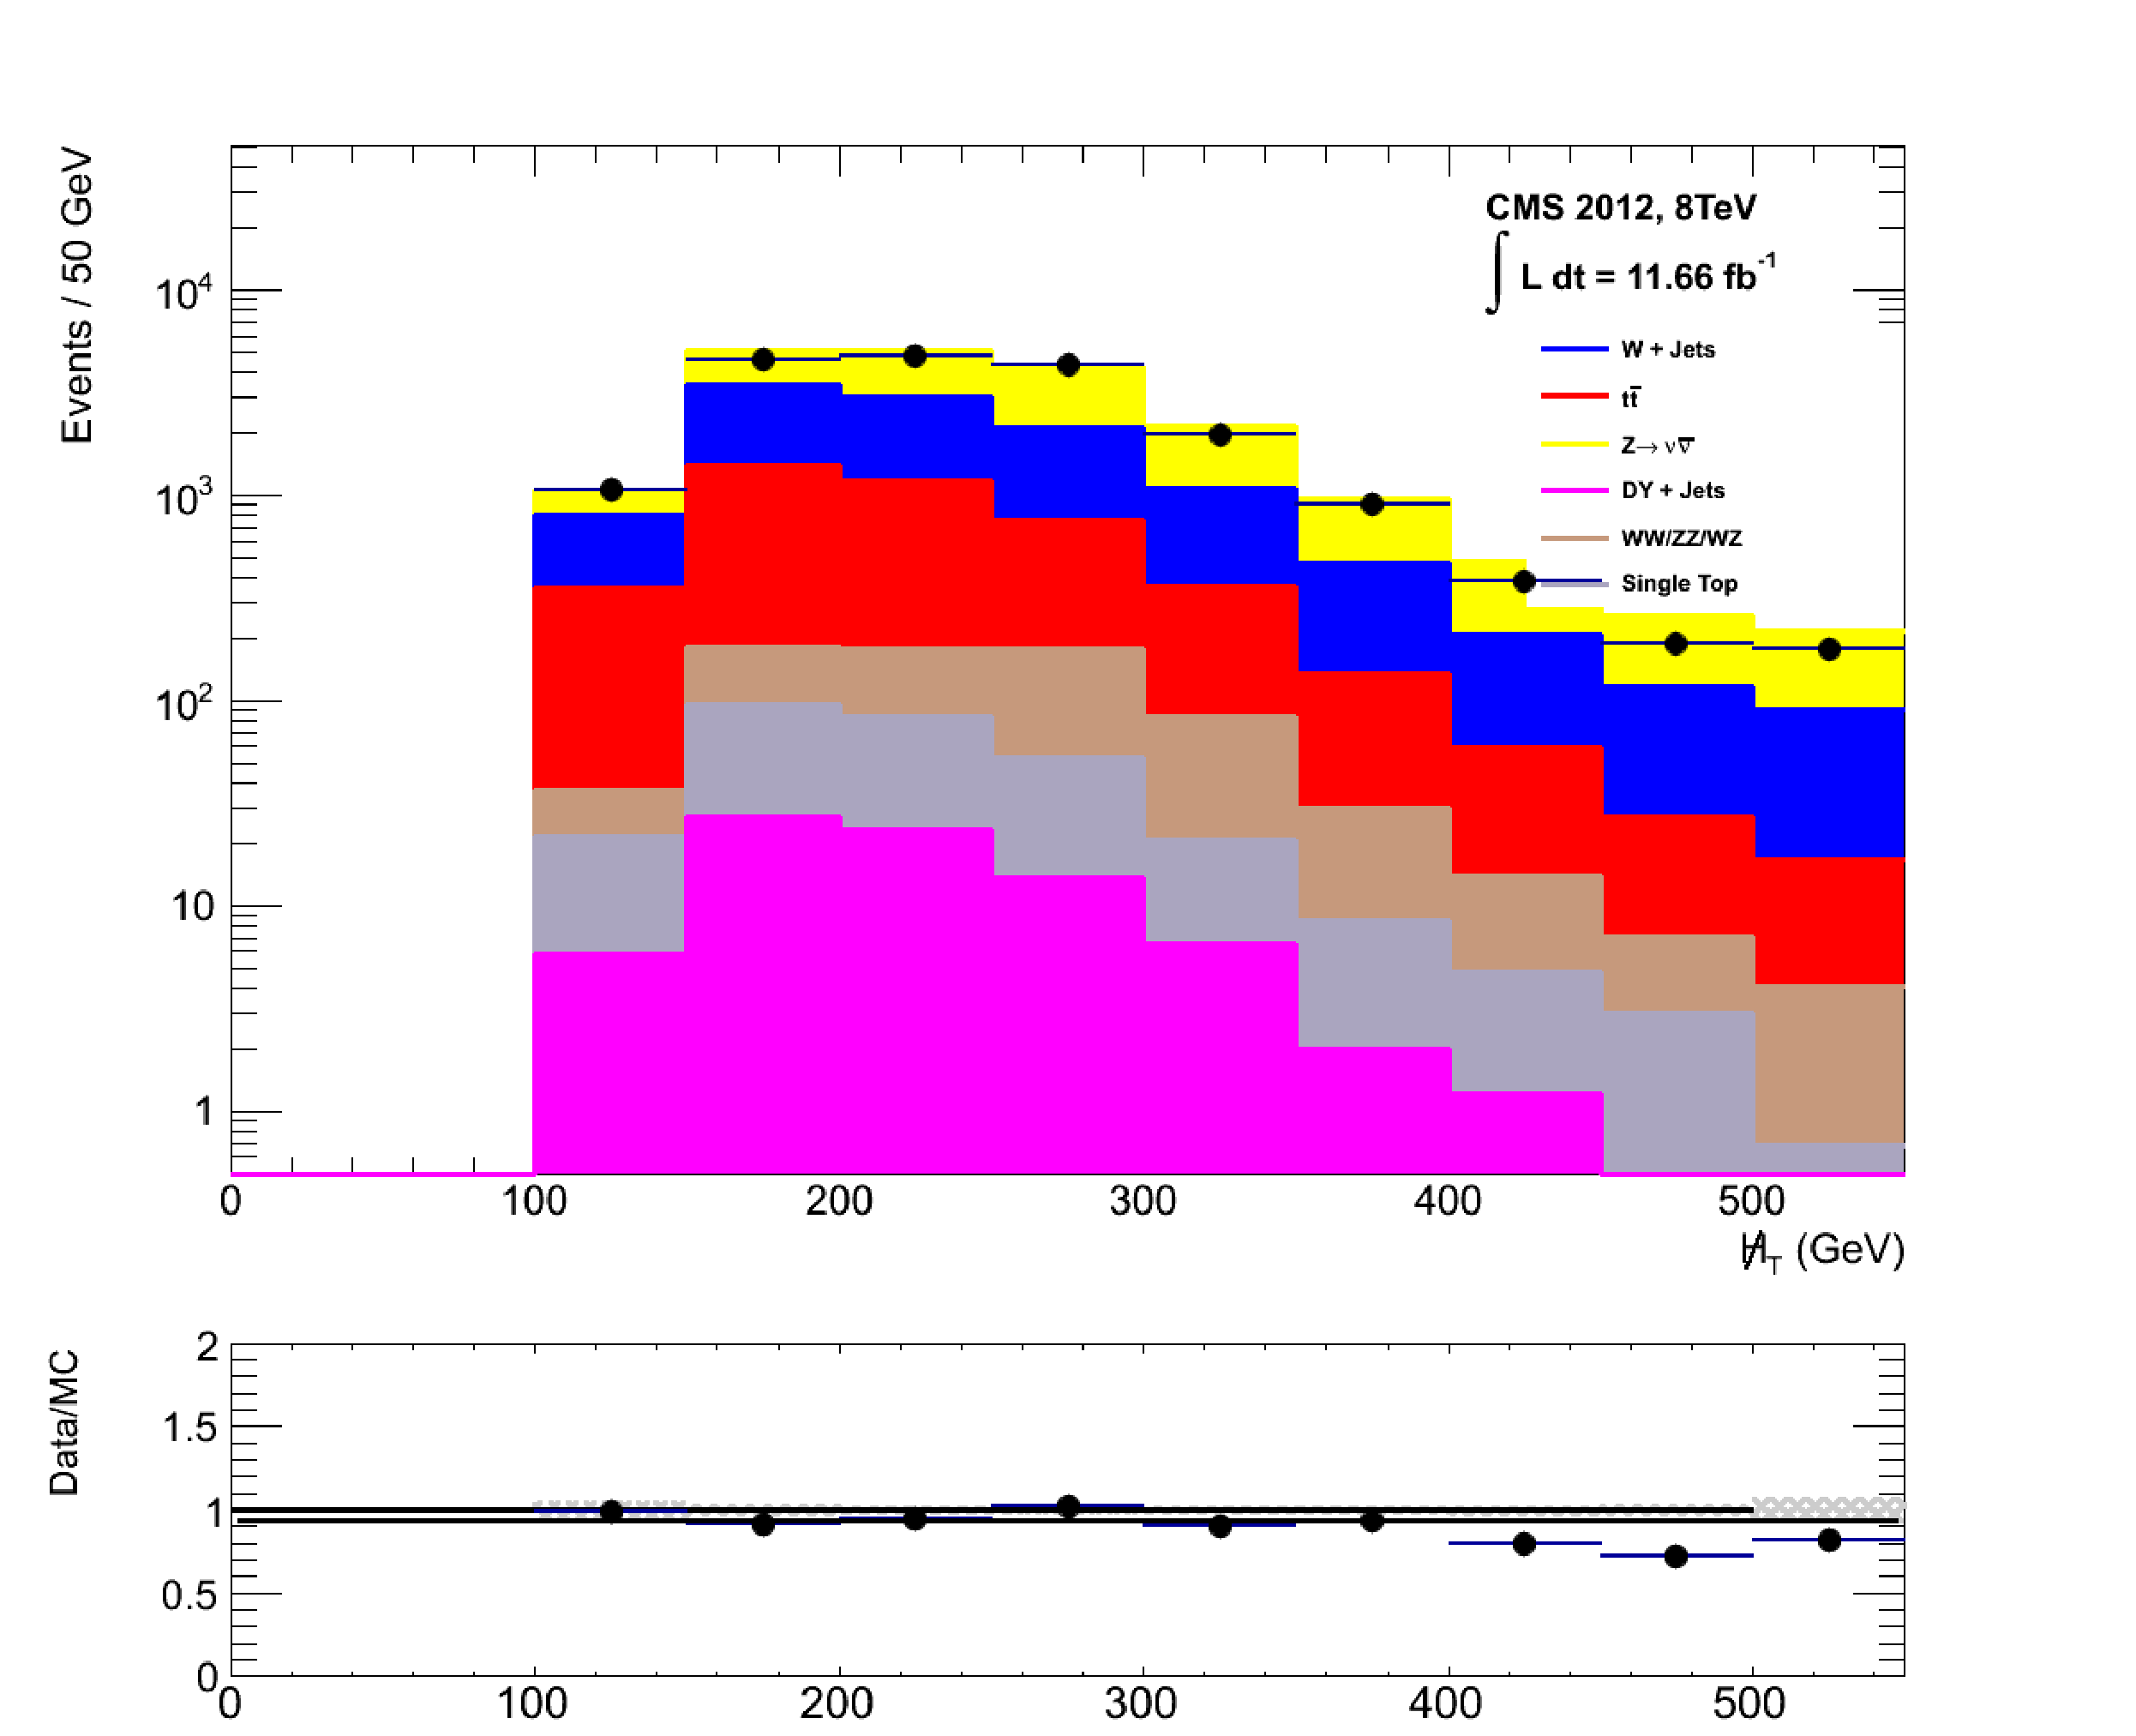
\includegraphics[width = 3.3in]{plots/had_mht_datamc.pdf}
(d) \mht
\end{minipage}
\captionof{figure}[Data/MC comparisons of key variables for the hadronic signal region.]{Data/MC comparisons of key variables for the hadronic signal region,following the application of the hadronic selection criteria and the requirements of \theht $>$ 275 \GeV and \alphat $>$ 0.55. Bands represent the uncertainties due to the statistical size of the MC samples. No requirement is made upon the number of b-tagged jets or jet multiplicity in these distributions.}\label{fig:hadmcplots}
\end{minipage}

\subsection{Control Sample Definition and Background Estimation}
\label{subsec:controlsampledefinition}

The method used to estimate the background contributions in the hadronic signal region relies on the use of a \acf{TF}. This is determined from MC simulation in both the control, $\text{N}_{\text{MC}}^{\text{control}}$, and signal, $\text{N}_{\text{MC}}^{\text{signal}}$, region to transform the observed yield measured in data for a control sample,  $\text{N}_{\text{obs}}^{\text{control}}$, into a background prediction, $\text{N}_{\text{pred}}^{\text{signal}}$, via Equation (\ref{eq:transfactor}),

\begin{equation}
\label{eq:transfactor}
\text{N}_{\text{pred}}^{\text{signal}} = \frac{\text{N}_{\text{MC}}^{\text{signal}}}{ \text{N}_{\text{MC}}^{\text{control}}} \times  \text{N}_{\text{obs}}^{\text{control}}.
\end{equation}

All MC samples are normalised to the luminosity of the data samples, 11.7 \fb. Through this method, ``vanilla'' predictions for the \ac{SM} background in the signal region can be made by considering separately the sum of the prediction from either the \mupjets and \gpjets or \mupjets and \dimupjets samples. However the final background estimation from which results are interpreted, is calculated via a fitting procedure defined formally by the likelihood model described in Chapter \ref{chap:SUSYresults}. 

The sum of the expected yields from all MC processes, in each control sample enter the denominator, $\text{N}_{\text{MC}}^{\text{control}}$  , of the \ac{TF} defined in Eq (\ref{eq:transfactor}). However for the numerator , $\text{N}_{\text{MC}}^{\text{signal}}$, only the relevant processes that the control sample is used in estimating a background for, enter into the \ac{TF}.

For the \mupjets sample the simulated MC processes which enter the numerator of the \ac{TF} are,

\begin{equation} 
\text{N}_{\text{MC}}^{\text{signal}}(\theht,n_{\text{jet}}) = N_{W} + N_{\ttbar} + N_{DY} + N_{t} + N_{di-boson},
\end{equation}

whilst for both the \dimupjets and \gpjets samples the only MC process used in the numerator is,

\begin{equation} 
\text{N}_{\text{MC}}^{\text{signal}}(\theht,n_{\text{jet}}) = N_{\zinv}.
\end{equation}

The control samples and the \ac{EWK} processes they are specifically tuned to select are defined below, with distributions of key variables for each of the control samples shown for illustrative purposes in Figures \ref{fig:muonmcplots}, \ref{fig:dimuonmcplots} and \ref{fig:photonmcplots}. No requirement is placed upon the number of b-tagged jets or jet multiplicity in the distributions shown. The MC distributions highlight the background compositions of each control sample, where in general, good agreement is observed between data and simulation, giving confidence that the samples are well understood. The contribution from QCD multi-jet events is expected to be negligible : 

\begin{itemize} 

\item[] \textbf{The \mupjets control sample}

Events from W + jets and \ttbar processes enter into the hadronic signal sample due to unidentified leptons from acceptance or threshold effects and hadronic tau decays. These leptons originate from the decay of high \pt W bosons. 

The control samples specifically identifies $W \rightarrow \mu\bar{\nu}$ decays within the same phase-space of the signal region, where the muon is subsequently ignored in the calculation of event level variables, i.e. \theht, \mht, \alphat. All kinematic jet-based cuts are identical to those applied in the hadronic search region detailed in Section (\ref{subsec:eventselection}), with the same \theht, jet multiplicity and b-jet multiplicity binning described above.

\begin{itemize}
\item Muons originating from W boson decays are selected by requiring one tightly isolated muon defined in Table \ref{tab:muonidtable}, with a \pt $>$ 30 \GeV and \abeta $<$ 2.1. Both of these threshold arise from trigger restrictions.  
\item The transverse mass of the W candidate must satisfy \mt$(\mu,\met) <$ 30\GeV ( to suppress QCD multi-jet events). 
\item Events which contain a jet overlapping with a muon $\Delta \text{R}(\mu,\text{jet}) <$ 0.5 are vetoed to remove events from muons produced as part of a jet's hadronisation process. 
\item Events containing a second muon candidate which has failed id, but passed \pt and \abeta requirements, are checked to have an invariant mass that satisfies m$_{Z}$ - 25 $<$ M$_{\mu_{1}\mu_{2}} >$ m$_{Z}$ + 25, thus removing $Z \rightarrow \mu\mu$ contamination.
\end{itemize}


\begin{minipage}{\linewidth}
\centering
\begin{minipage}{.48\textwidth}
\centering
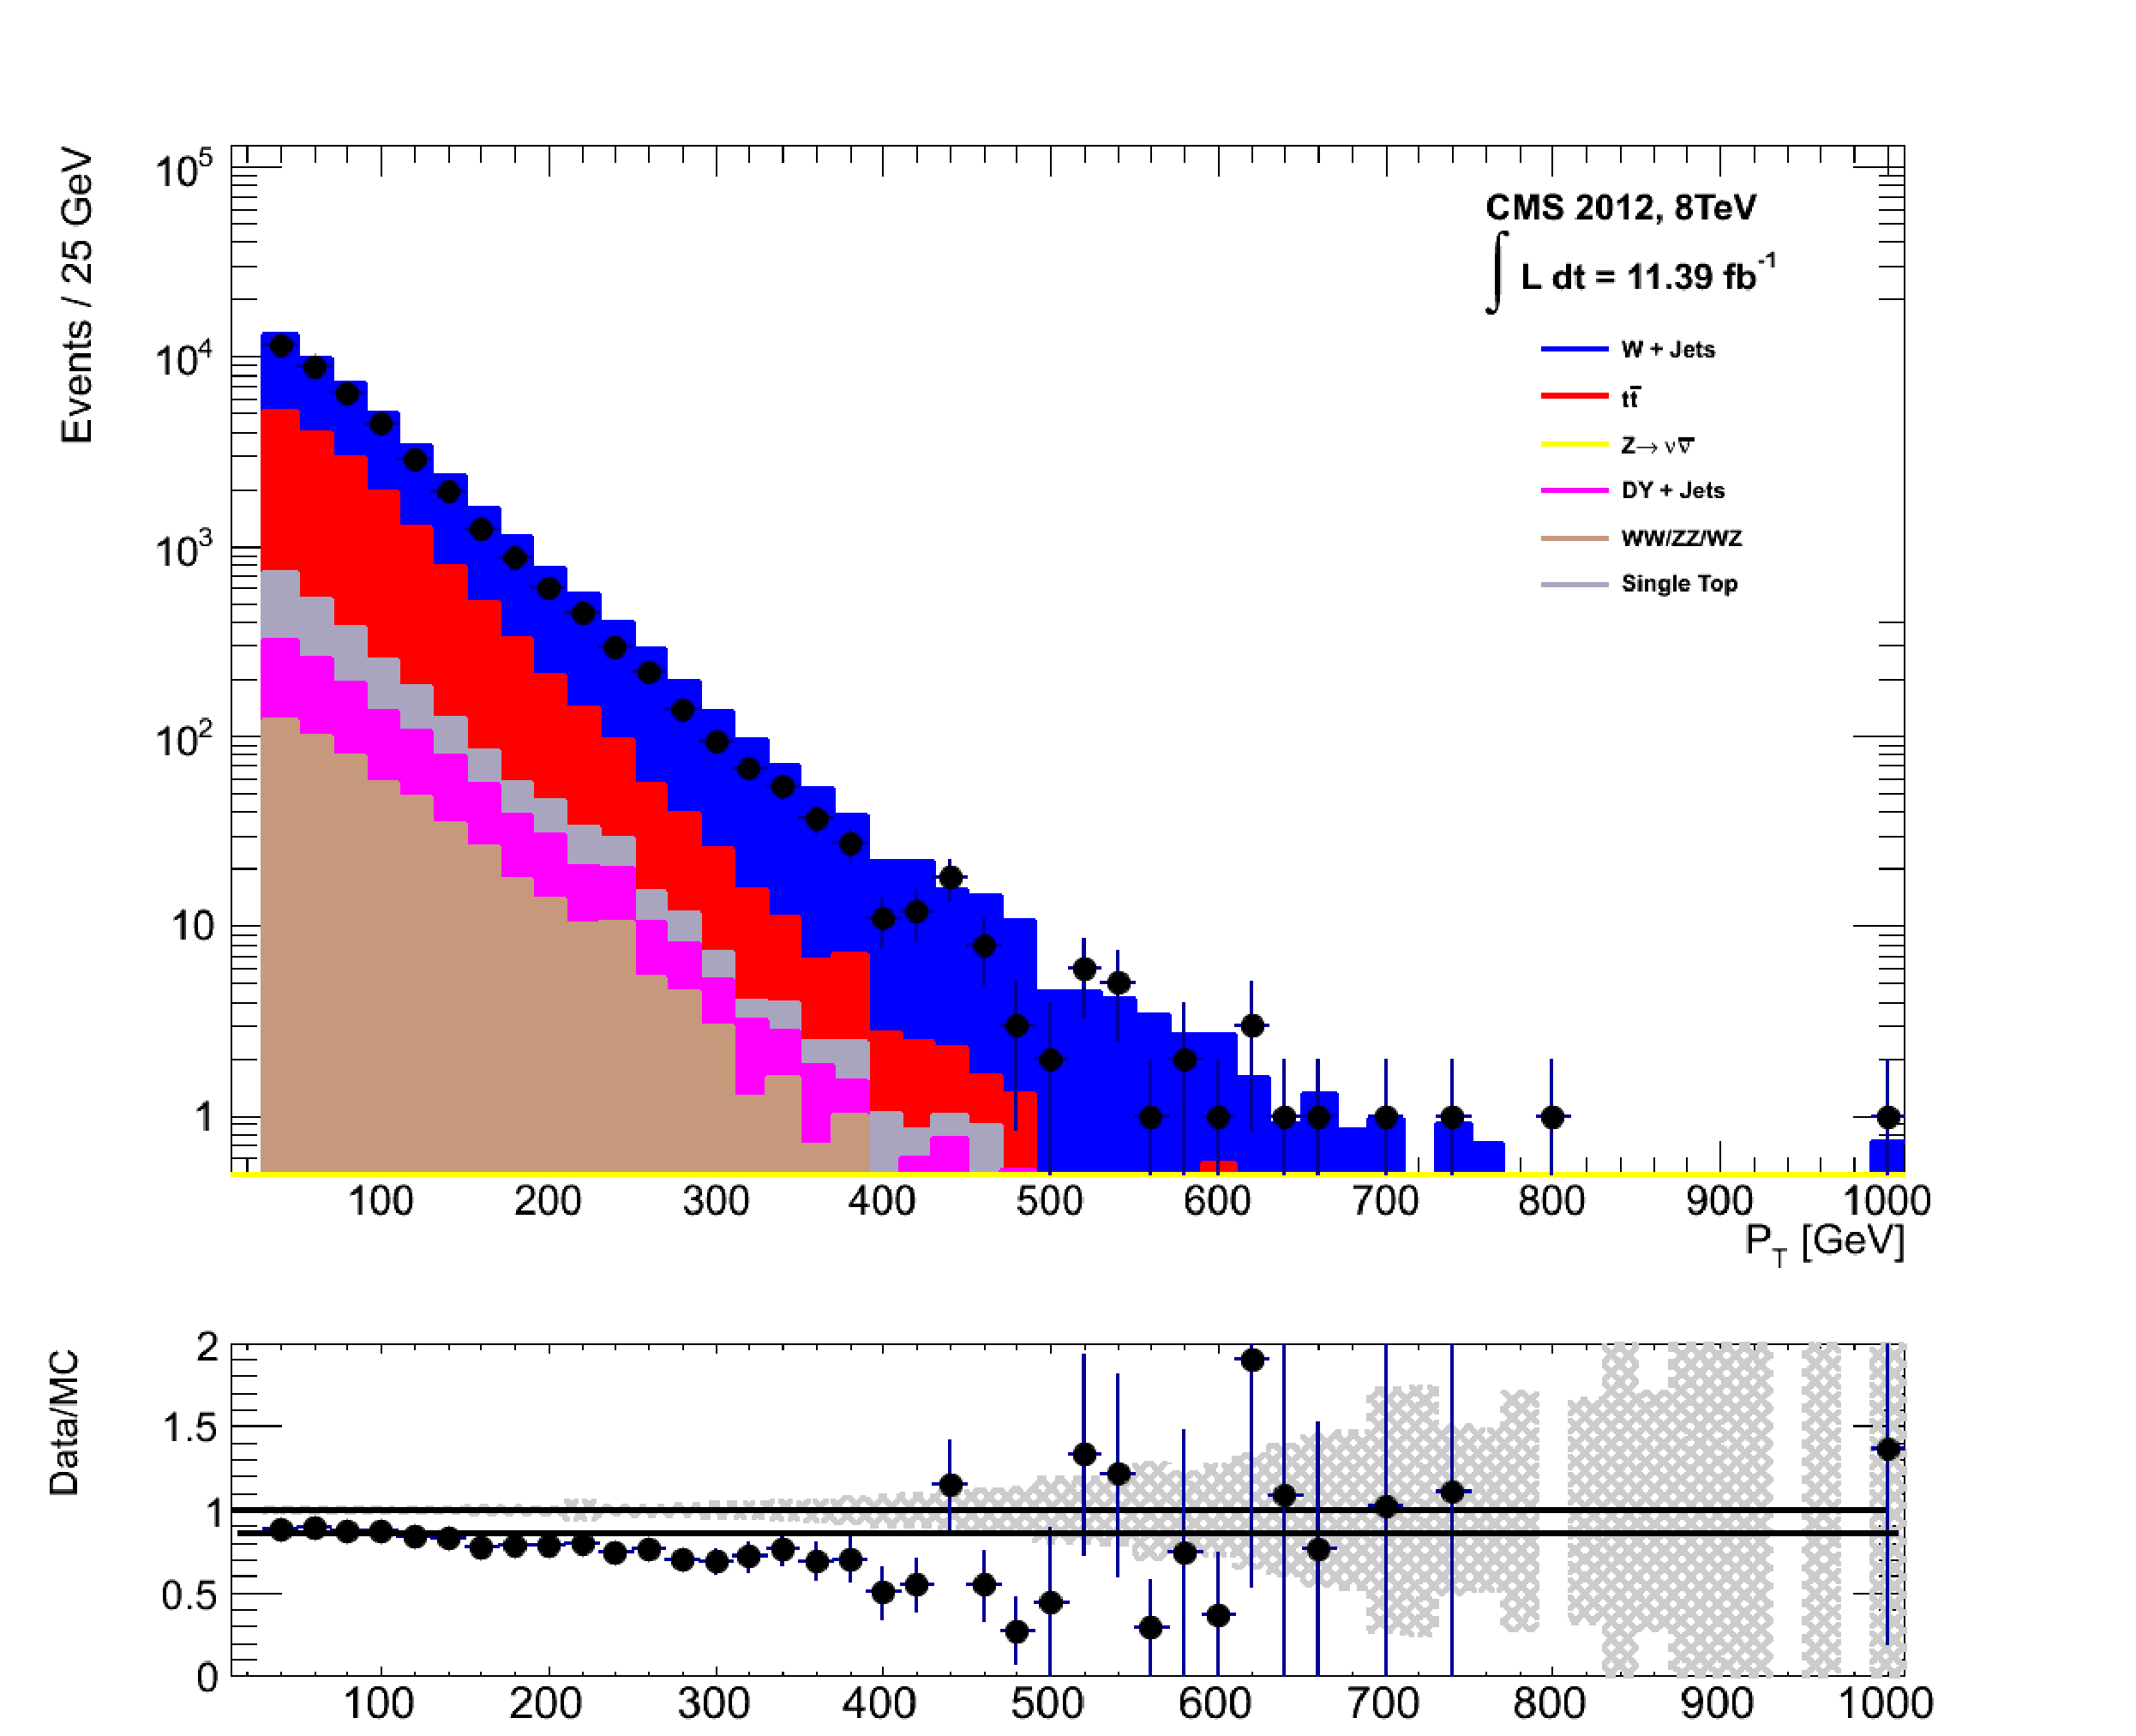
\includegraphics[width = 3.2in]{plots/muon_leadmu_datamc.pdf}
(a) Lead Muon \pt
\end{minipage}
\begin{minipage}{.48\textwidth}
\centering
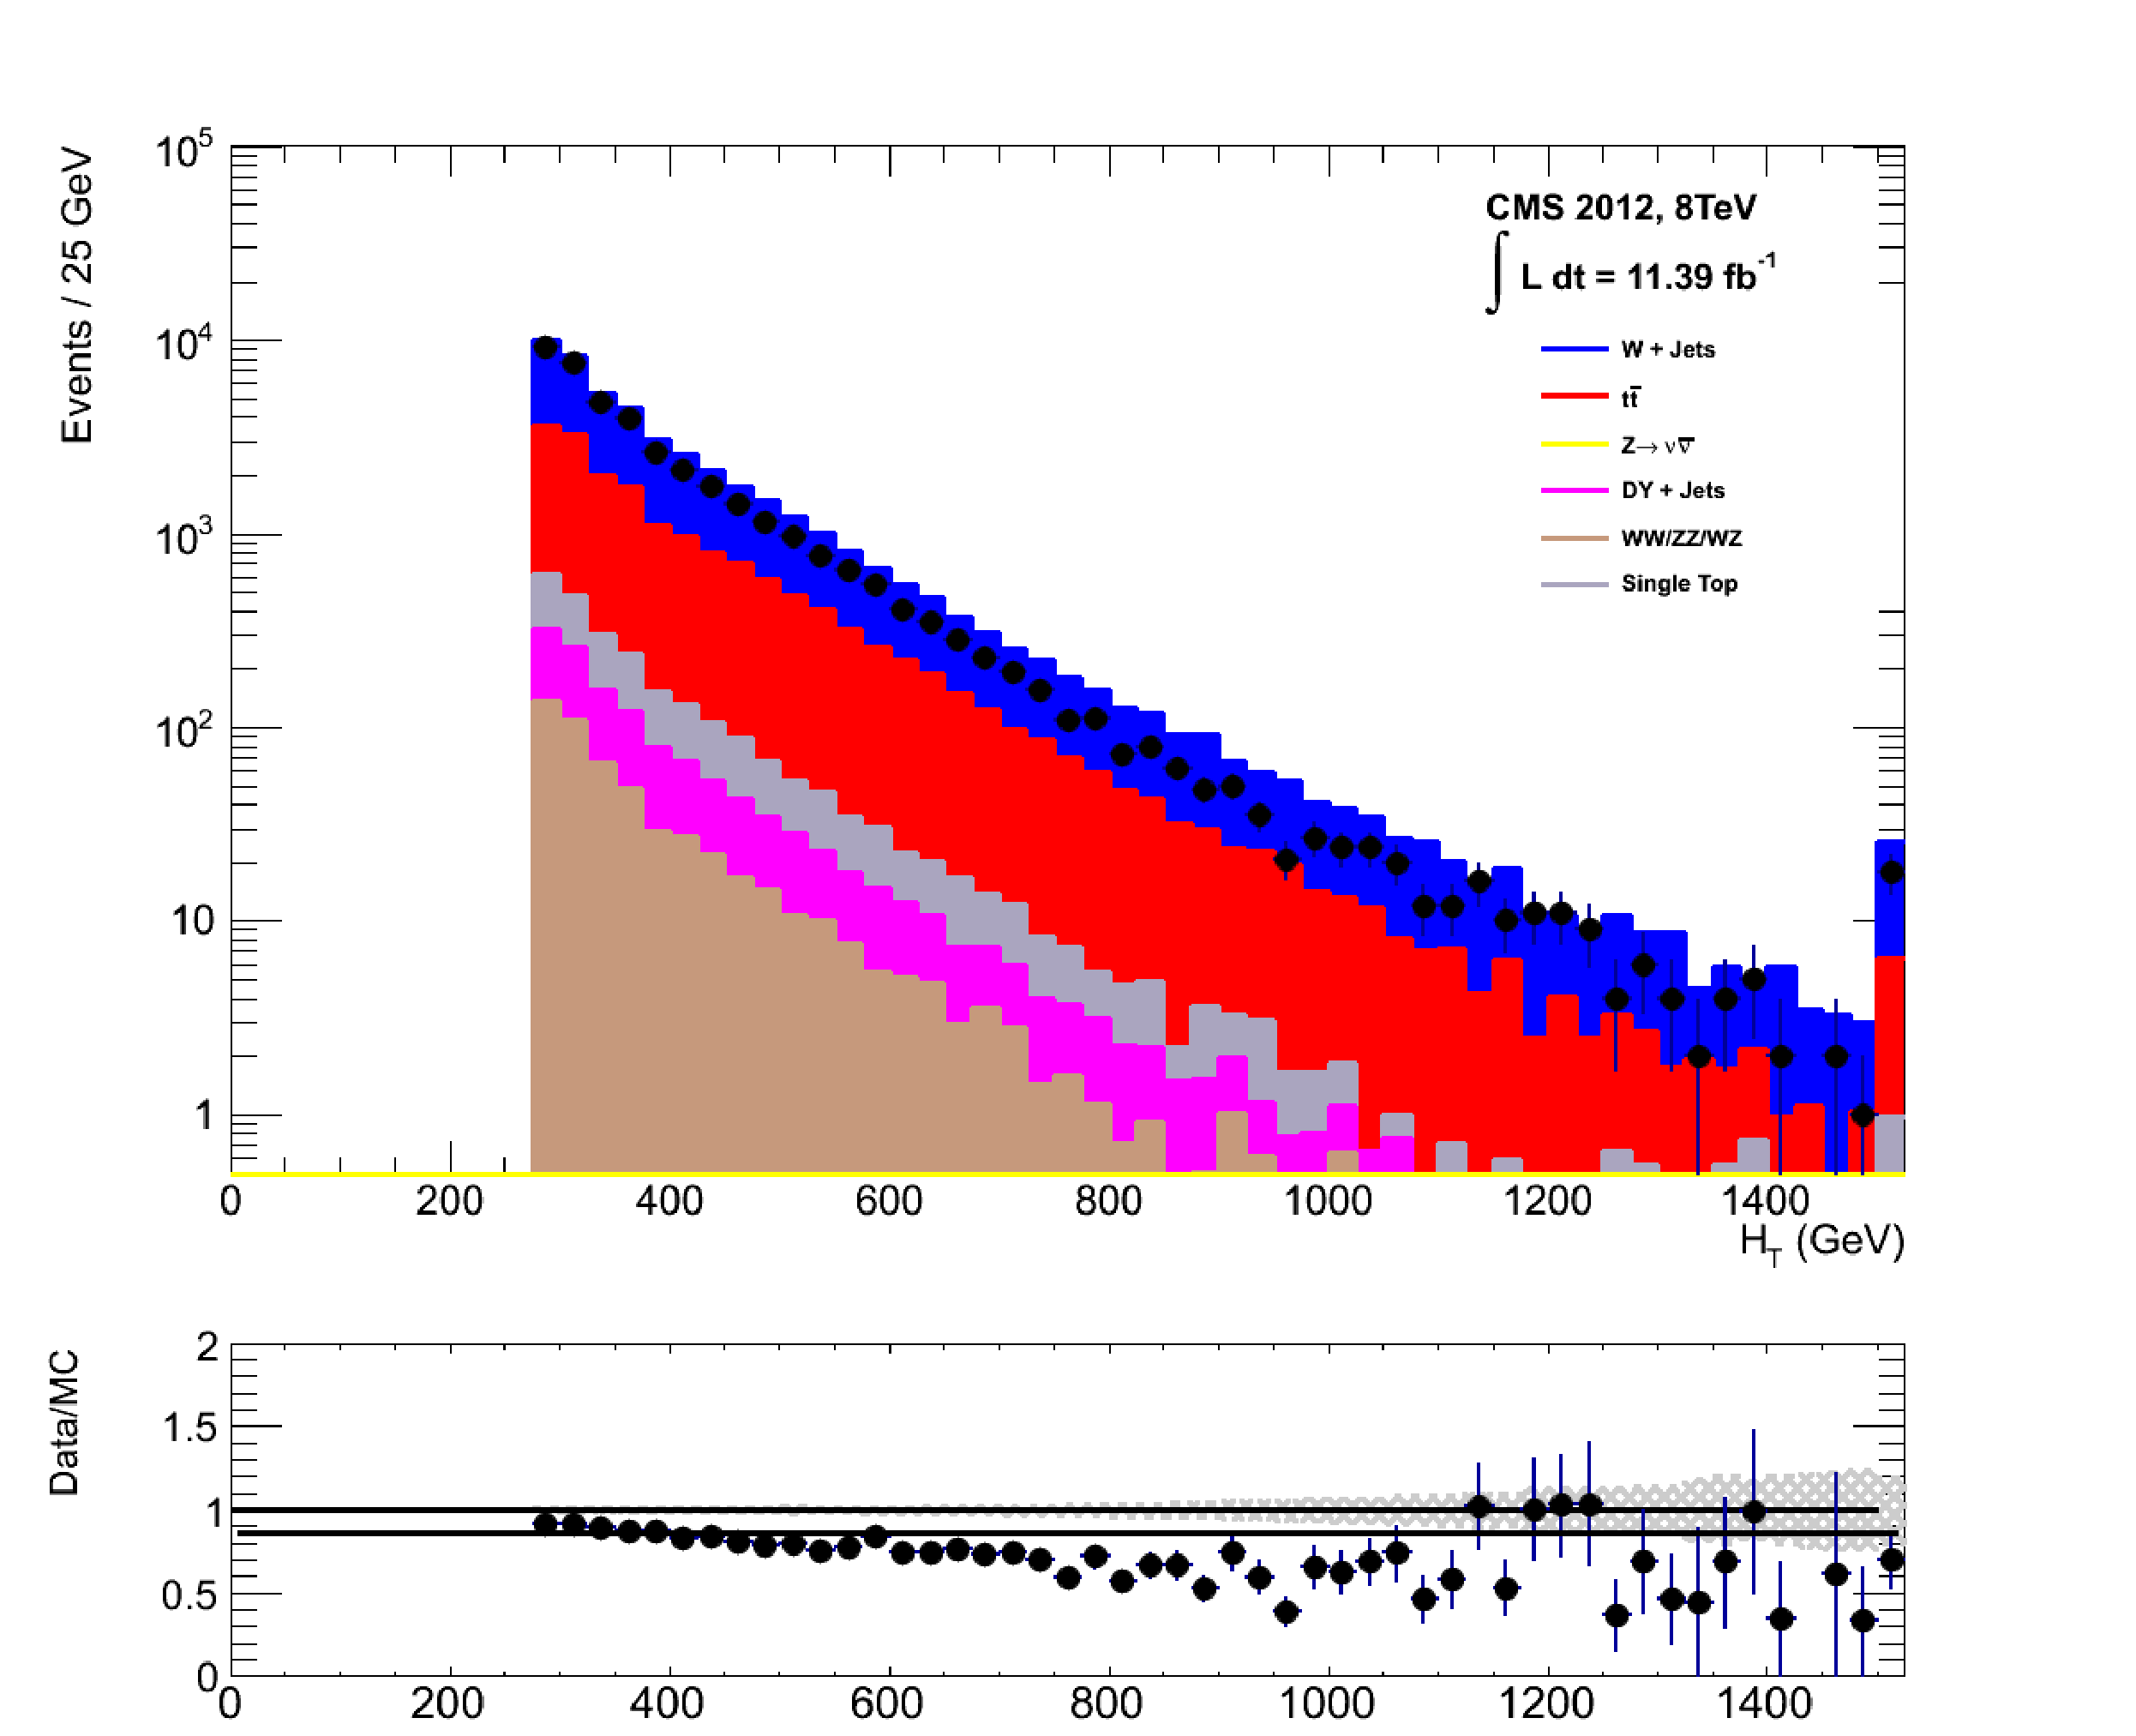
\includegraphics[width = 3.2in]{plots/muon_ht_datamc.pdf}
(b) \theht
\end{minipage}
\end{minipage}
\xspace
\begin{minipage}{\linewidth}
\centering
\begin{minipage}{.48\textwidth}
\centering
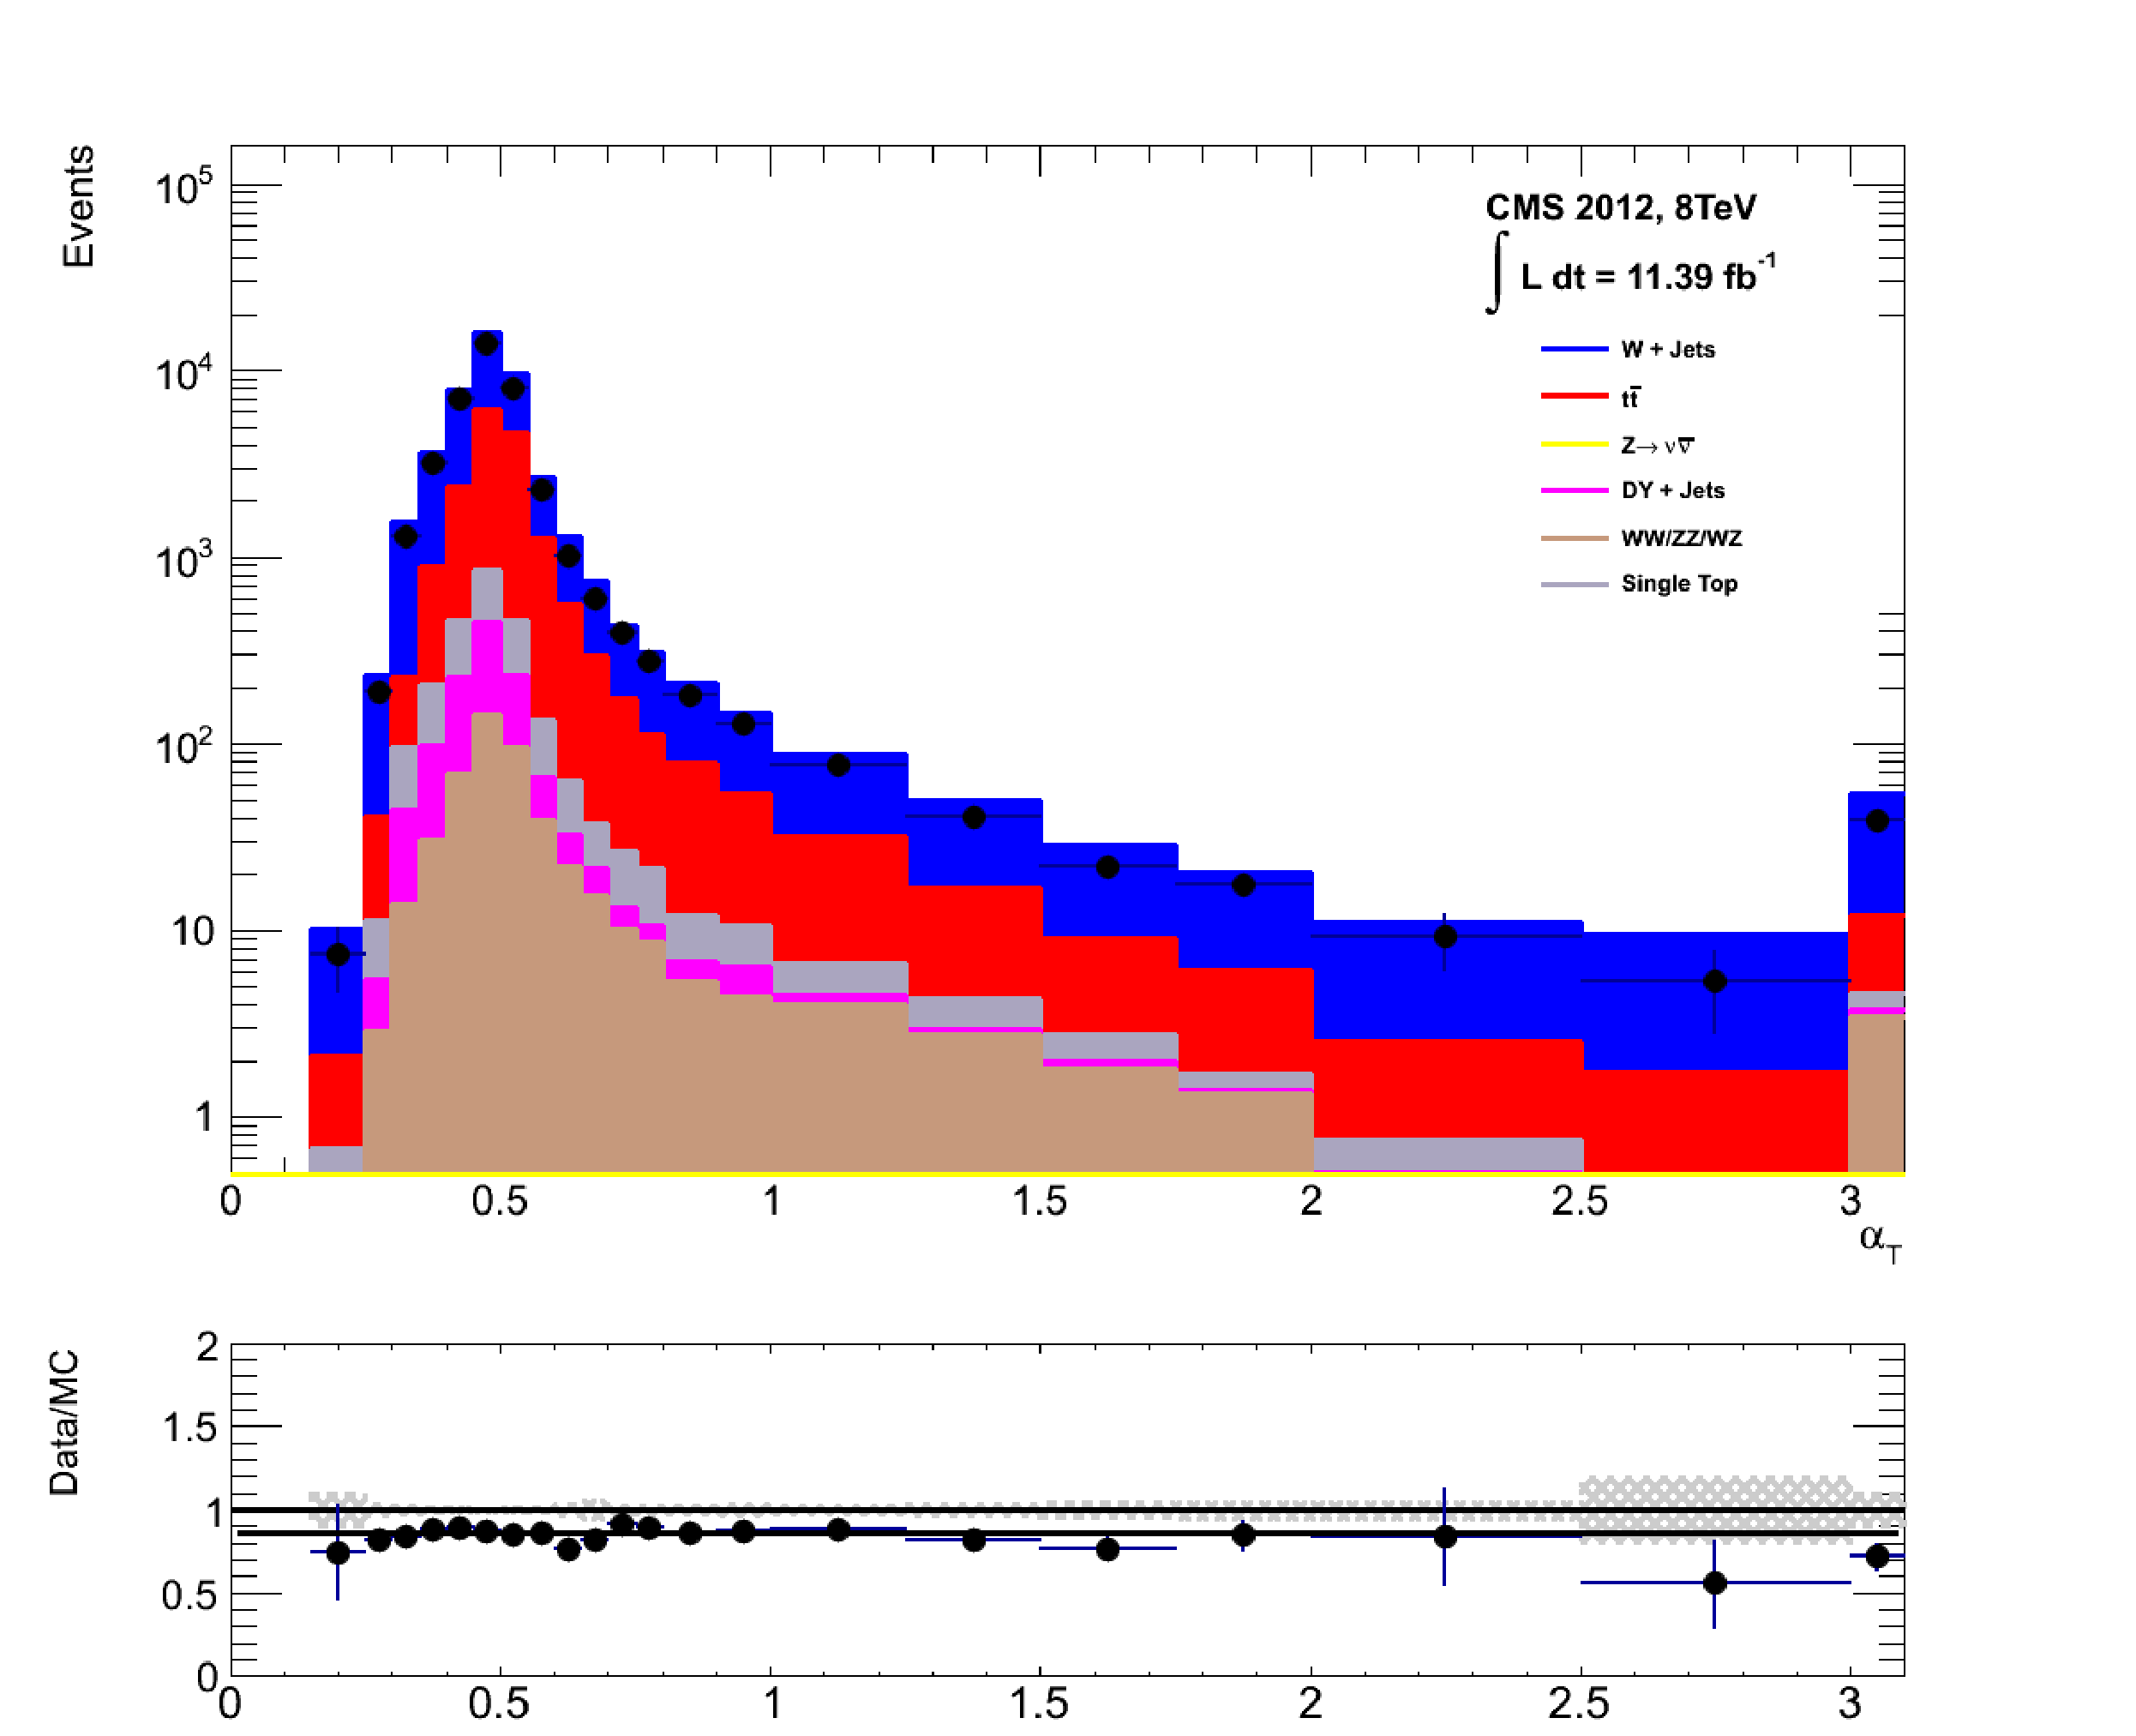
\includegraphics[width = 3.2in]{plots/muon_alphat_datamc.pdf}
$\text{(c}$) \alphat
\end{minipage}
\begin{minipage}{.48\textwidth}
\centering
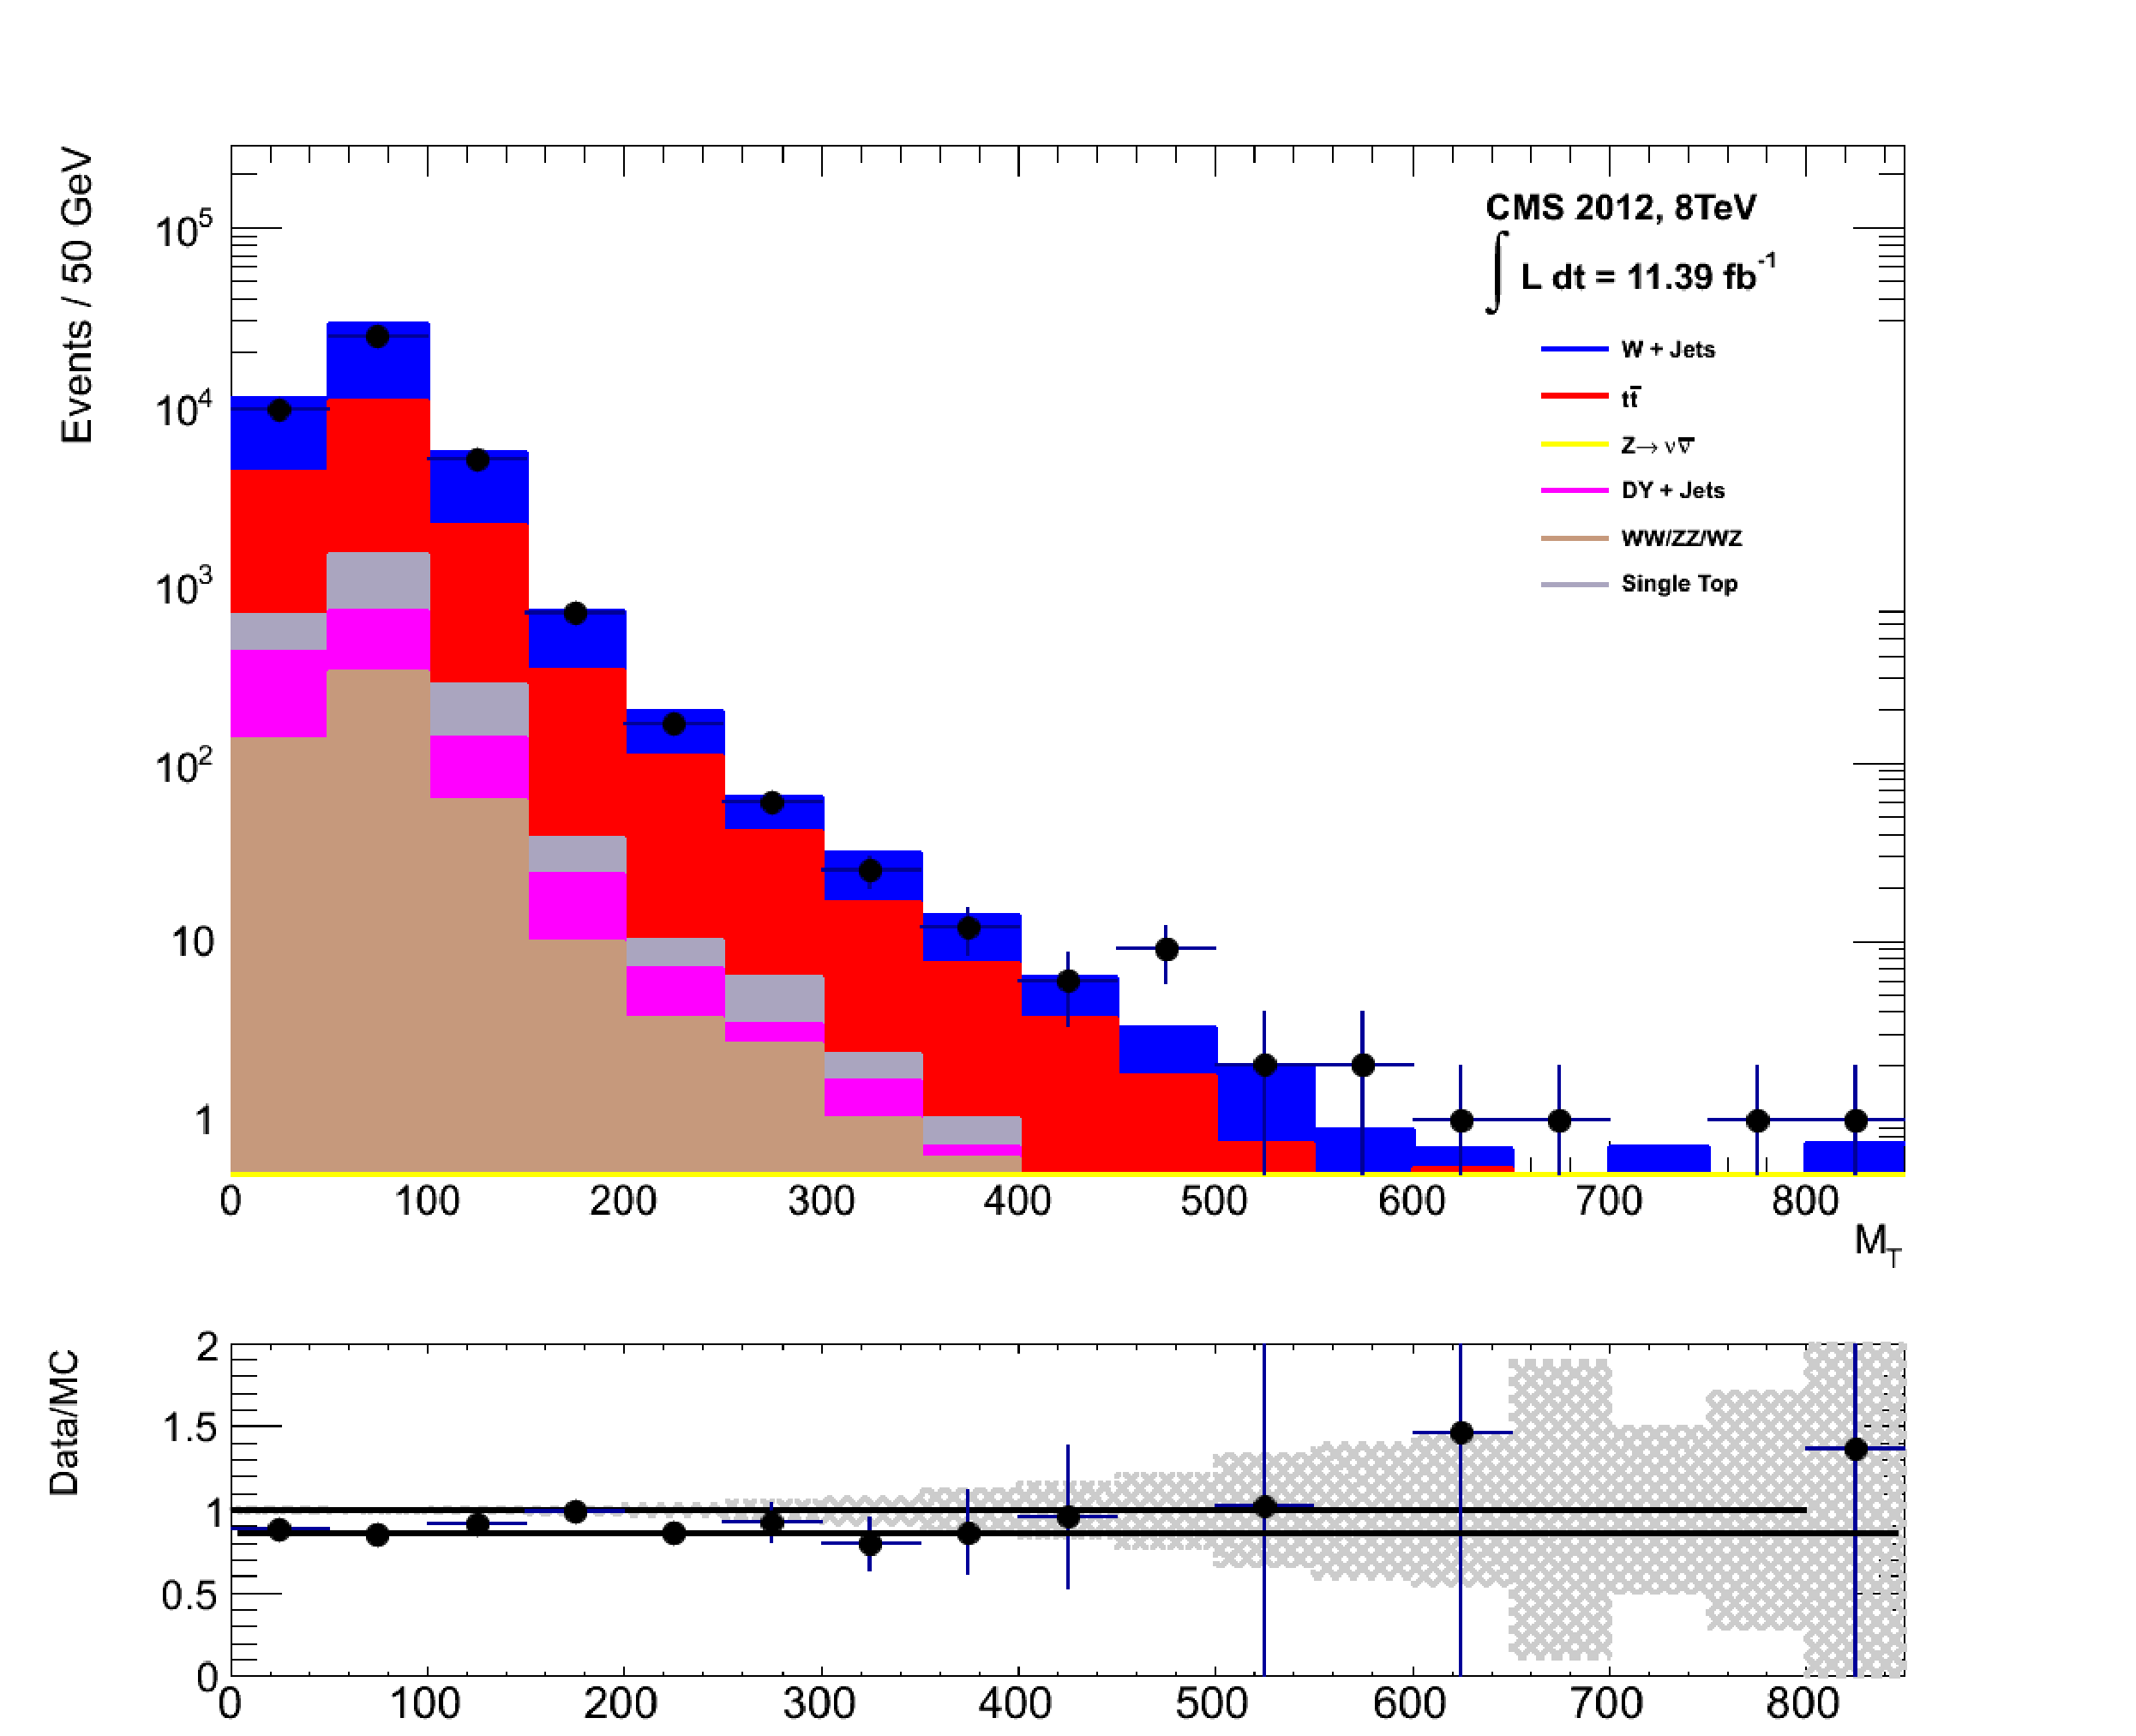
\includegraphics[width = 3.2in]{plots/muon_mt_datamc.pdf}
(d) Transverse mass $M_{T}$
\end{minipage}
\captionof{figure}[Data/MC comparisons of key variables for the \mupjets selection.]{Data/MC comparisons of key variables for the \mupjets selection,following the application of selection criteria and the requirements that \theht $>$ 275 \GeV. Bands represent the uncertainties due to the statistical size of the MC samples. No requirement is made upon the number of b-tagged jets or jet multiplicity in these distributions.}\label{fig:muonmcplots}
\end{minipage}

\item[] \textbf{The \dimupjets control sample}

The  \zinv + jets background enters into the signal region from genuine \met from the escaping neutrinos. This background is estimated using two control samples, the first of which is the \zmumu + jets process, which posses identical kinematic properties, but with different acceptance and branching ratio \cite{pdg2012}.

The same acceptance requirements as the \mupjets selection for muons is applied, as defined in Table  \ref{tab:muonidtable}. Muons  in the event are ignored for the purpose of the calculation of event level variables. Kinematic jet-based cuts and phase space binning identical to the hadronic search region are also applied.

\begin{itemize}
\item Muons origination from a Z boson decay are selected requiring exactly two tightly isolated muons. Due to trigger requirements the leading muon is required to have  \pt $>$ 30 \GeV and \abeta $<$ 2.1. The requirement of the \pt on the second muon is relaxed to 10 \GeV.
\item Events are vetoed if containing a jet overlapping with a muon $\Delta \text{R}(\mu,\text{jet}) <$ 0.5. 
\item In order to specifically select two muons both originating from a single Z boson decay, the invariant mass of the two muons must satisfy m$_{Z}$ - 25 $>$ M$_{\mu_{1}\mu_{2}} <$ m$_{Z}$ + 25. 
\end{itemize}

The \dimupjets sample is used to make predictions in the signal region in the two lowest \theht bins, providing coverage where the \gpjets sample is unable to, due to trigger requirements. In higher \theht bins, the higher statistics of the \gpjets sample is instead used to determine the \zinv estimation.

\begin{minipage}{\linewidth}
\centering
\begin{minipage}{.48\textwidth}
\centering
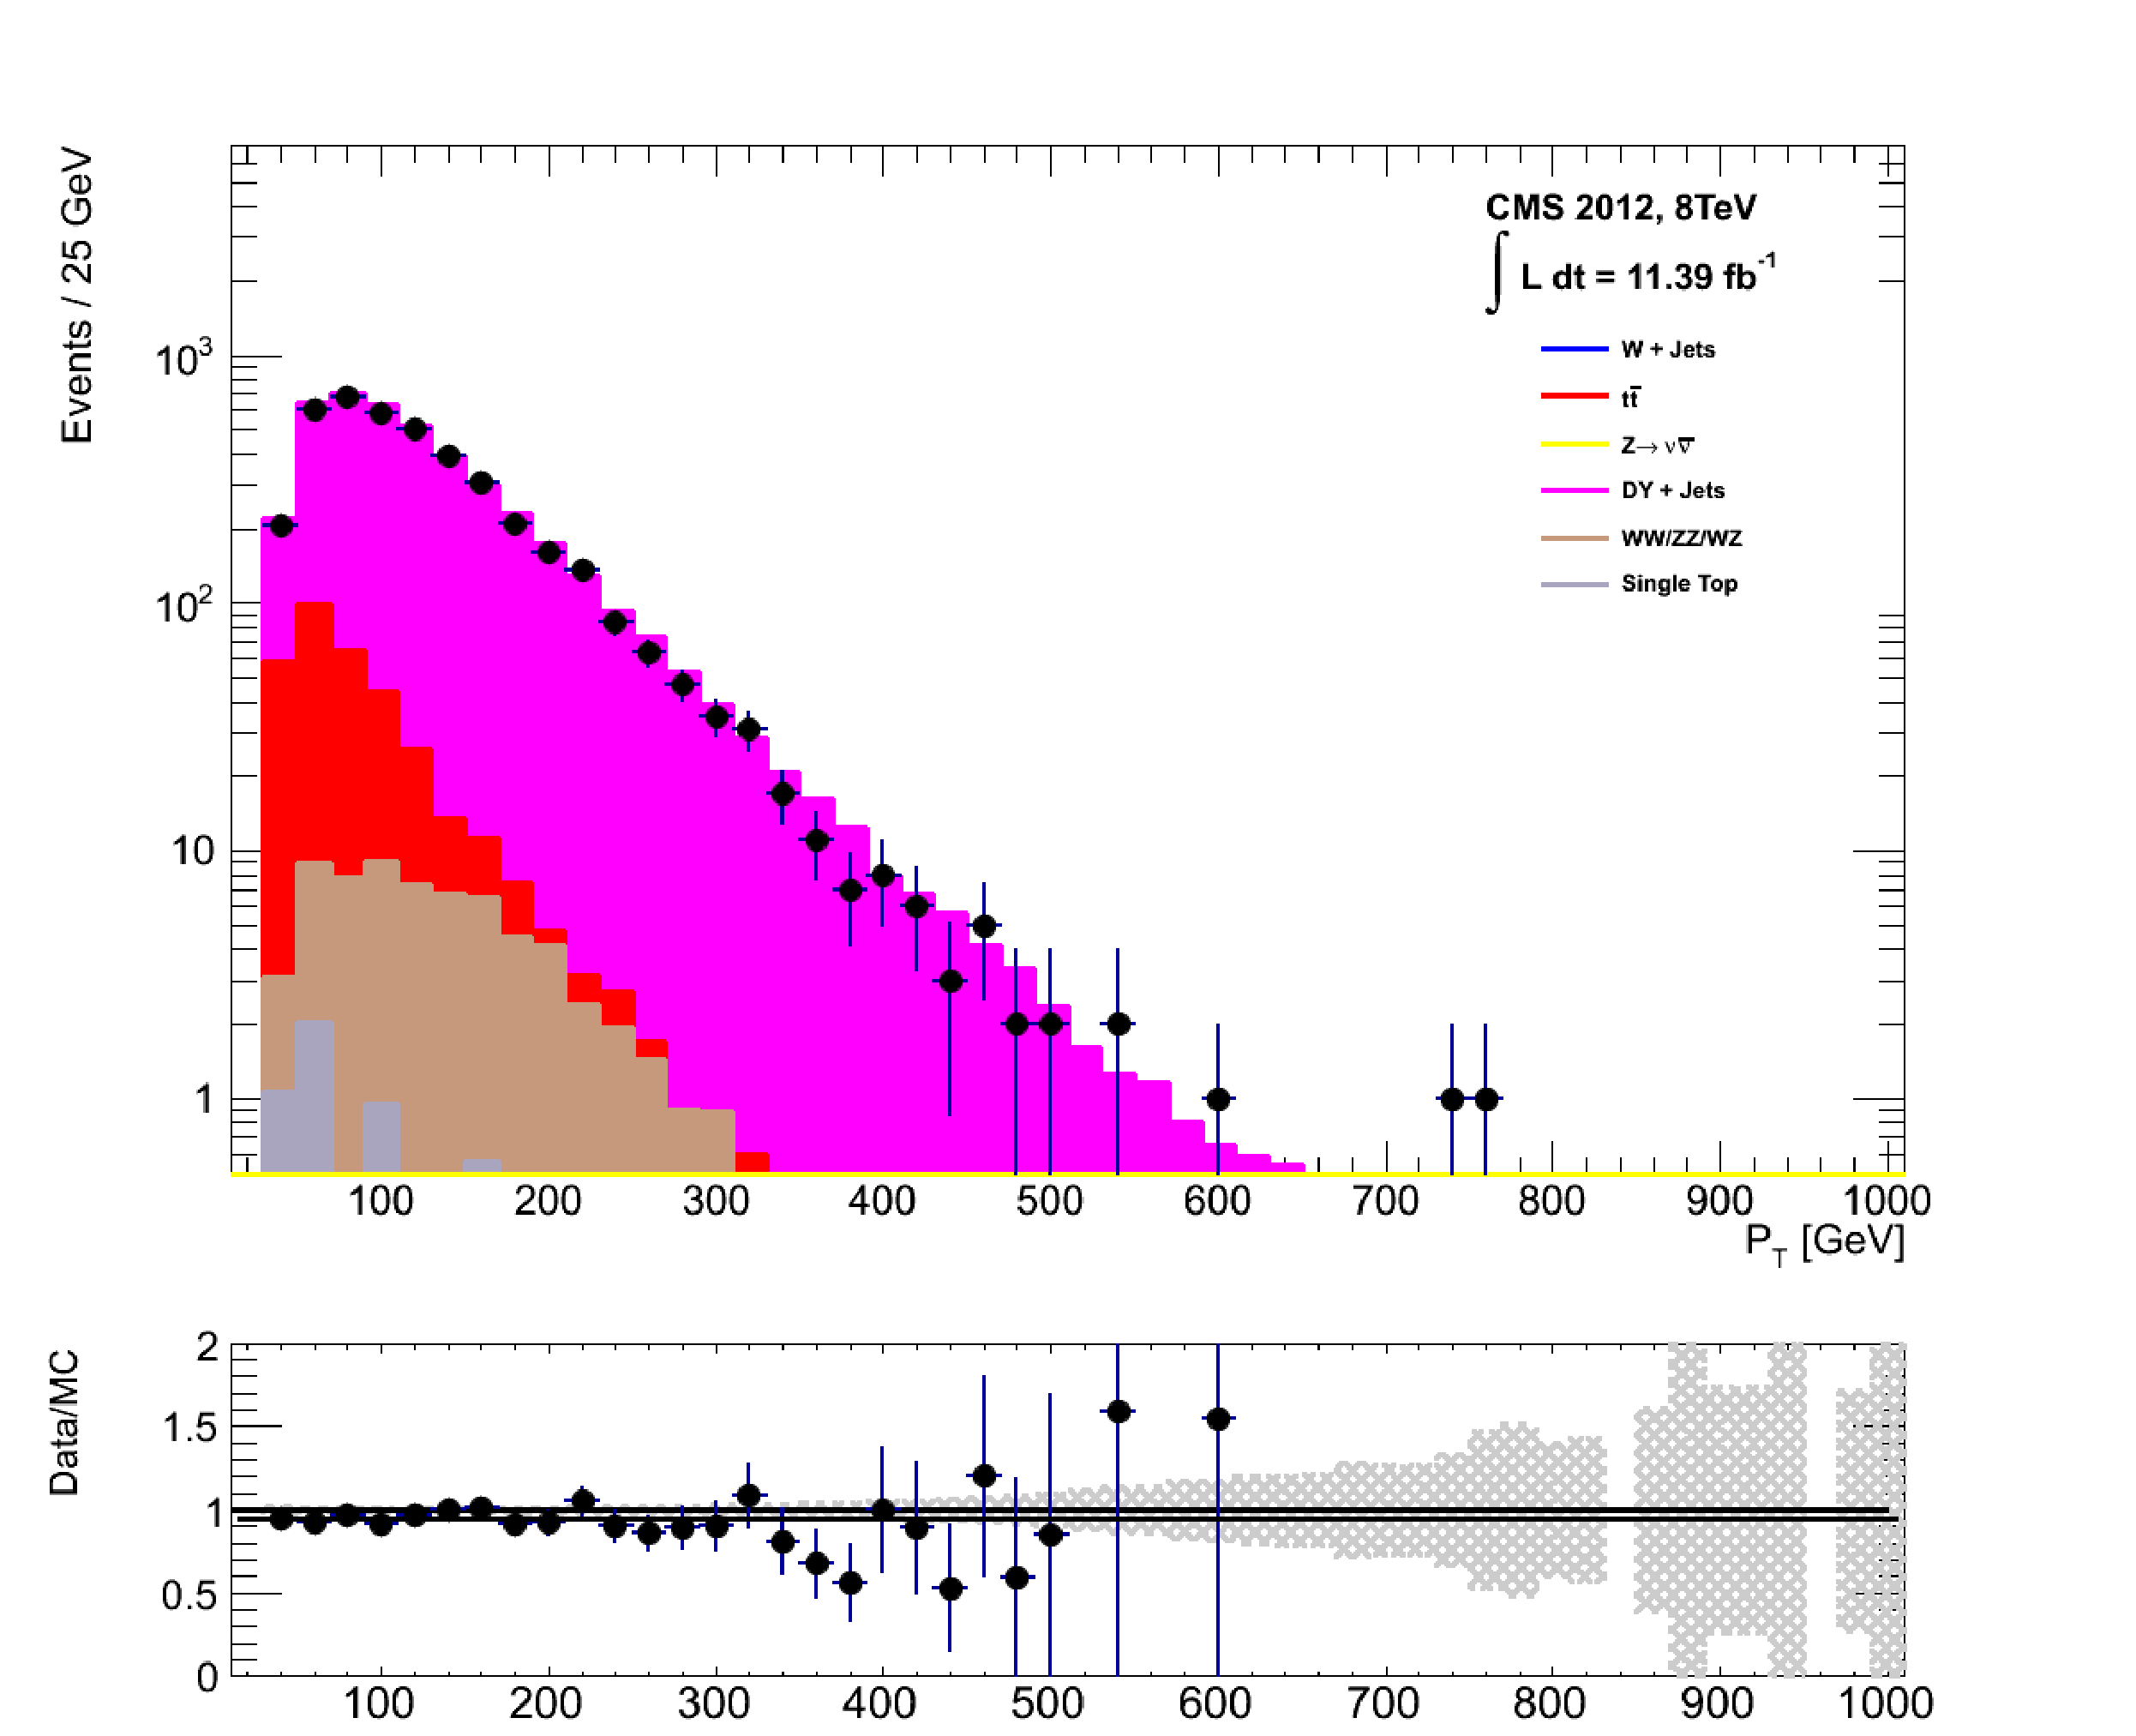
\includegraphics[width = 3.2in]{plots/dimuon_leadmu_datamc.pdf}
(a) Lead Muon \pt
\end{minipage}
\begin{minipage}{.48\textwidth}
\centering
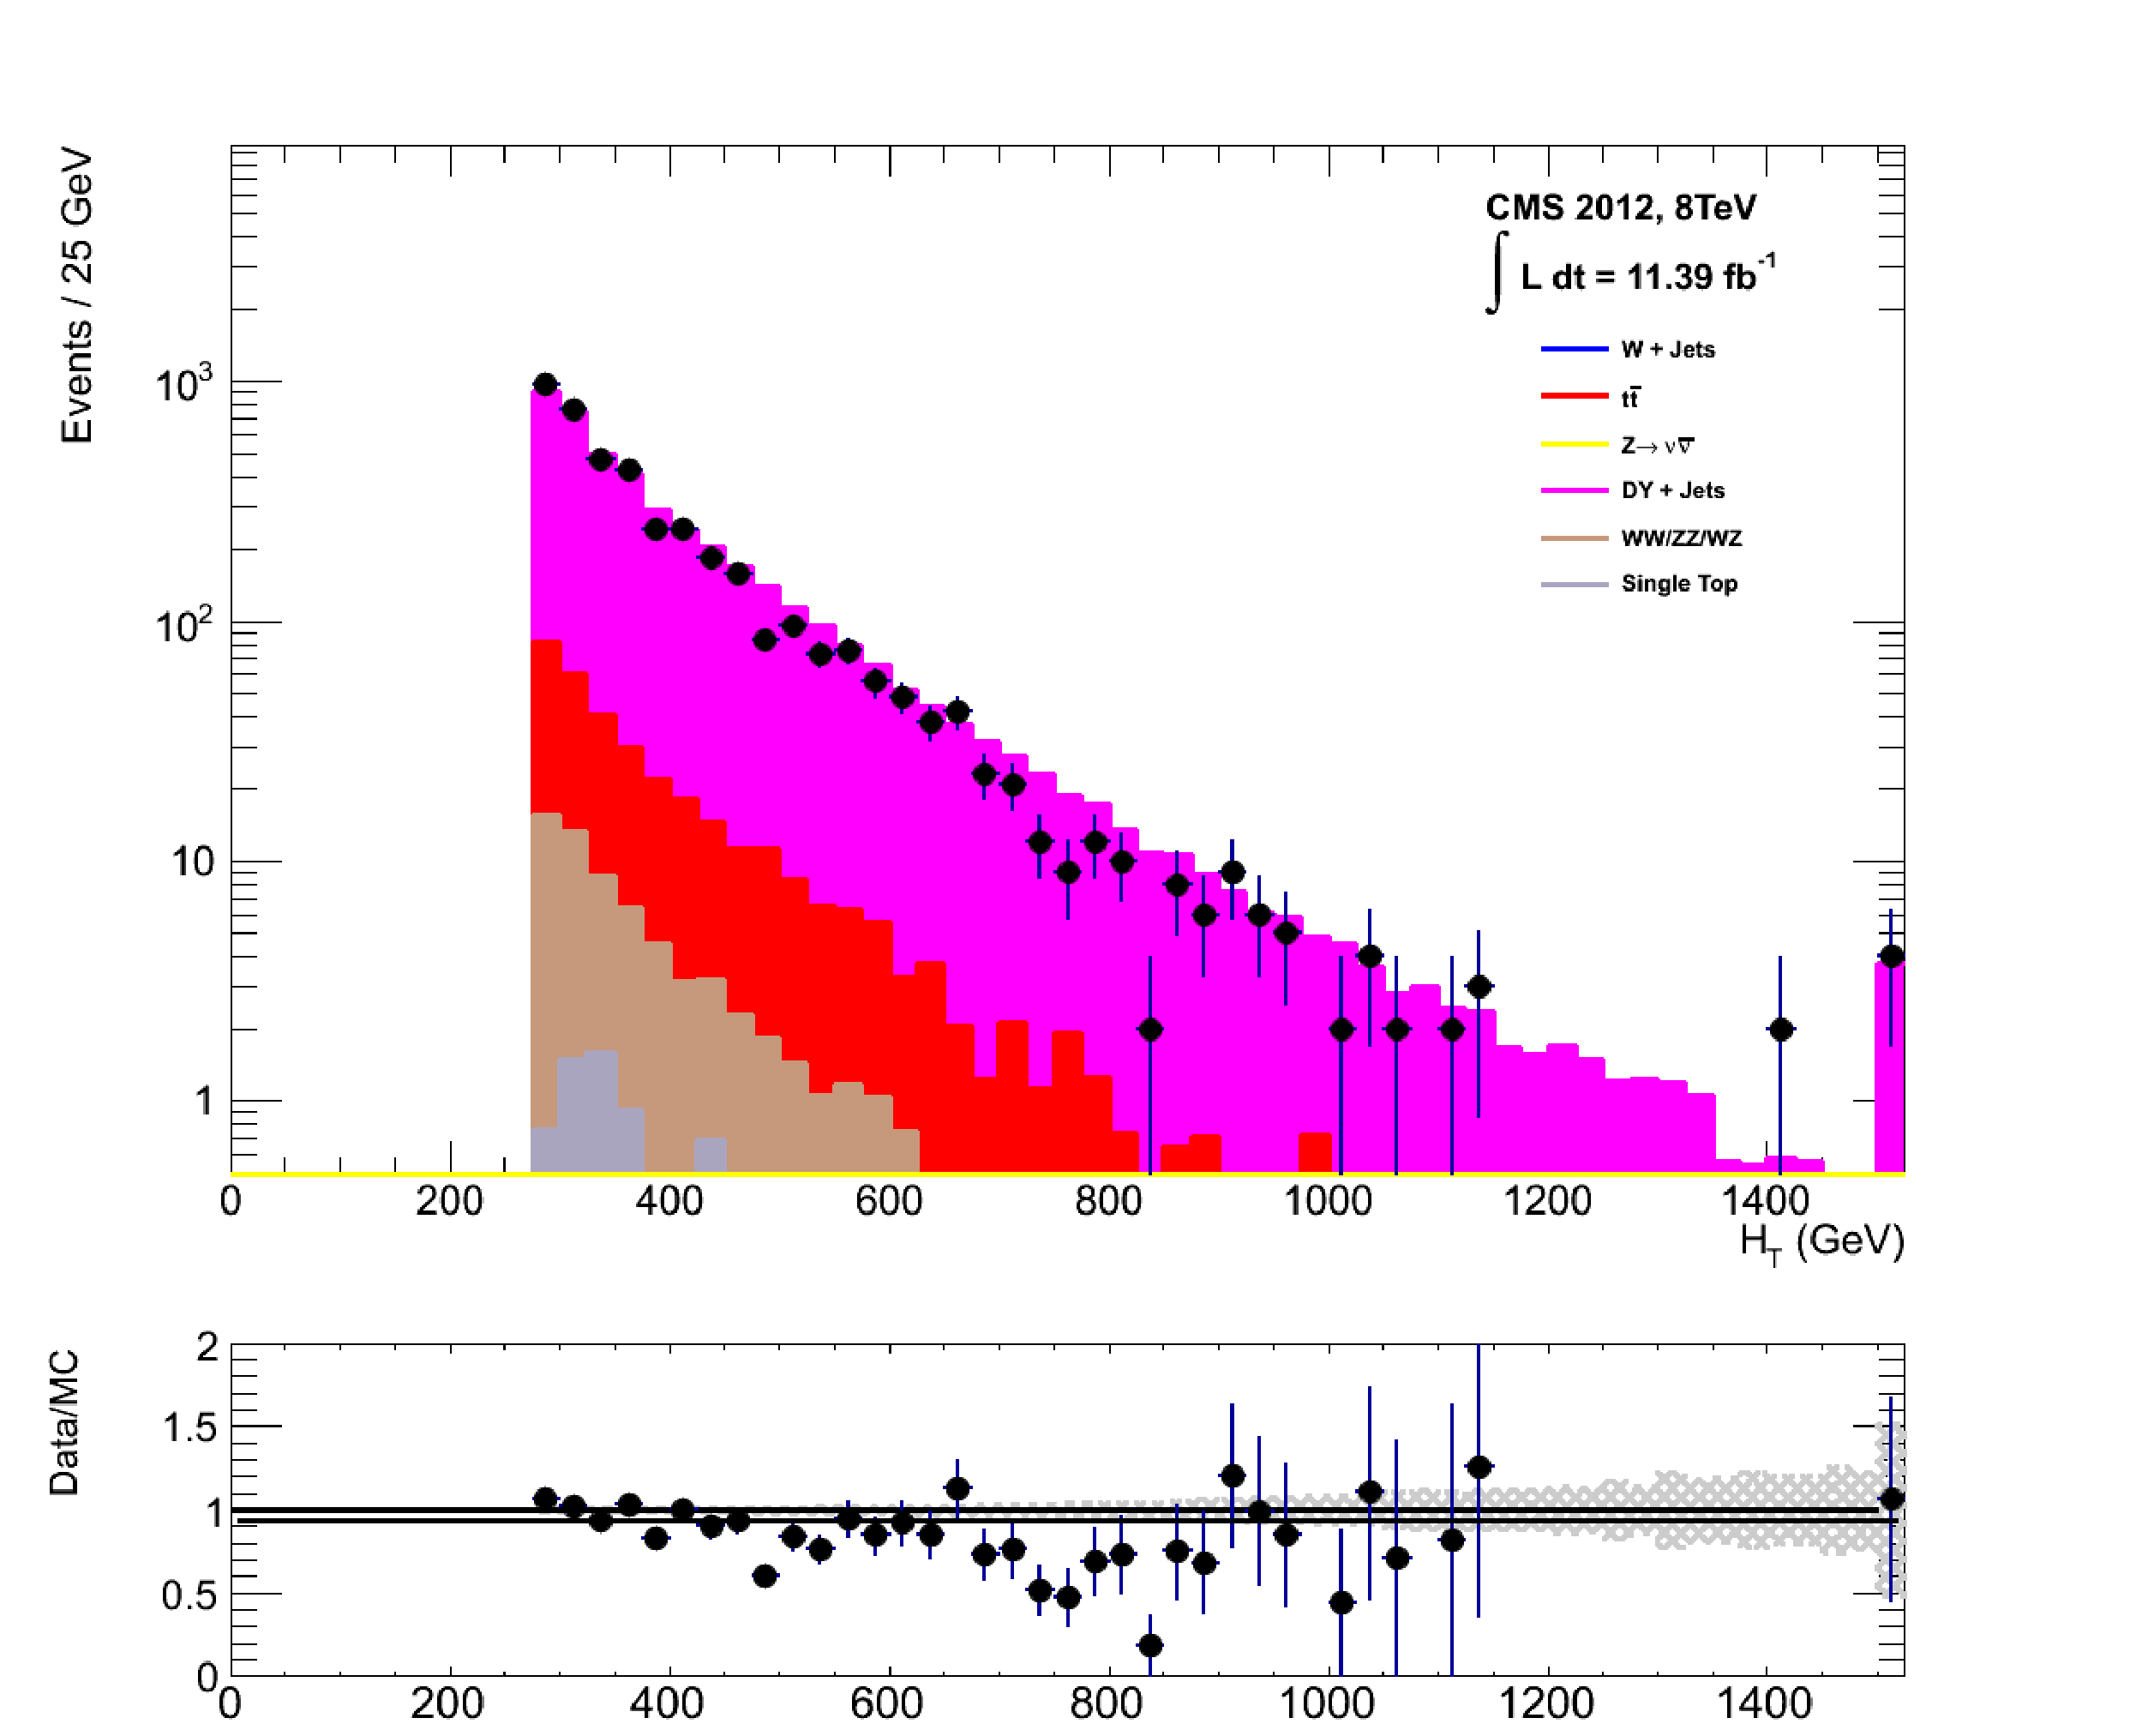
\includegraphics[width = 3.2in]{plots/dimuon_ht_datamc.pdf}
(b) \theht
\end{minipage}
\end{minipage}

\xspace

\begin{minipage}{\linewidth}
\centering
\begin{minipage}{.48\textwidth}
\centering
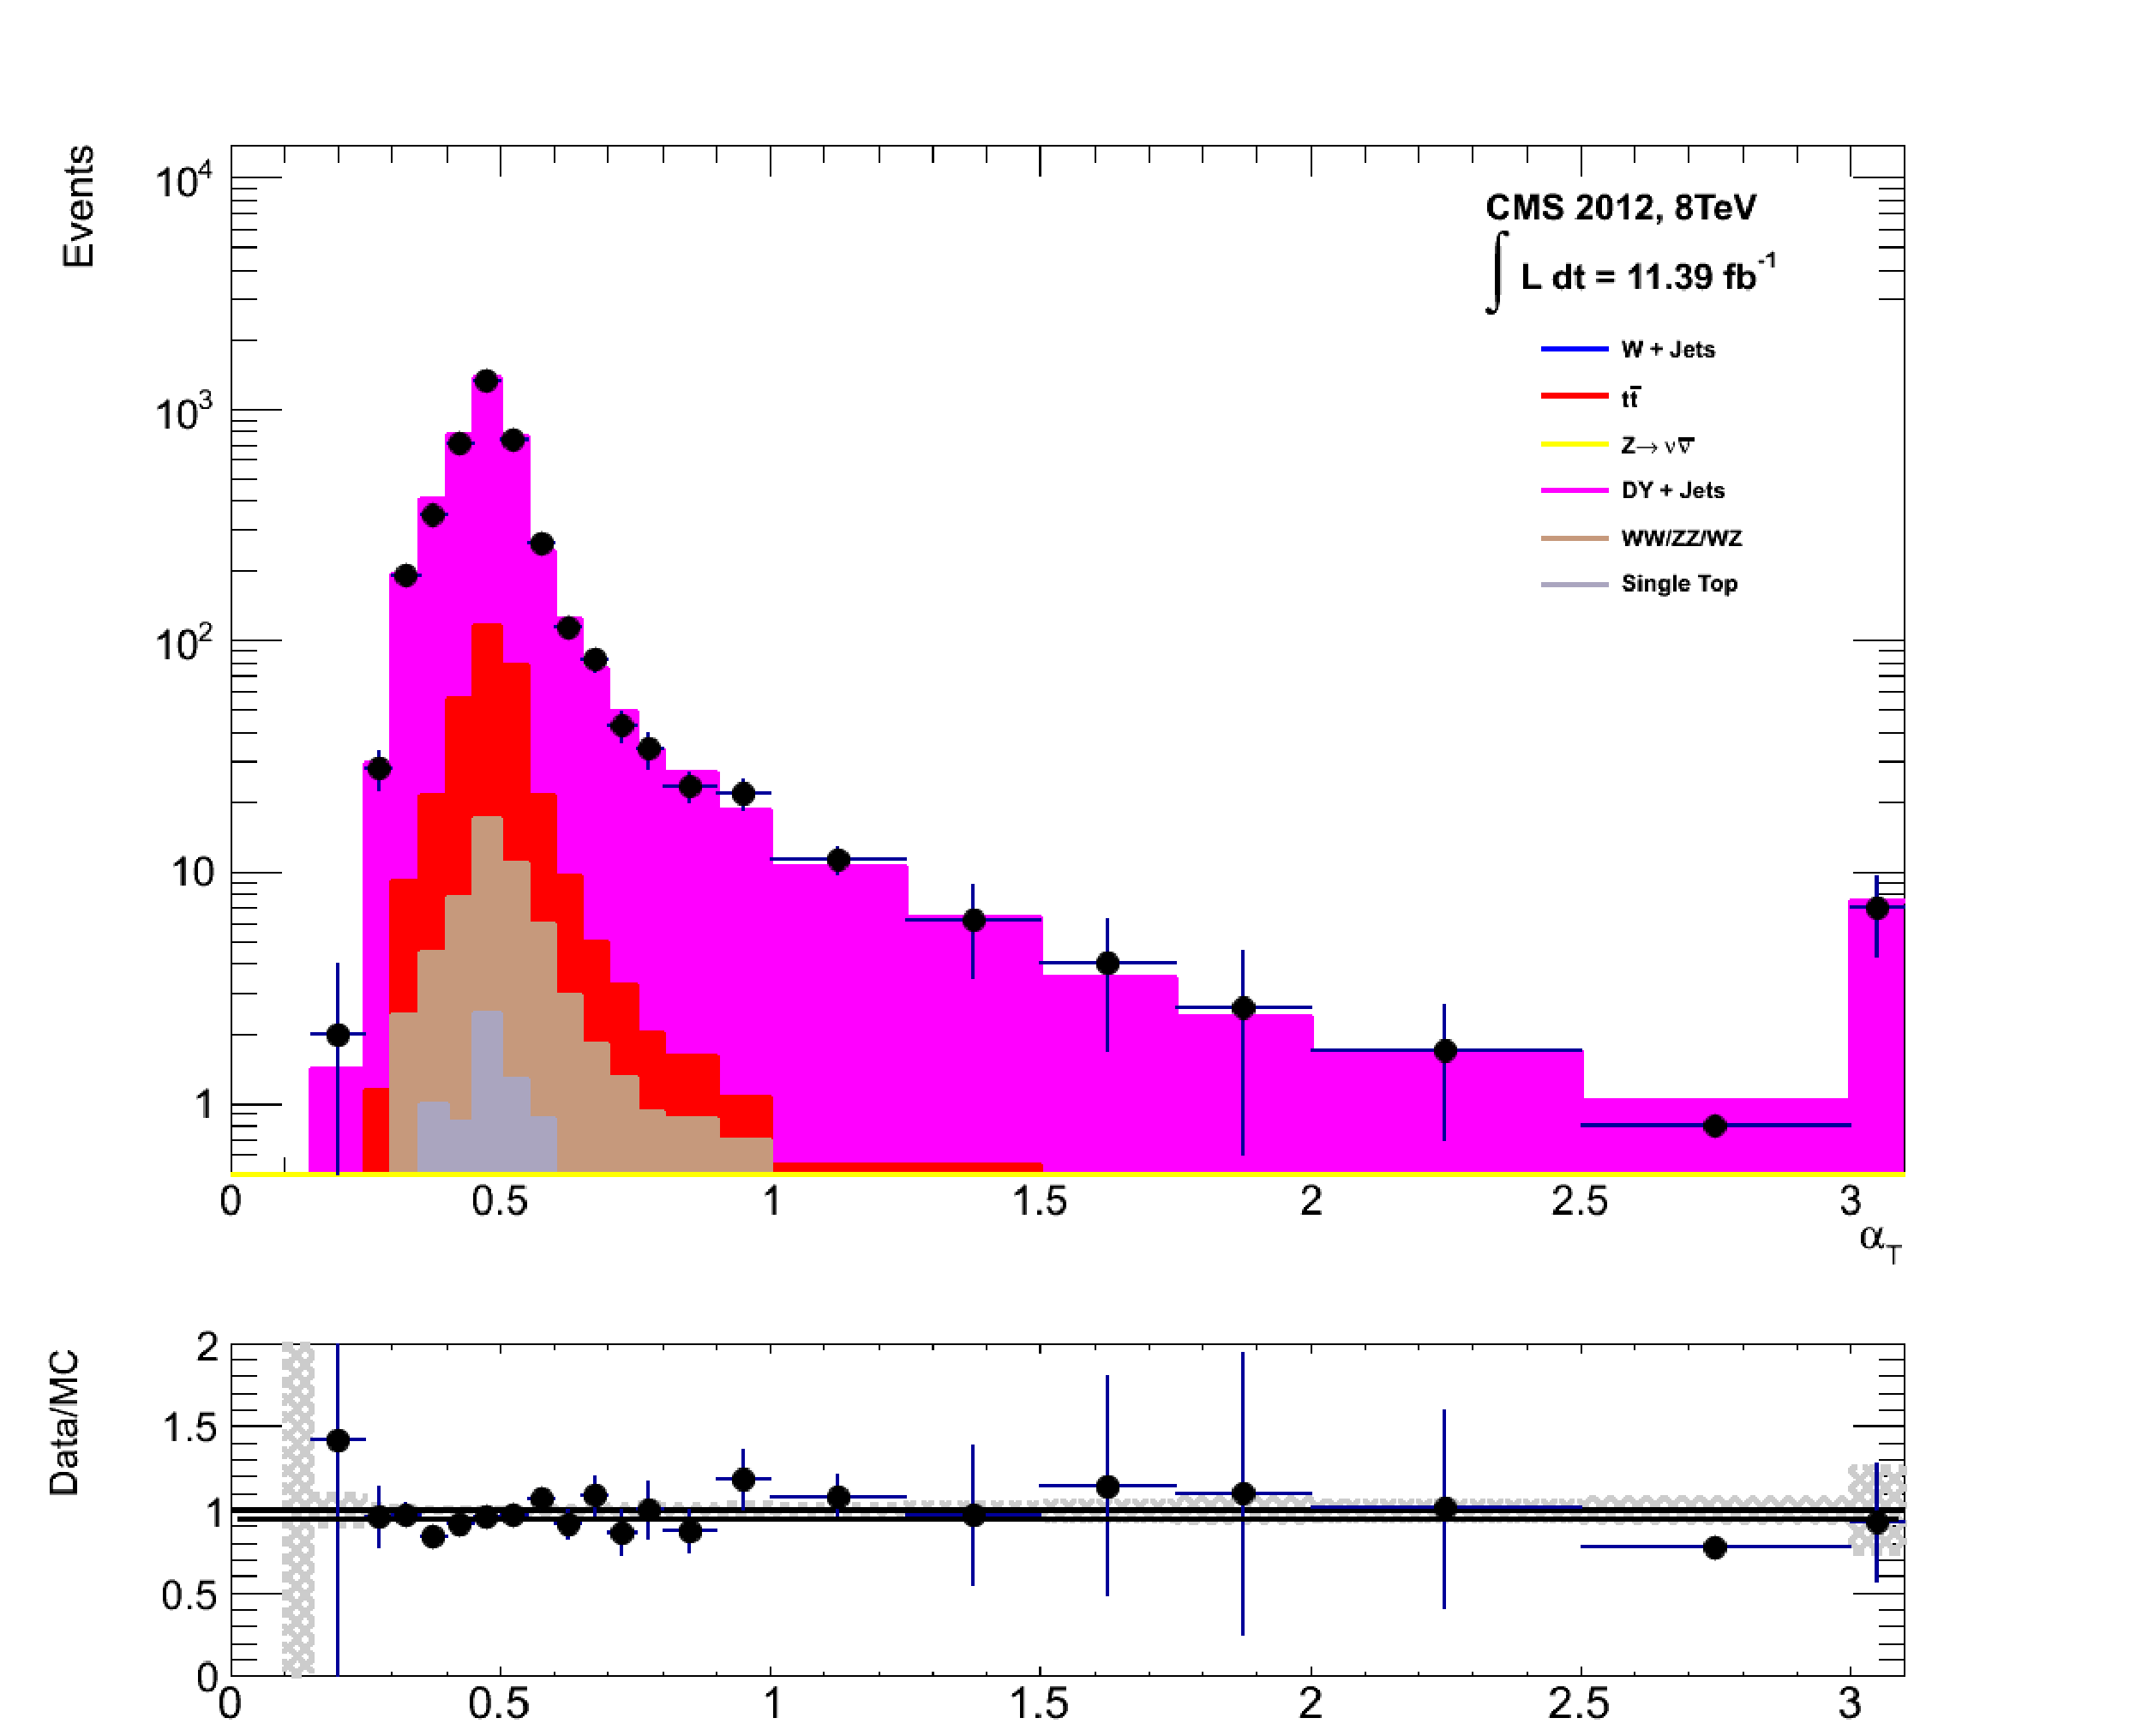
\includegraphics[width = 3.2in]{plots/dimuon_alphat_datamc.pdf}
$\text{(c}$) \alphat
\end{minipage}
\begin{minipage}{.48\textwidth}
\centering
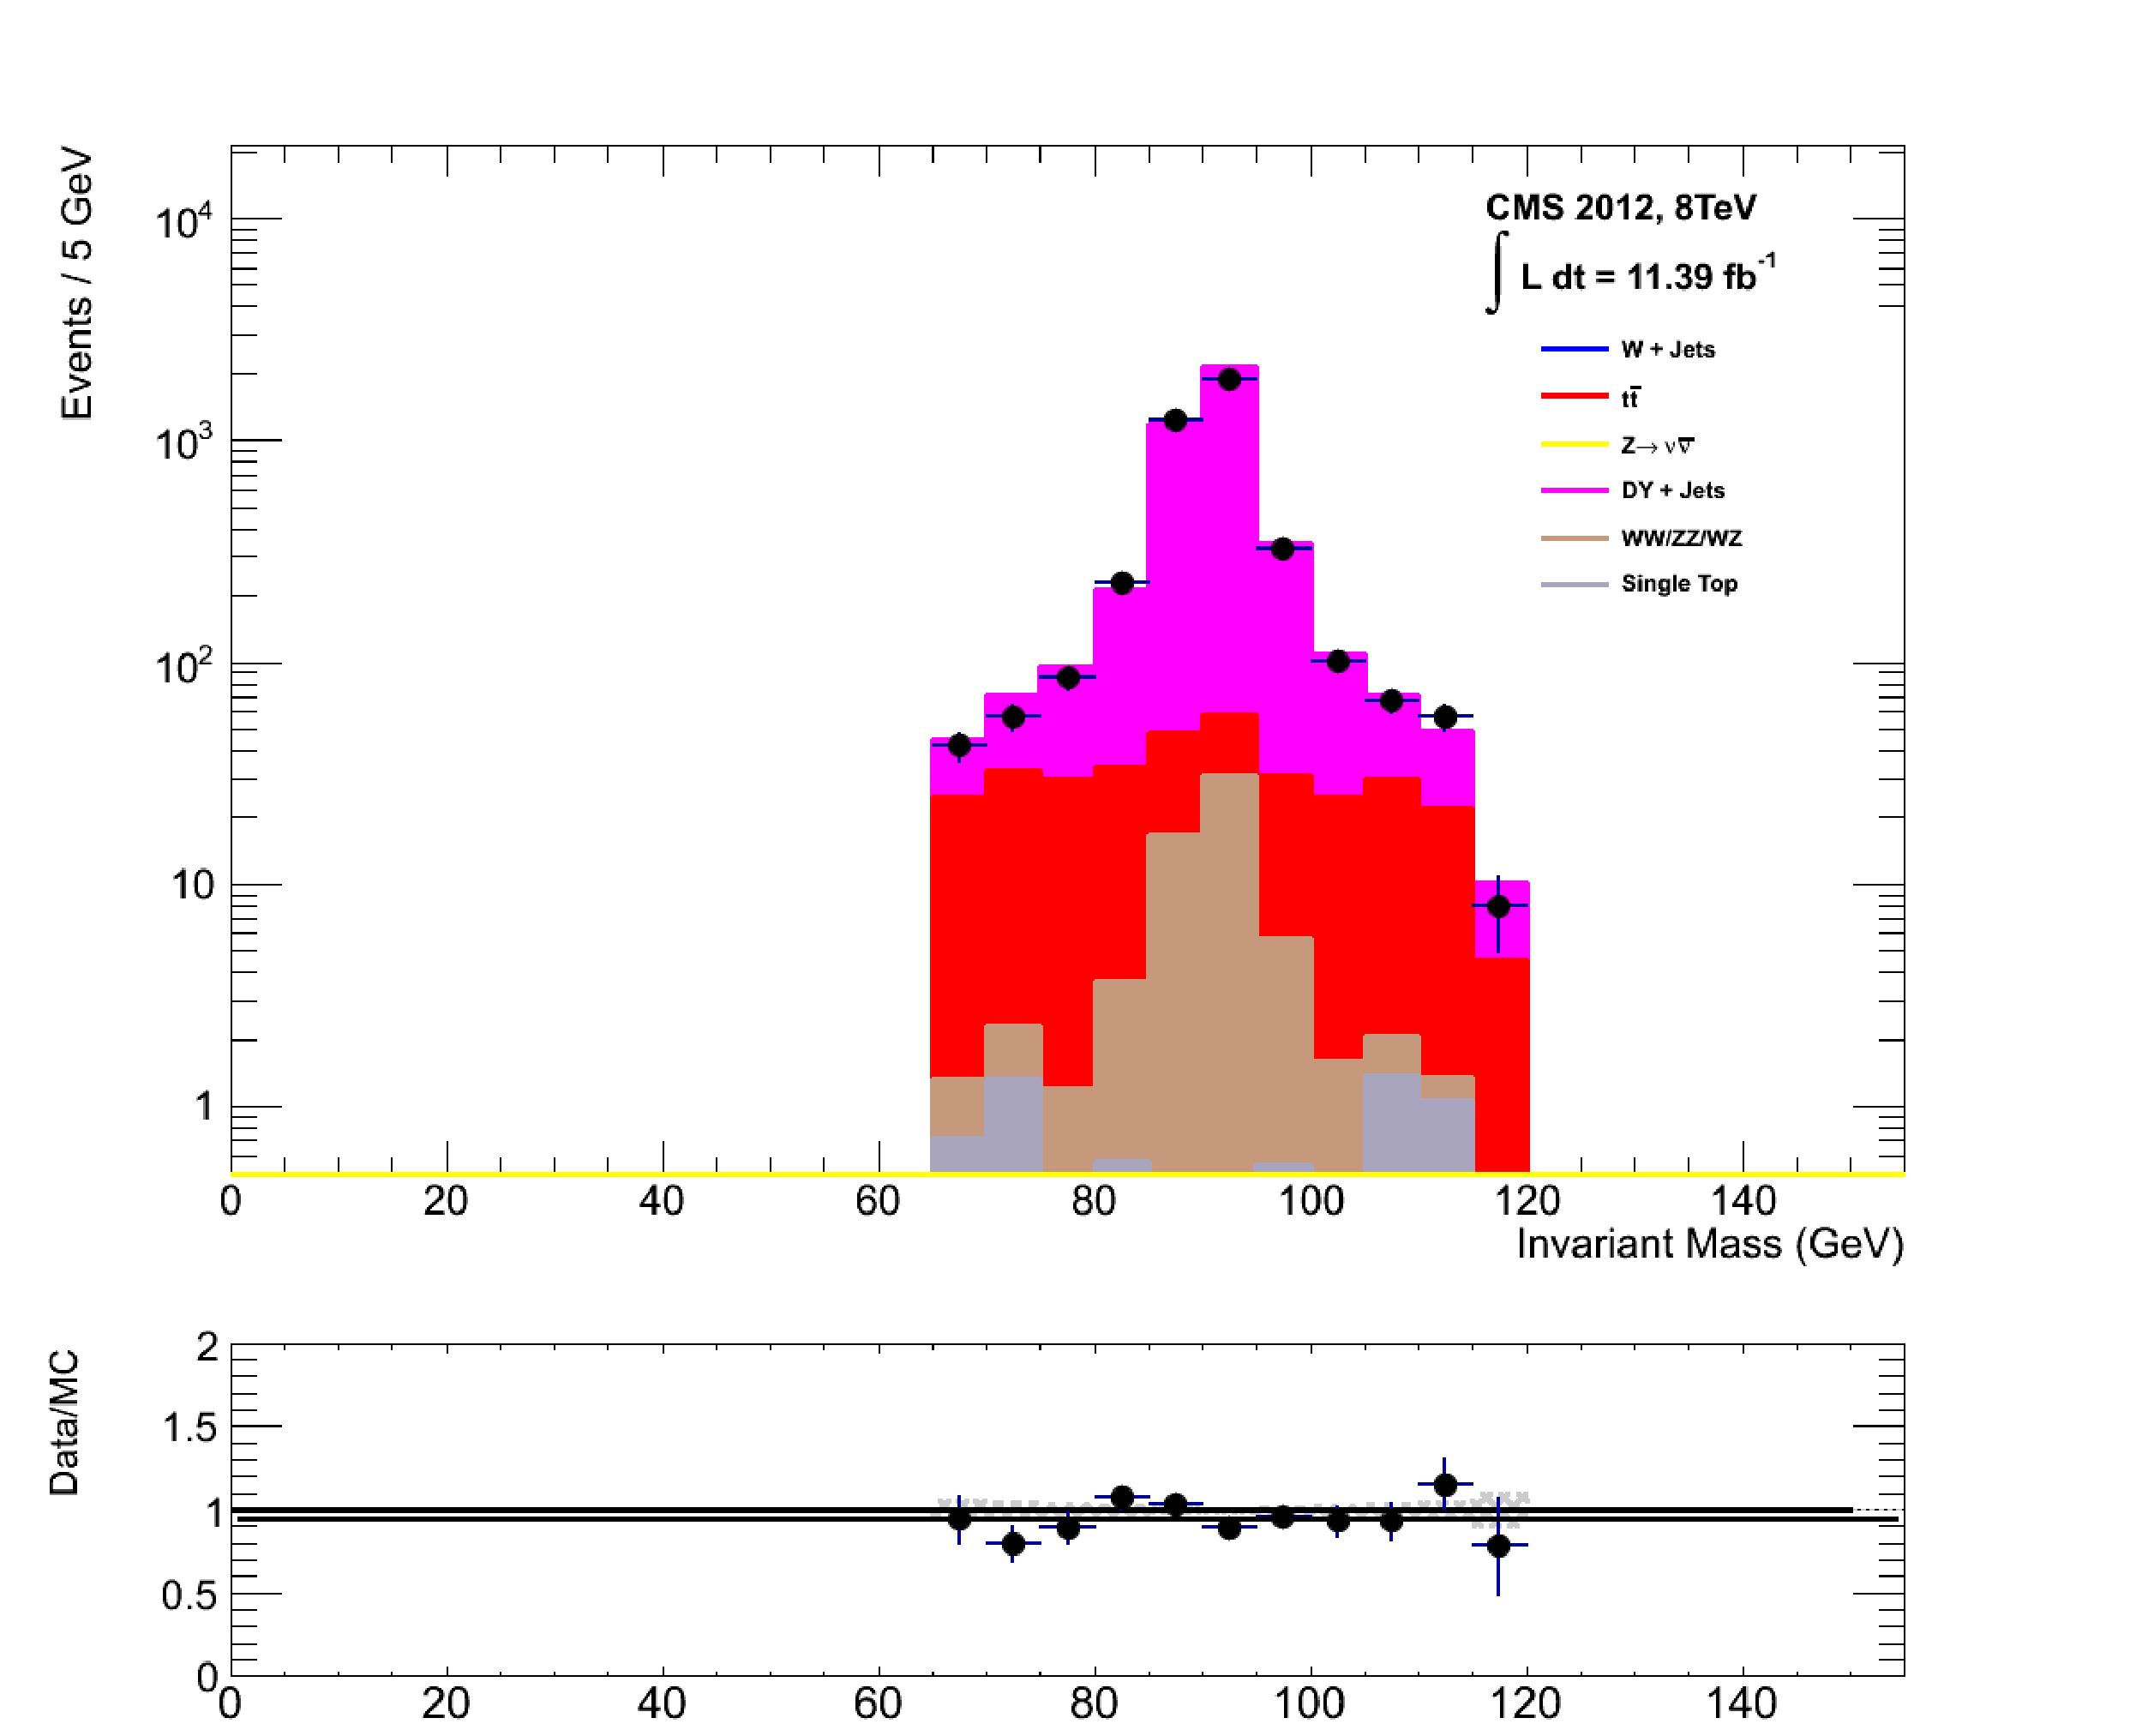
\includegraphics[width = 3.2in]{plots/dimuon_zmass_datamc.pdf}
(d) $\mu\mu$ invariant mass
\end{minipage}
\captionof{figure}[Data/MC comparisons of key variables for the \dimupjets selection.]{Data/MC comparisons of key variables for the \dimupjets selection,following the application of selection criteria and the requirements that \theht $>$ 275 \GeV. Bands represent the uncertainties due to the statistical size of the MC samples. No requirement is made upon the number of b-tagged jets or jet multiplicity in these distributions.}\label{fig:dimuonmcplots}
\end{minipage}


\item[] \textbf{The \gpjets control sample}

The \zinv + jets background is also estimated from a \gpjets control sample, which possesses a larger cross section and kinematic properties similar to those of \zmumu events where the photon is ignored \cite{PhysRevD.84.114002}\cite{CMS-PAS-SUS-08-002}. The photon is ignored for the purpose of the calculation of event level variables, and identical selection cuts to the hadronic signal region are applied. 

\begin{itemize}
\item Exactly one photon is selected, satisfying identification criteria as detailed in Table \ref{tab:photonidtable}, with a minimum \pt $> $165 \GeV to satisfy trigger thresholds and \abeta $<$ 1.45 to ensure the photon remains in the barrel of the detector.
\item A selection criteria of $\Delta R(\gamma,jet) <$ 1.0, between the photon and all jets is applied to ensure the acceptance of only well isolated \gpjets events. 
\item Given that the photon is ignored, this control sample can only be applied in the \theht region $>$ 375 \GeV, due to the trigger thresholds on the minimum \pt of the photon, and the \mht requirement of an \alphat $>$ 0.55 cut from Equation (\ref{eq:alphatmht}). 
\end{itemize}


\begin{minipage}{\linewidth}
\centering
\begin{minipage}{.48\textwidth}
\centering
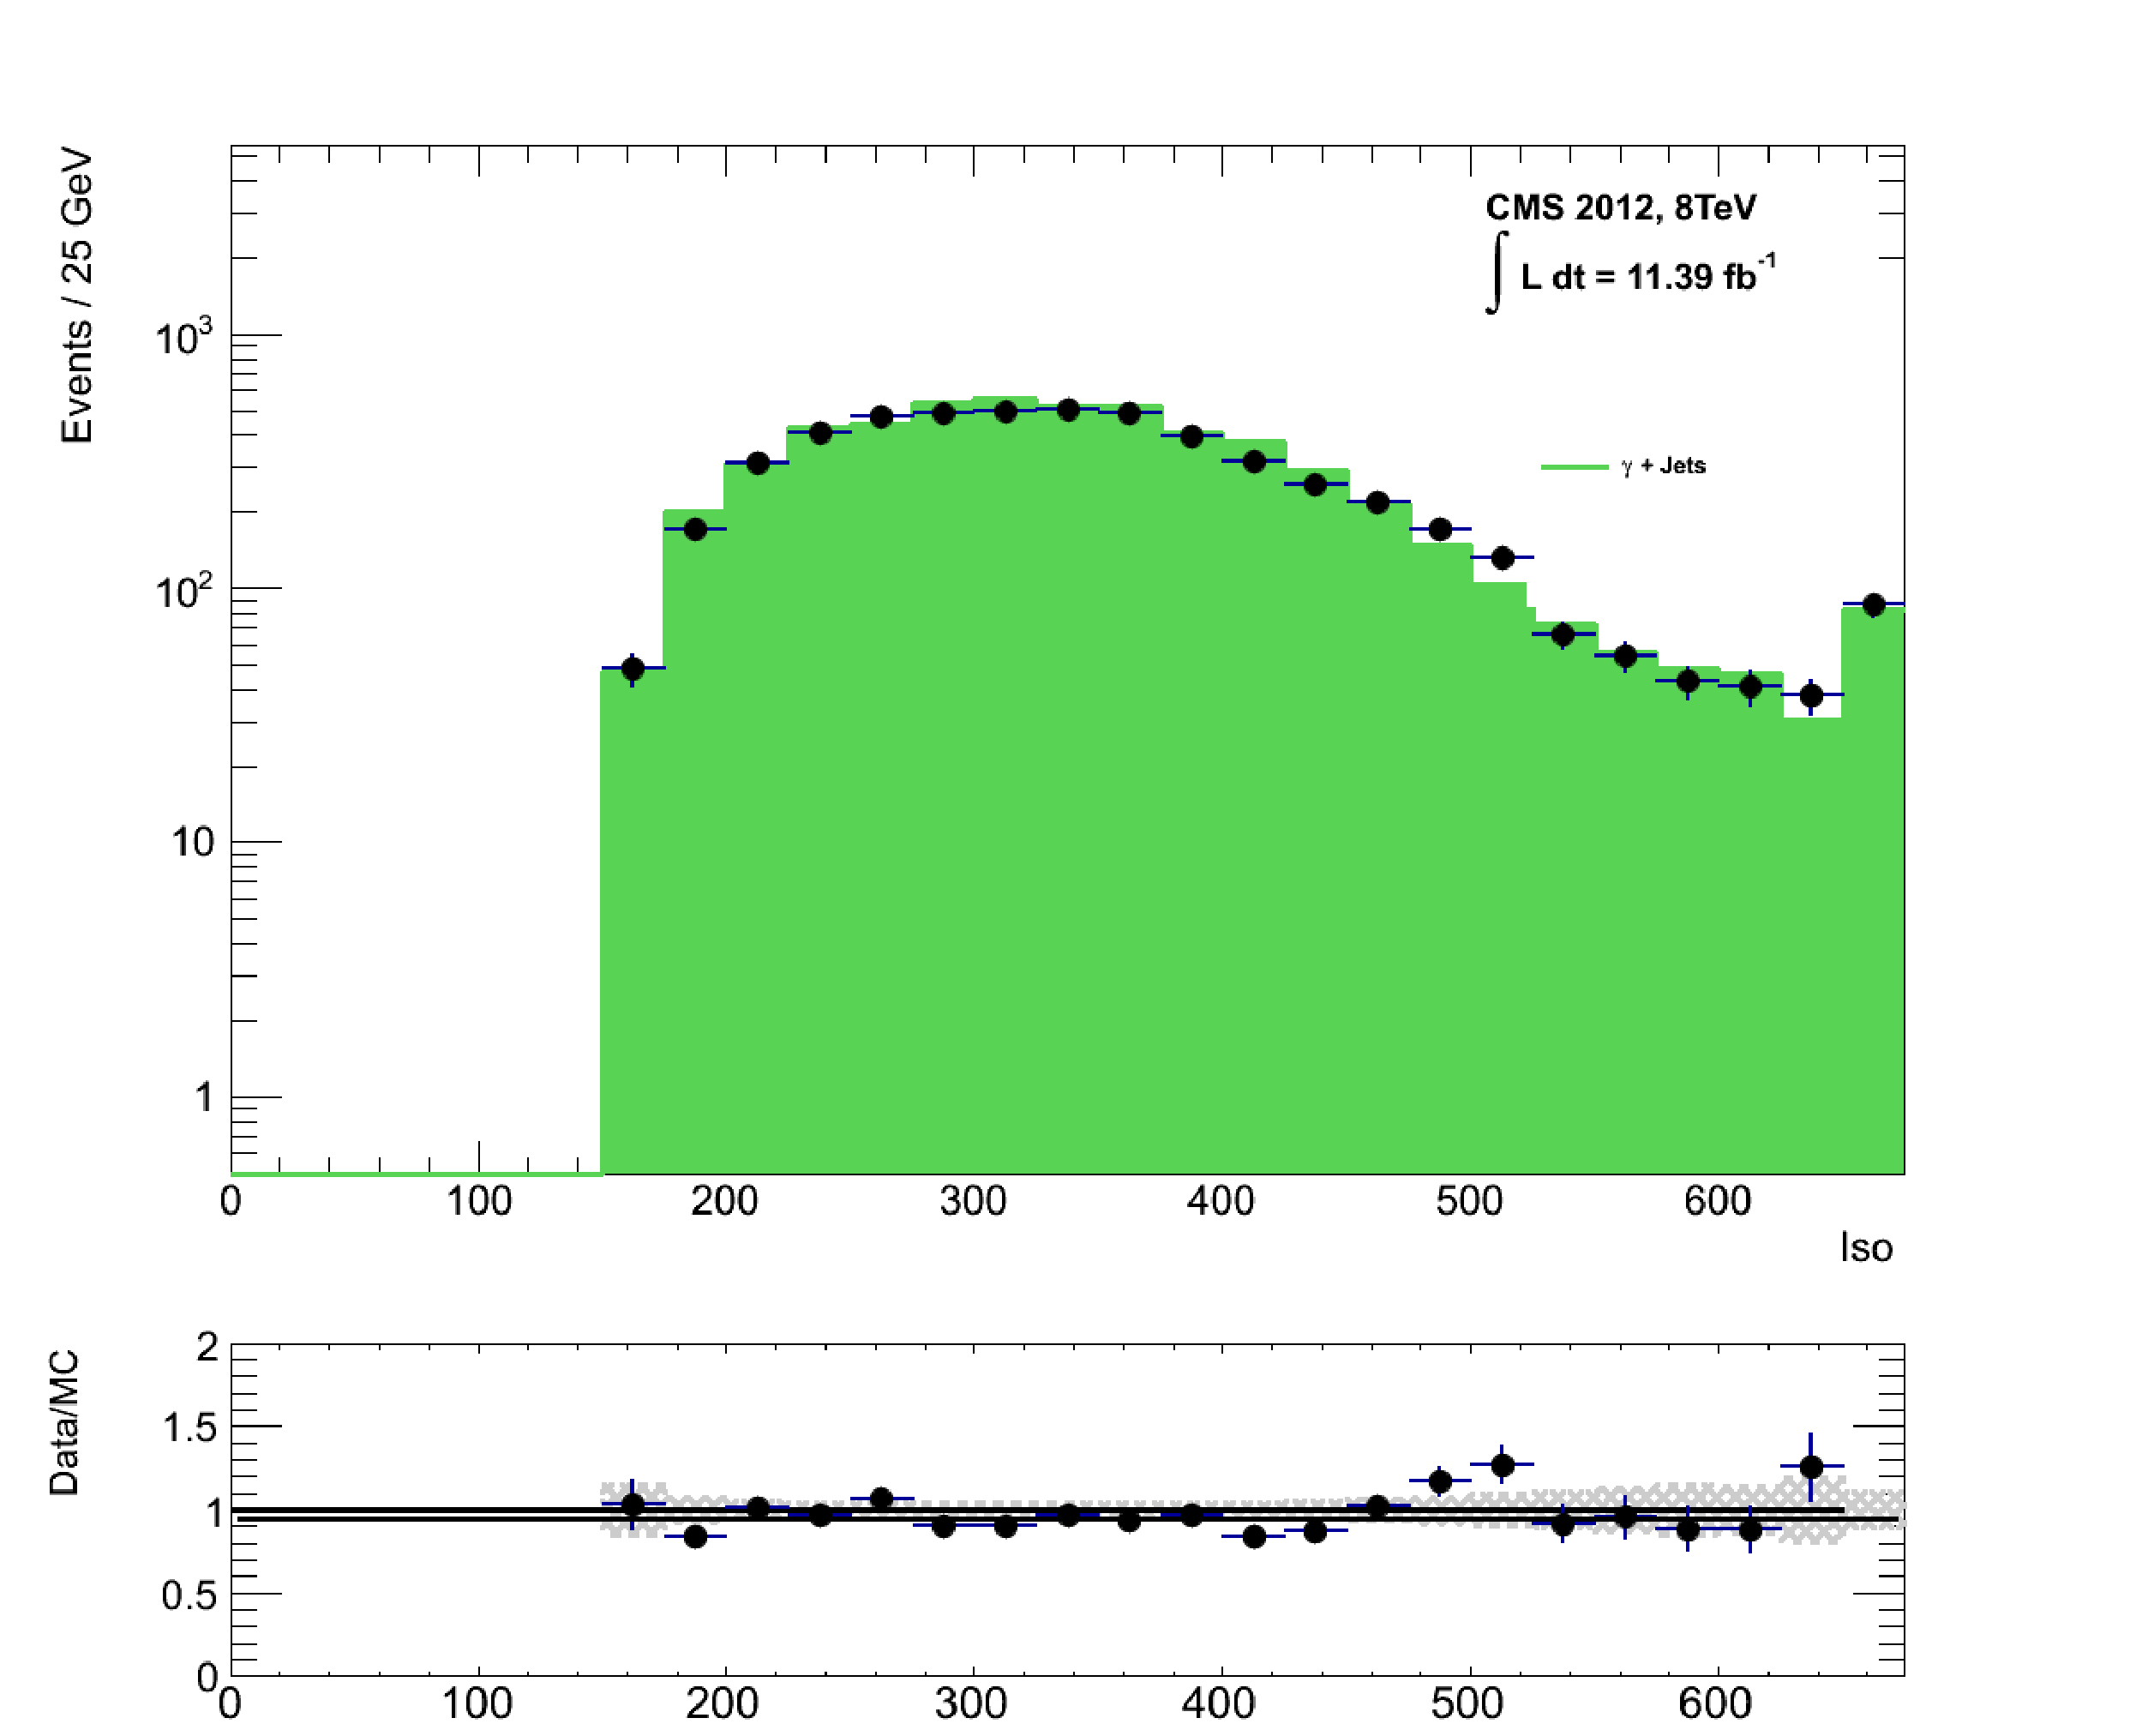
\includegraphics[width = 3.2in]{plots/photon_leadphoton_datamc.pdf}
(a) Lead Photon \pt
\end{minipage}
\begin{minipage}{.48\textwidth}
\centering
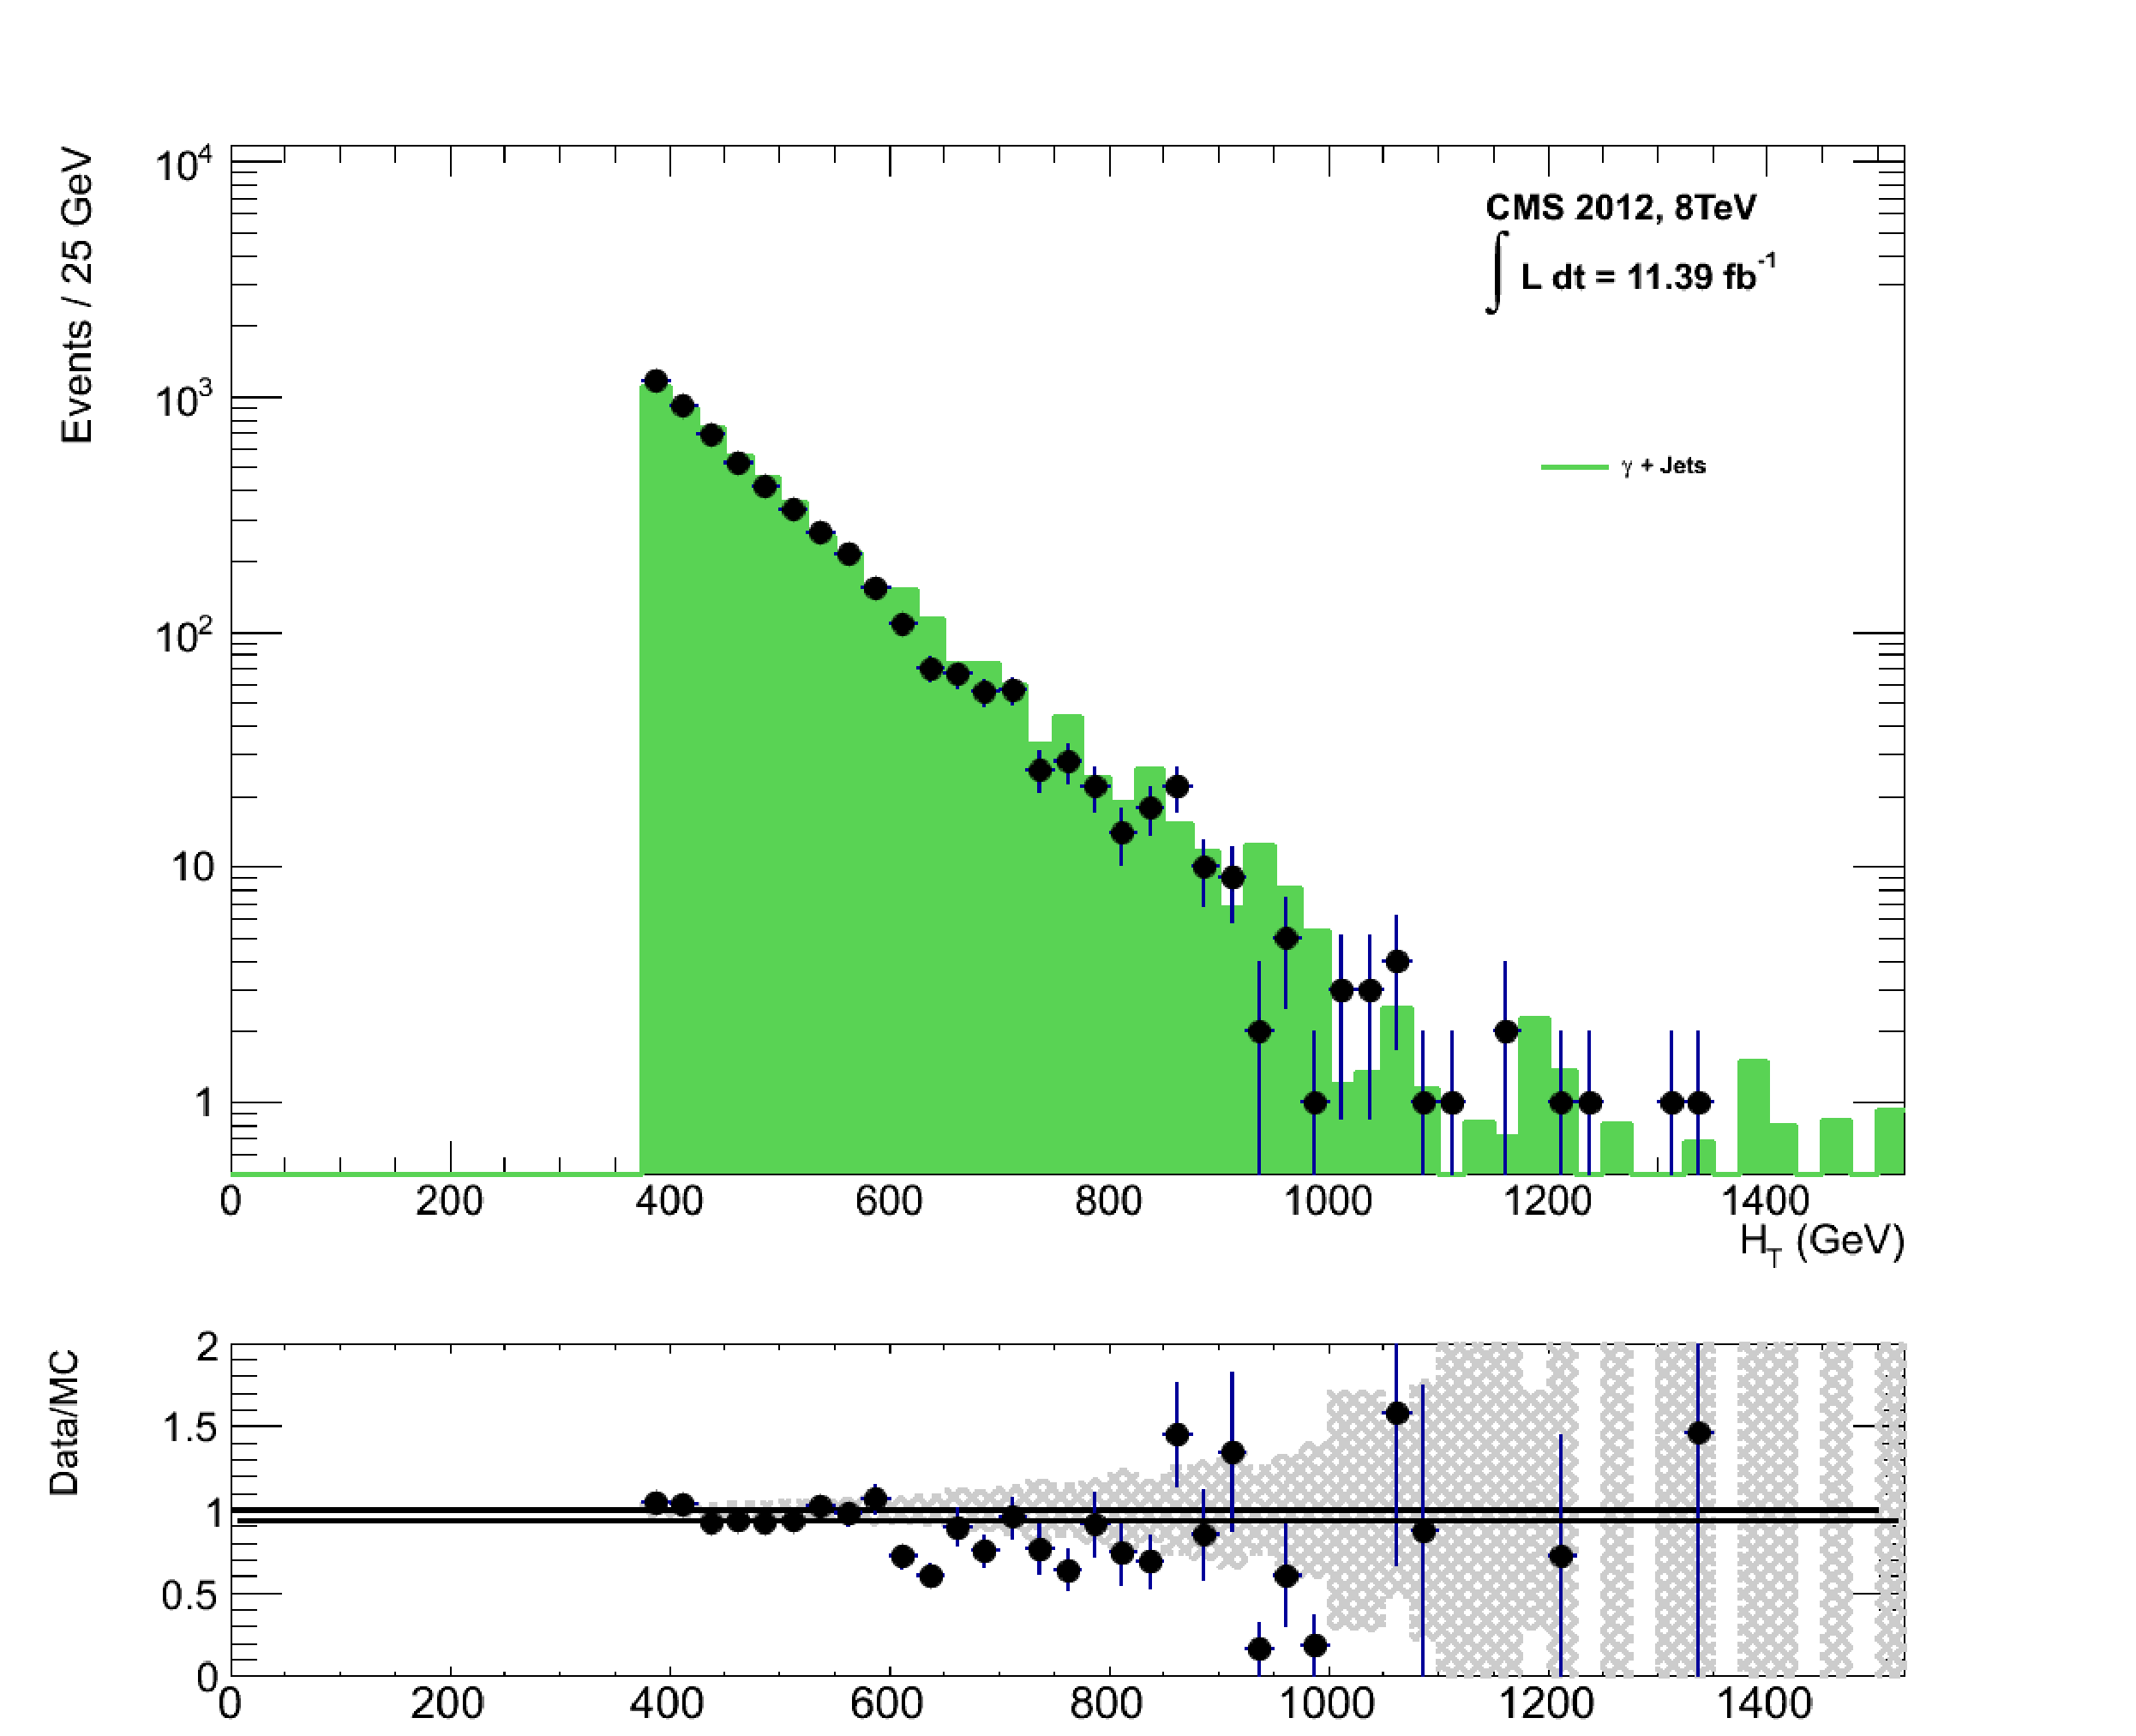
\includegraphics[width = 3.2in]{plots/photon_ht_datamc.pdf}
(b) \theht
\end{minipage}
\begin{minipage}{.48\textwidth}
\centering
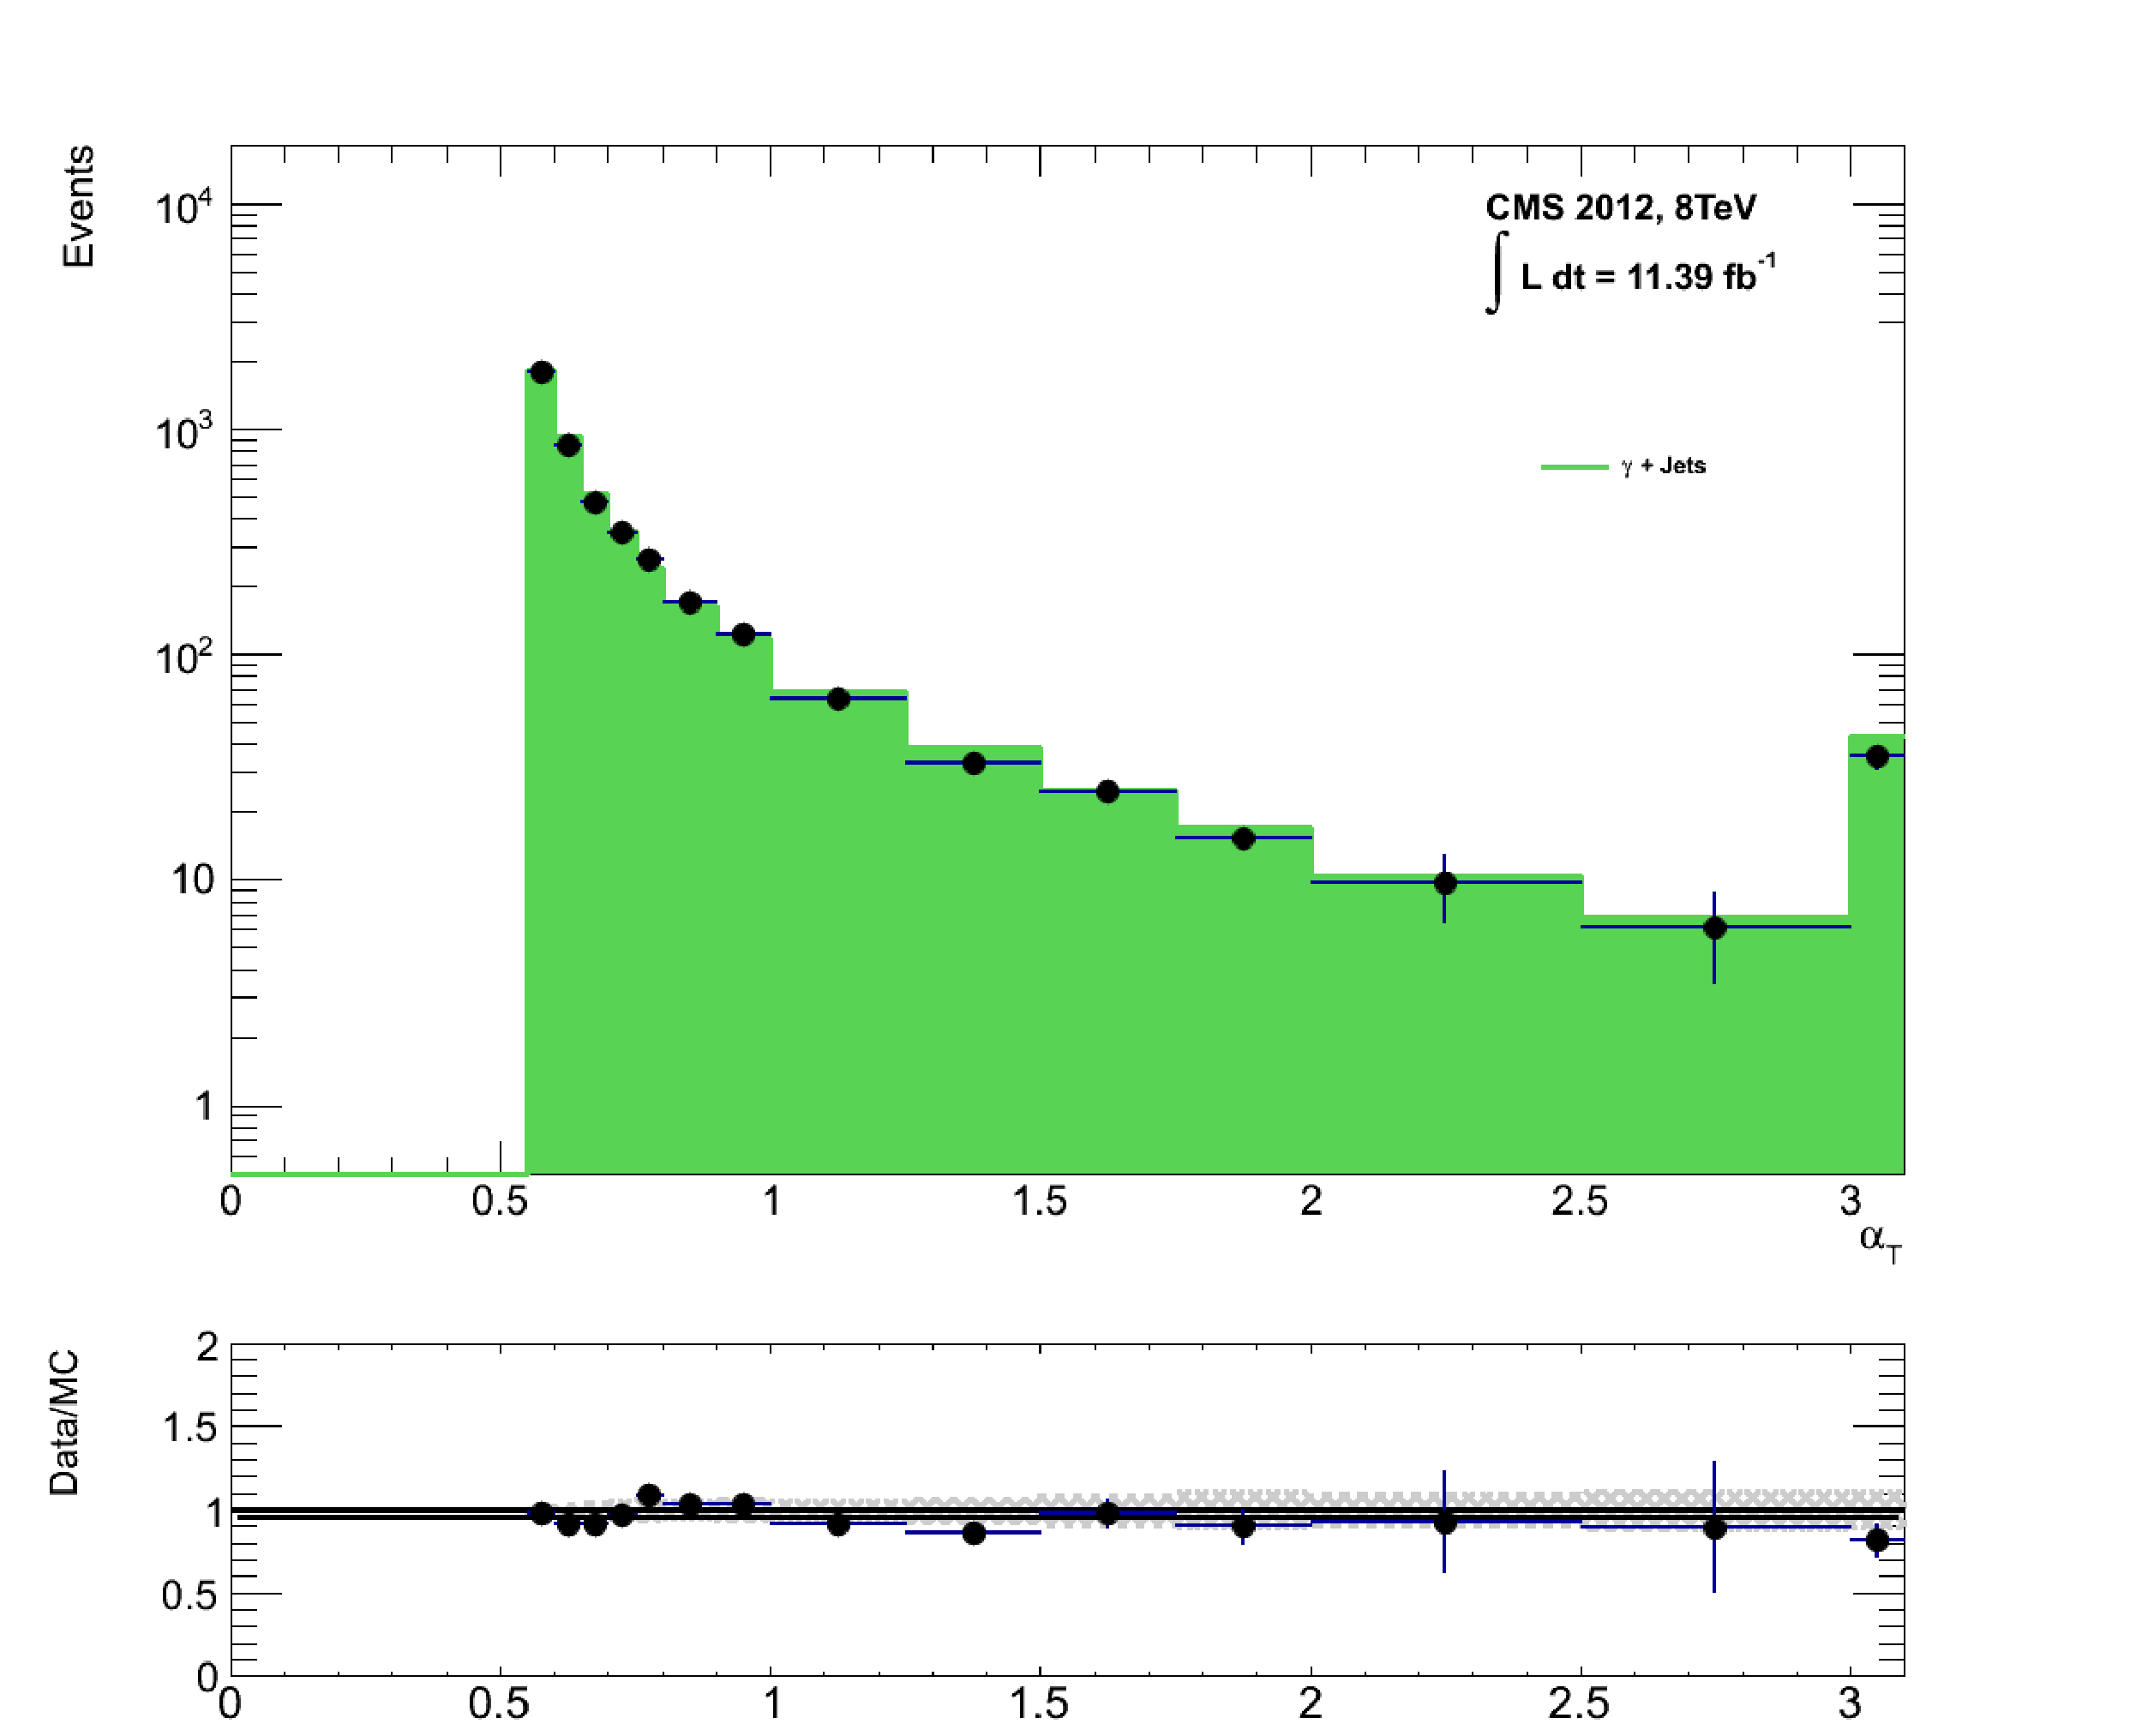
\includegraphics[width = 3.2in]{plots/photon_alphat_datamc.pdf}
$\text{(c}$) \alphat
\end{minipage}
\begin{minipage}{.48\textwidth}
\centering
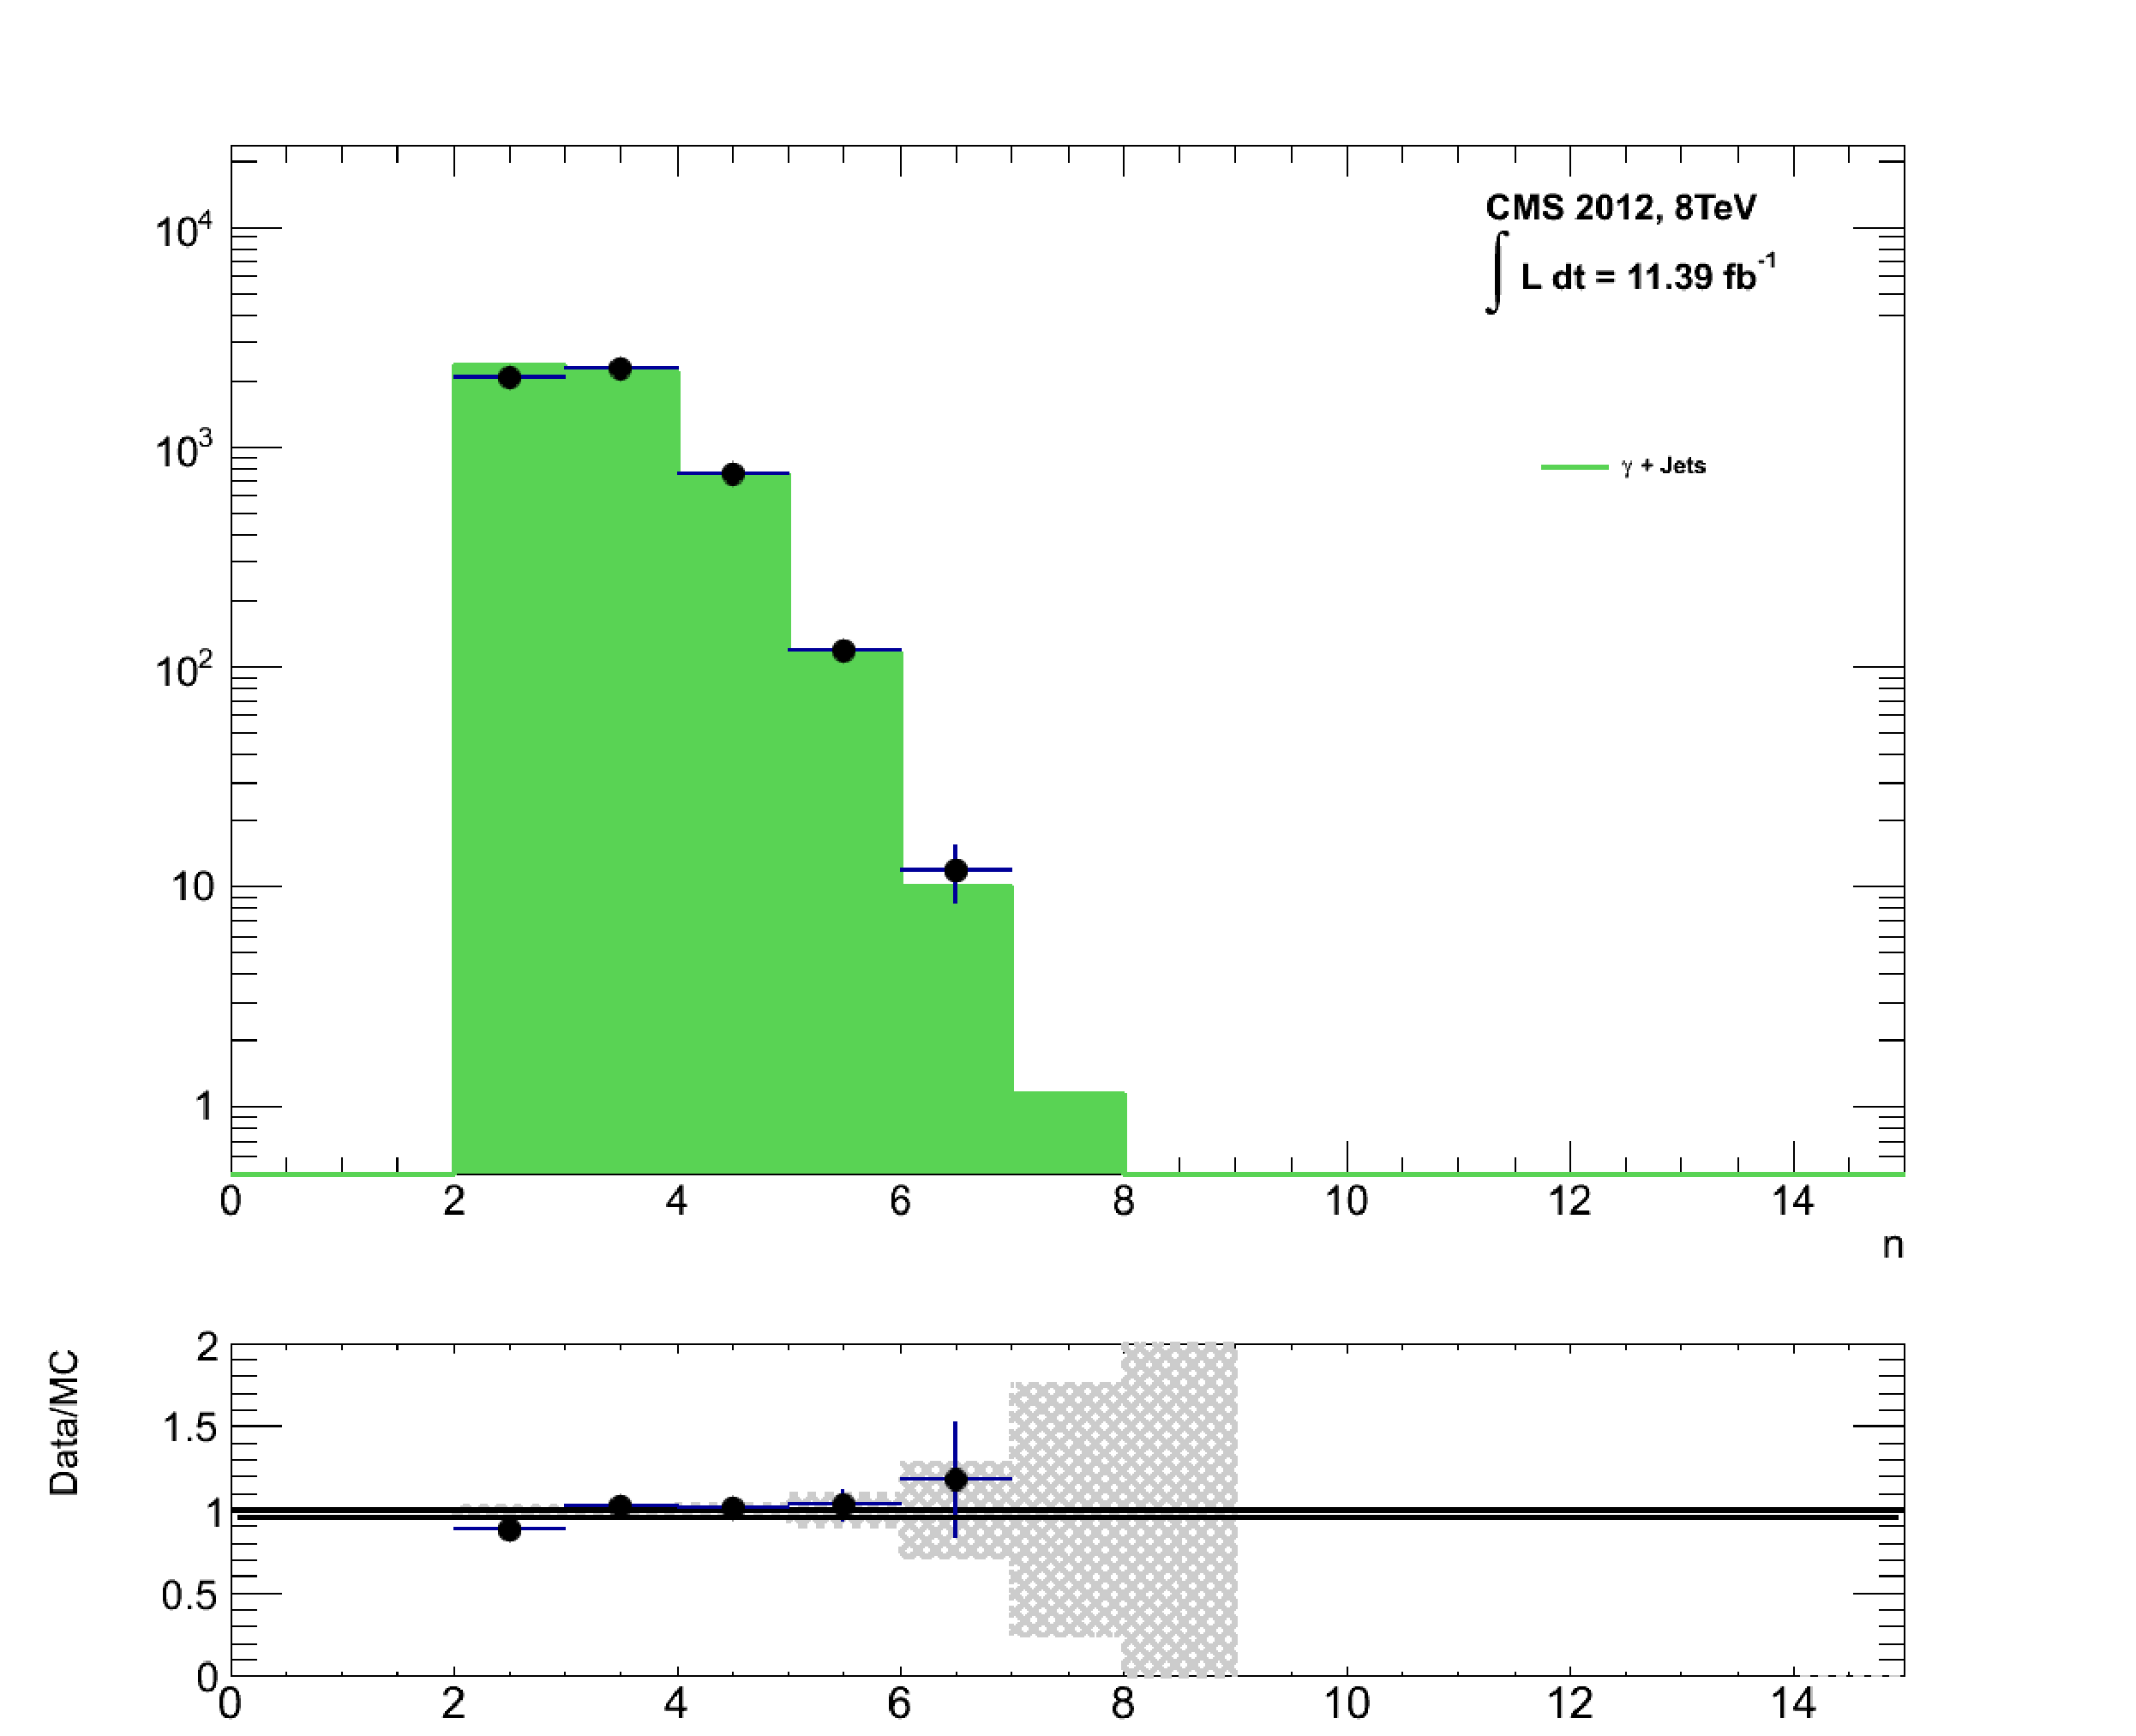
\includegraphics[width = 3.2in]{plots/photon_njet_datamc.pdf}
(d) Jet multiplicity
\end{minipage}
\captionof{figure}[Data/MC comparisons of key variables for the \gpjets selection.]{Data/MC comparisons of key variables for the \gpjets selection,following the application of selection criteria and the requirements that \theht $>$ 375 \GeV and \alphat $>$ 0.55. Bands represent the uncertainties due to the statistical size of the MC samples. No requirement is made upon the number of b-tagged jets or jet multiplicity in these distributions.}\label{fig:photonmcplots}
\end{minipage}


\end{itemize}


The selection criteria of the three control samples are defined to ensure background composition and event kinematics mirror closely the signal region. This is done in order to minimise the reliance on MC simulation to model correctly the backgrounds and event kinematics in the control and signal samples. 

However in the case of the \mupjets and \dimupjets samples, the \alphat requirement is relaxed in the selection criteria of these samples. This is made possible as contamination from QCD multi-jet events is suppressed to a negligible level by the other kinematic selection criteria within the two control samples, to select pure \ac{EWK} processes. Thus in this way, the acceptance of the two muon control samples can be significantly increased, which simultaneously improves their predictive power and further reduces the effect of any potential signal contamination. 

The modelling of the \alphat variable is probed through a dedicated set of closure tests, described in Section (\ref{subsec:sysuncertainties}), which demonstrate that the different \alphat acceptances for the control and signal samples have no significant systematic bias on the prediction.


\subsection{Estimating the QCD Background Multi-jet Background}
\label{subsec:qcdbackground}

A negligible background from QCD multi-jet events within the hadronic signal region is expected due to the selection requirement, and additional cleaning filters applied. However a conservative approach is still adopted and the likelihood model (see Section (\ref{sec:resultsintro})), is given the freedom to estimate any potential QCD multi-jet contamination. 

Any potential contamination can be identified through the variable $R_{\alphat}$, defined as the ratio of events above and below the \alphat threshold value used in the analysis. This is modelled by a \theht dependant falling exponential function which takes the form,

\begin{equation}
R_{\alphat}(\theht) =  A \exp^{-k_{QCD}\theht},
\end{equation}

where the parameters A and $k_{QCD}$ are the normalisation and exponential decay constants respectively. 

For QCD event topologies this exponential behaviour is expected as a function of \theht for several reasons. The improvement of jet energy resolution at higher \theht due to higher \pt jets leads to a narrower peaked distribution, causing $R_{\alphat}$ to fall. Similarly at higher \theht values $>$ 375 \GeV, the jet multiplicity rises slowly with \theht. As shown in Figure \ref{fig:fullalphatdistribution}, at higher jet multiplicities, the result of the combinatorics used in the determination of \alphat, also lead to a narrower \alphat distribution. 

The value of the decay constant $k_{QCD}$ is constrained via measurements within data sidebands to the signal region. This is also done to validate the falling exponential assumption for QCD multi-jet topologies. The sidebands are enriched in QCD multi-jet background and defined as regions where \alphat is relaxed or that the $R_{miss}$ cut is inverted. Figure \ref{fig:qcdcartoon} depicts the definition of these data sidebands used to constrain the value of $k_{QCD}$.

\begin{minipage}{\linewidth}
\centering
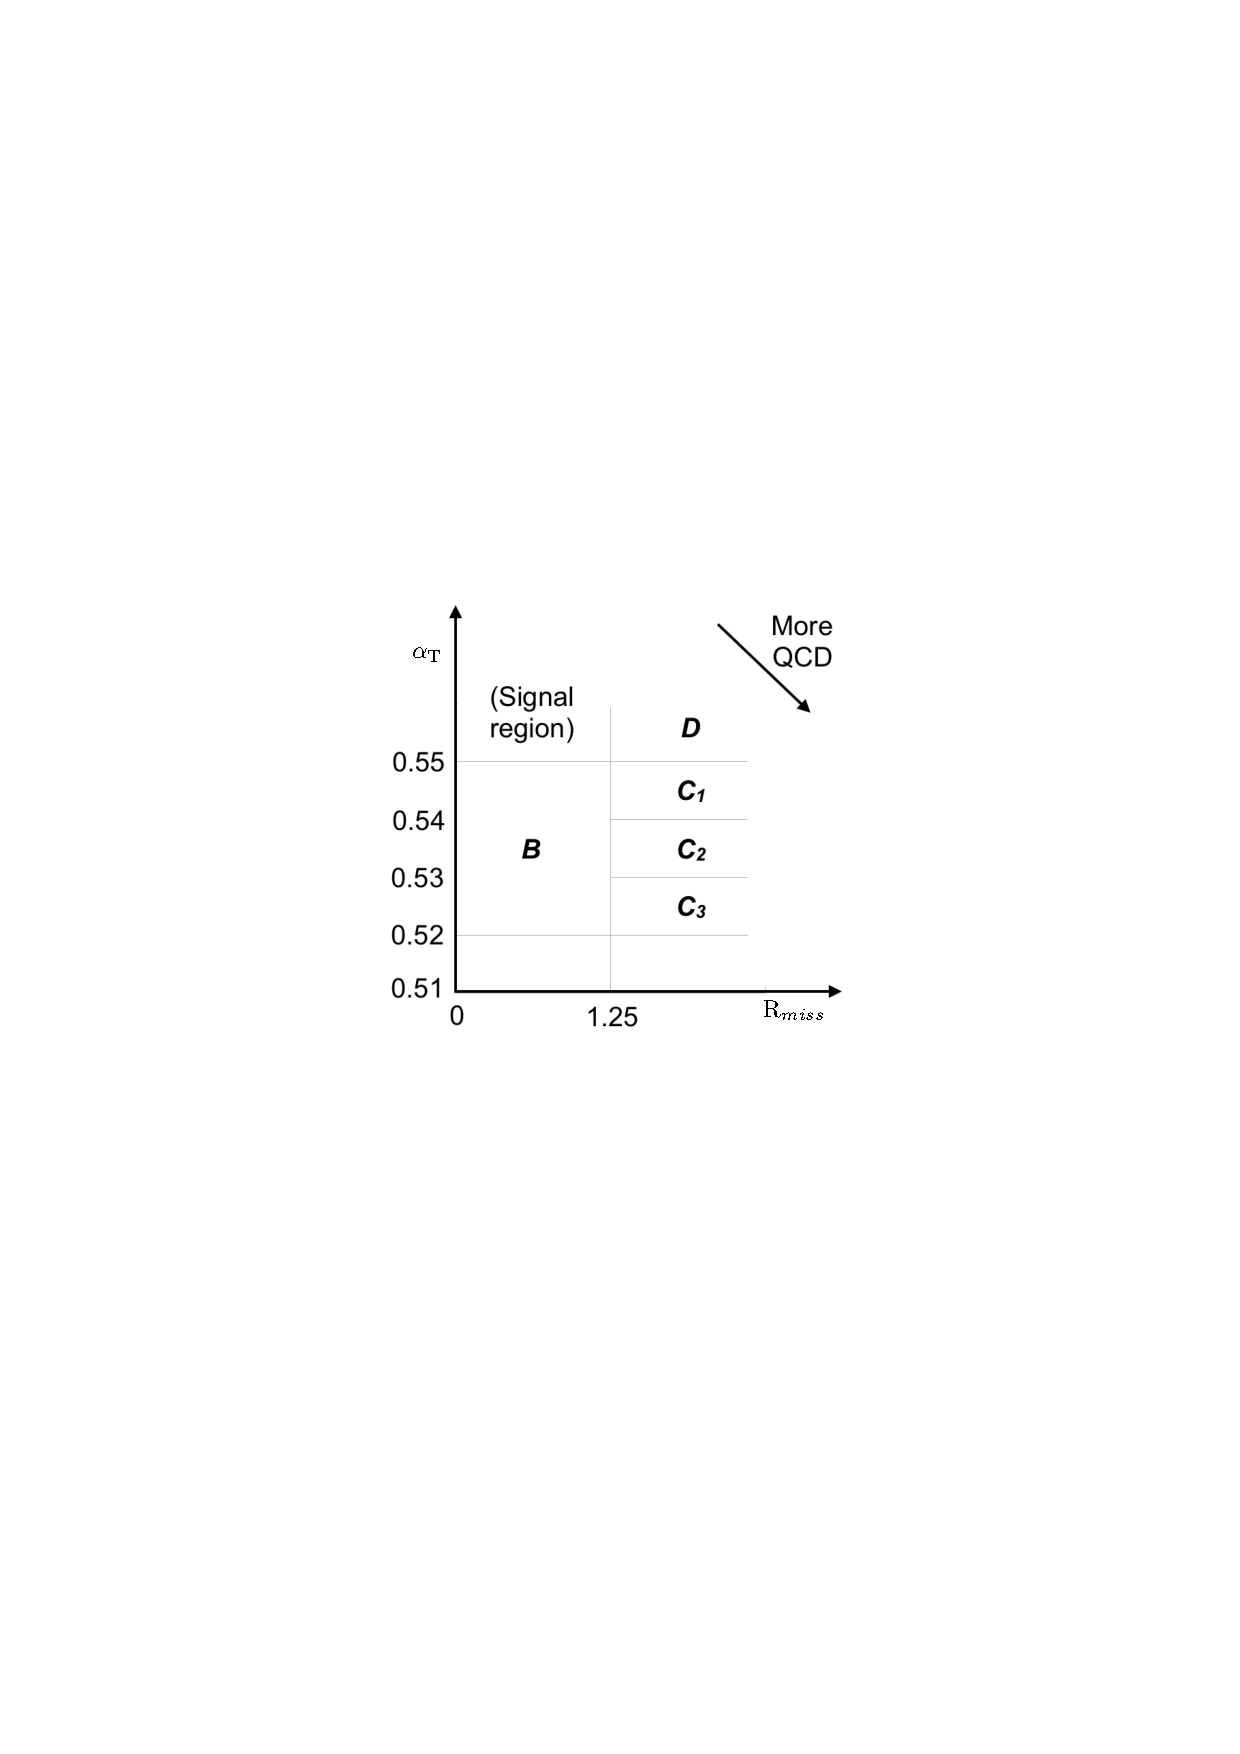
\includegraphics[width = 3.5in]{plots/qcd_cartoon.pdf}
\captionof{figure}[QCD sideband regions, used for determination of $k_{QCD}$.]{QCD sideband regions, used for determination of $k_{QCD}$.}
\label{fig:qcdcartoon}
\end{minipage}

The fits to determine the value of $k_{QCD}$ are shown in Appendix (\ref{app:kqcd}), for which the best fit value obtained from sideband region B is determined to be $k_{QCD} = 2.96 \pm 0.64 \times 10^{-2}$ \GeV$^{-1}$. 

The best fit values of the remaining three C sideband regions are used to estimate the systematic uncertainty on the central value obtained from sideband region B. The variation of these measured values is used to determine the error on the determined central value, and is calculated to be $1.31 \pm 0.26 \times 10^{-2} \GeV^{-1}$. This relative error of $\sim$ 20\% gives an estimate of the systematic uncertainty of the measurement to be applied to $k_{QCD}$.

Finally the same procedure is performed for sideband region D to establish that the value of $k_{QCD}$ extracted from a lower \alphat slice can be applied to the signal region \alphat $>$ 0.55. The likelihood fit is performed across all \theht bins within the QCD enriched region with no constraint applied to $k_{QCD}$. The resulting best fit value for $k_{QCD}$ shows good agreement between that and the weighted mean determined from the three C sidebands regions. This demonstrates that the assumption of using the central value determined from sideband region B, to provide an unbiased estimator for $k_{QCD}$ in the signal region (\alphat $>$ 0.55) is valid.

Table \ref{tab:kqcdresults}, summarises the best fit $k_{QCD}$ values determined for each of the sideband regions to the signal region.

\begin{table}[h!]
\begin{center}
\begin{tabular*}{0.5\textwidth}{@{\extracolsep{\fill}}ccc}
\cline{1-3}
Sideband region & $k_{QCD}$($\times 10^{-2} \GeV^{-1})$ & $p-$value\\ 
\cline{1-3}
B & 2.96 $\pm$ 0.64 & 0.24 \\
C$_{1}$ & 1.19 $\pm$ 0.45 & 0.93 \\
C$_{2}$ & 1.47 $\pm$ 0.37 & 0.42 \\
C$_{3}$ & 1.17 $\pm$ 0.55 & 0.98 \\
\cline{1-3}
C(weighted mean) & 1.31 $\pm$ 0.26 & - \\
D(likelihood fit) & 1.31 $\pm$ 0.09 & 0.57 \\
\cline{1-3}
\end{tabular*}
\end{center}
\caption[Best fit values for the parameters $k_{QCD}$ obtained from sideband regions B,C$_{1}$,C$_{2}$,C$_{3}$. ]{Best fit values for the parameters $k_{QCD}$ obtained from sideband regions B,C$_{1}$,C$_{2}$,C$_{3}$. The weighted mean is determined from the three measurements made within sideband region C. The maximum likelihood value of $k_{QCD}$ given by the simultaneous fit using sideband region D. Quotes errors are statistical only. }
\label{tab:kqcdresults}
\end{table}


\section{Trigger Strategy}
\label{subsec:triggerstrategy}

A cross trigger based on the quantities \theht and \alphat, labelled is used with varying thresholds across \theht bins to record the events used in the hadronic signal region. The \alphat legs of the \htalphat triggers used in the analysis are chosen to fully suppress QCD multi-jet events, whilst maintaining a sustainable trigger rate. To further maintain an acceptable rate for these analysis specific triggers, only calorimeter information is used in the reconstruction of the \theht sum, leading to the necessity for Calo jets to be used within the analysis. 

A single object prescaled \theht trigger is used to collect events for the hadronic control region described above in Section (\ref{subsec:qcdbackground}).

The performance of the \alphat and \theht triggers used to collect data for the signal and hadronic control region is measured with respect to a reference sample collected using the muon system. This allows measurement of both the Level 1 seed and higher level triggers simultaneously, as the reference sample is collected independent of any jet requirements. 

The selection for the trigger efficiency measurement is identical to that described in Section (\ref{subsec:eventselection}), with the requirement of exactly one well identified muon with \pt $>$ 30 \GeV which is subsequently ignored.  

The efficiencies measure for the \htalphat triggers in bins indiviual \theht and \alphat legs, is summarised in Table \ref{tab:trigeffs}.

\begin{table}[h!]
\begin{center}
\begin{tabular*}{0.5\textwidth}{@{\extracolsep{\fill}}ccc}
\cline{1-3}
\theht range (\GeV) & $\epsilon$ on \theht leg (\%) & $\epsilon$ on \alphat leg (\%) \\ 
\cline{1-3}
275-325 & $87.7^{+1.9}_{-1.9}$ & $82.8^{+1.0}_{-1.1}$ \\
325-375 & 90.6$^{+2.9}_{-2.9}$ & 95.9$^{+0.7}_{-0.9}$ \\
375-475 & 95.7$^{+0.1}_{-0.1}$ & 98.5$^{+0.5}_{-0.9}$ \\
475-$\infty$ & 100.0$^{+0.0}_{-0.0}$ & 100.0$^{+0.0}_{-4.8}$ \\
\cline{1-3}
\end{tabular*}
\end{center}
\caption[Measured efficiencies of the \theht and \alphat legs of the HT and \htalphat triggers in independent analysis bins.]{Measured efficiencies of the \theht and \alphat legs of the HT and \htalphat triggers in independent analysis bins. The product of the two legs gives the total efficiency of the trigger in a given offline \theht bin.}
\label{tab:trigeffs}
\end{table}

Data for the control samples of the analysis, detailed in Section (\ref{subsec:controlsampledefinition}), are collected using single object photon trigger for the \gpjets sample, and a single object muon trigger for both the \mupjets and \dimupjets control samples. The photon trigger is measured to be full efficient for the threshold $\pt^{photon} > 150 \GeV$, whilst the single muon efficiency satisfying $\pt^{muon} > 30 \GeV$ is measured to have an efficiency of (88$\pm$2)\% that is independent of \theht. In the case of the \dimupjets control sample, the efficiency is measured to be (95$\pm$2)\% for the lowest \theht bin, rising to (98$\pm$2)\% for the highest \theht bin.

\section{Measuring MC normalisation factors via \theht sidebands}
\label{subsec:mckfactors}

The theoretical cross sections of different \ac{SM} processes at \acf{NNLO} and the number of MC simulated events generated for that particular process, is typically used to determine the appropriate normalisation for a MC sample. However within the particular high-\theht and high-\met corners of kinematic phase space probed within this search, the theoretical cross sections for various processes are far less well understood. 

To mitigate the problem of theoretical uncertainties and arbitrary choices of cross sections, the normalisation of MC samples used in the analysis are determined through the use data sidebands. The sidebands are used to calculated sample specific correct factors (k-factors) that are appropriate for the \theht-\met phase space coverd by this analysis. 

They are defined within the \mupjets and \dimupjets control sample, by the region 200$<$ \theht$<$275, using the same jet \pt thresholds as the adjacent first analysis bin. Individual \ac{EWK} processes are isolated within each of these control samples via requirements on jet multiplicity and the requirement on b-tags, summarised in Table \ref{tab:mckfactors}. The purity of the samples are typically $>$ 90\% with any residual contamination corrected for. The resultant k-factor for each process is determined by then taking ratio of the data yield over the MC expectation in the sideband. Subsequently these k-factors are then applied to the processes within the phase space of the analysis.

 \begin{table}[h!]
\begin{center}
\begin{tabular*}{0.95\textwidth}{@{\extracolsep{\fill}}llccc}
\cline{1-5}
Process & Selection & Observation & MC expectation & k-factor \\
\cline{1-5}
W + jets & \mupjets, n$_{b}$=0, n$_{jet}$ = 2,3 &26950 & 29993.2 $\pm$ 650.1 & 0.90 $\pm$ 0.02 \\
$Z \rightarrow \mu\mu$ + jets & \dimupjets, n$_{b}$=0, n$_{jet}$ = 2,3 & 3141 & 3402.0 $\pm$ 43.9 & 0.92 $\pm$ 0.02 \\
\ttbar & \mupjets, n$_{b}$=2, n$_{jet}$ = $\geq$4 & 2190 & 1967.8 $\pm$ 25.1 & 1.11 $\pm$ 0.02 \\
\cline{1-5}
\end{tabular*}
\end{center}
\caption[k-factors calculated for different \ac{EWK} processes.]{k-factors calculated for different \ac{EWK} processes. All k-factors are derived relative to theoretical cross sections calculated in \ac{NNLO}. The k-factors measured for the Z$\rightarrow \mu\mu$ + jets processes, are also applied to the \zinv + jets and \gpjets MC samples.}\label{tab:mckfactors}
\end{table}


\section{Determining MC Yields With Higher Statistical Precision}
\label{subsec:backgroundestimation}

Reconstructing events from \ac{EWK} processes with many b-tagged jets ($\geq$3),\nbreco  ,is largely driven by the mis-tagging of light jets within the event. This is clear when considering the main \ac{EWK} backgrounds in the analysis, such as \ttbar + jets events, which typically contain two b-flavoured jets from the decay of the top quarks, whilst W + jets and Z$\rightarrow \mu\mu$ + jets events will typically contain no b-flavoured jets.

When the expectation for the number of \nbreco is taken directly from simulation, the statistical uncertainty at large b-tag multiplicities becomes relatively large. In order to reduce this uncertainty one approach is to use the information encoded throughout all events in the simulation sample, to measure each of the four ingredients:

\begin{enumerate}
\item the b-tagging efficiency in the event selection,
\item the charm-tagging efficiency in the event selection
\item the mis-tagging rate in the event selection,
\item the underlying flavour distribution of the jets in the events,
\end{enumerate}

 that determine the \nbreco distribution of the process being measured. This method allows the determination of higher b-tag multiplicities to a higher degree of accuracy reducing the statical uncertainties of the MC which enter into the \ac{TF}'s. For the discussion that follows, these predictions are determined on average (i.e not on an event-by-event basis), and is known as the formula method.

\subsection{ The formula method}
\label{subsec:formulamethod}

The assigning of jet flavours to reconstruction level jets in simulation is achieved via an algorithmic method defined as:

\begin{itemize}
\item Try to find the parton that most likely determines the properties of the jet and assign that flavour as true flavour,
\item Here, the ``final state'' partons (after showering, radiation) are analysed (also within $\Delta R <$ 0.3 of reconstructed jet cone),
\item Jets from radiation are matched with full efficiency,
\item If there is a b/c flavoured parton within the jet cone: label as b/c flavoured jet,
\item Otherwise: assign flavour of the hardest parton.
\end{itemize}

Within each individual MC process and each \theht-$n_{jet}$ bin in the analysis, the \nbreco distribution is constructed in the following way:

 Let \nbcq represent the yield in simulation of events with \textit{b} underlying b-quarks, \textit{c} underlying c-quarks and \textit{q} underlying light quarks which are matched to reconstructed jets. Light quarks are defined as those which originate from a \textit{u},\textit{d},\textit{s},\textit{g} and $\tau$ jets which are grouped together having similar mis-tagging rates.  Similarly defining \eff, \ceff and \textit{m}, which represent the measured b-tagging,c-tagging and mis-tagging efficiency averaged over all the jets within that particular analysis bin. 
 
 Using this information the expected number of jets which have been b-tagged can be analytically calculated using the formula :

\begin{align}
\label{eq:btagformula}
N(n_{b}) =& \sum_{n_{b}^{gen}+n_{c}^{gen}+n_{q}^{gen} = n_{jet}} \quad \sum_{n_{b}^{tag}+n_{c}^{tag}+n_{q}^{tag} = n_{b}} \nbcq \times \probb \times \nonumber \\
& \probc \times \probl,
\end{align}

with N(n$_{b}$) representing the event yield where $n_{b}$ jets have been b-tagged, $n_{b}^{tag}$, $n_{c}^{tag}$ and $n_{q}^{tag}$ represent the number of times that a particular jet flavour results in a b-tagged jet, and \probb,\probc and \probl represent the binomial probabilities for that to happen. 

This approach ultimately results in a more precise \nbreco distribution prediction as information from throughout the entire MC sample is used to estimate the high $n_{b}^{reco}$ bins.

\subsection{Establishing proof of principle}
\label{subsec:formulamethodsanity}

In order to validate the procedure, the predictions obtained from the formula method summarised in Eq (\ref{eq:btagformula}), are compared directly to those obtained directly from simulation. These results for the \mupjets control sample are summarised in Table \ref{tab:sanitycheck}, for the 0,1,2 and 3 $n_{b}^{reco}$ bins.  

 \begin{table}[h!]
\begin{center}
\begin{tabular*}{0.95\textwidth}{@{\extracolsep{\fill}}llccc}
\cline{1-5}
Process & Selection & Observation & MC expectation & k-factor \\
\cline{1-5}
\end{tabular*}
\end{center}
\caption[place holder]{place holder}\label{tab:sanitycheck}
\end{table}

\subsection{Correcting Measured Efficiencies In Simulation To Data}
\label{subsec:formulamethodsf}

As detailed in Section (\ref{subsec:cmsobjects-btagging}), it is necessary for certain \pt and $\eta$ dependant corrections, to be applied to both the b-tagging efficiency and mis-tagging rates in order correct the efficiencies from simulation to the distributions seen in data. These corrections are factored in�.

Show plot of before and after correction to btag/mistag rate.


These corrections come with uncertainties�..

show plot of effect of scaling correction factor up and down.
2
\section{Systematic Uncertainties On Transfer Factors}
\label{subsec:sysuncertainties}

Since the \ac{TF}'s used to establish the background prediction are obtained from simulation, an appropriate systematic uncertainty is assigned to each factor to account for theoretical uncertainties \cite{Bern:2011pa} and limitations in the simulation modelling of event kinematics and instrumental effects. 

The magnitudes of these systematic uncertainties are established through a set of data driven method, in which the three independent control samples of the analysis (\mupjets, \dimupjets, \gpjets) are used to in a series of closure tests. The yields from one of these control samples, along with the corresponding \ac{TF} obtained from simulation, are used to predict the yields in another control sample, using the same method of establishing a background prediction for the signal region as described in Section (\ref{subsec:controlsampledefinition}).

The level of agreement between the predicted and observed yields is expressed as the ratio 

\begin{equation}
\label{eq:closuretests}
\frac{(N_{obs}-N_{pred})}{N_{pred}},
\end{equation}

while considering only the statistical uncertainties on $N_{pred}$, the prediction, and $N_{obs}$, the observation. No systematic uncertainty is assigned to the prediction, and resultantly the level of closure is defined by the statistical significance of a deviation from the ratio from zero.

This ratio is measured for each \theht bin in the analysis, allowing these closure tests to be sensitive to both the presence of any significant biases or any possible \theht dependence on the level of closure.

Eight sets of closure tests are defined between the three data control samples, conducted independently between the two jet multiplicity (2 $\leq n_{jets} \leq 3$, $n_{jet} \geq 4$ ) bins. Each of these tests are specifically chosen to probe each of the different key ingredients of the simulation modelling that can affect the background prediction.

Each of the different modelling components and the relevant closure tests are described below :

\begin{itemize}

\item[] \textbf{\alphat modelling}

The modelling of the \alphat distribution in genuine \met events is probed with the \mupjets control sample. This test is important to verify the approach of remove the \alphat $>$ 0.55 requirement from the \mupjets and \dimupjets samples to increase the precision of the background prediction. The test uses the \mupjets sample without an \alphat cut to make a prediction into the \mupjets sample defined with the requirement  \alphat $>$ 0.55.

\item[] \textbf{Background admixture}

The sensitivity of the translation factors to the relative admixture of events from $W +$ jets and \ttbar processes is probed by two closure tests. These tests represent an extremely conservative approach as the admixture of the background remains similar between the \mupjets sample and the signal region, contrary to the defined closure tests which make predictions between two very different admixtures of $W +$ jets and \ttbar events.  

Within the \mupjets sample, a W boson enriched sub-sample ($n_{b} =$ 0) is used to predict yields in a \ttbar enriched sub-sample ($n_{b} =$ 1). Similarly the \\tbar enriched sub-sample ($n_{b} =$1) is also used to predict yields for a further enriched \ttbar sub-sample ($n_{b} =$ 2). 

Similarly a further closure test probes the relative contribution of $Z +$ jets to $W +$jets and \ttbar events, through the use of the \mupjets sample to predict yields for the \dimupjets control sample. This closure test, also at some level probes the muon trigger and reconstruction efficiencies, given that exactly one and two muons are required by the different selections.
 
\item[] \textbf{Consistency between control samples}

An important consistency check between the \dimupjets jets and \gpjets, which are both used in the prediction of the \zinv in the signal region, is measured by using the \gpjets sample to predict yields for the \dimupjets control sample.

\item[]\textbf{Modelling of jet multiplicity}

The simulation modelling of the jet multiplicity within each control sample is important due to the exclusive jet multiplicity binning within the analysis. This is probed via the use of each of the three control samples to independently predict from the lower jet multiplicity category $2 \leq n_{jet} \leq 3$, to the high jet category $\geq 4$. 

For the case of the \mupjets and \dimupjets control samples this test this is also a further probe of the admixture between $W +$ jets/$Z +$ jets and \ttbar. Once again these three tests represent a conservative approach, as background predictions are always made from the same jet multiplicity bin, whereas the closure tests translate between these bins.
 
\end{itemize}

To test for the assumption that no \theht dependences exist within the background predictions of the analysis, the first five closure tests defined above are taken, with zeroeth and first order polynomial fits are applied to each. This is summarised in Table \ref{tab:closuretestfitslow} and Table \ref{tab:closuretestfitshigh} which show the results for both the 2 $\leq n_{jet} \leq 3$ and $\geq 4$ jet multiplicity bins respectively.

 \begin{table}[h!]
\begin{center}
\begin{tabular*}{0.95\textwidth}{@{\extracolsep{\fill}}ll|cc|cc}
\cline{1-6}
& & \multicolumn{2}{c|}{\footnotesize{Constant fit}} & \multicolumn{2}{c}{\footnotesize{Linear fit}} \\ 
\footnotesize{Closure test} & \footnotesize{Symbol} & \footnotesize{Best fit value} & \footnotesize{p-value} & \footnotesize{Slope (10$^{-4}$)} & \footnotesize{p-value} \\
\cline{1-6}
\footnotesize{\alphat $< 0.55 \rightarrow \alphat > 0.55$ (\mupjets)} & \footnotesize{Circle} & $-0.06 \pm 0.02$ & 0.93 & $-1.3 \pm 2.2$ & 0.91 \\ 
\footnotesize{0 b-jets $\rightarrow$ 1 b-jet (\mupjets)} & \footnotesize{Square} & $ \footnotesize{\quad}0.07 \pm 0.02$ & 0.98 & $-1.6 \pm 1.6$ & 1.00 \\ 
\footnotesize{1 b-jets $\rightarrow$ 2 b-jet (\mupjets)} & \footnotesize{Triangle} & $ -0.07 \pm 0.03$ & 0.76 & $-2.7 \pm 3.0$ & 0.76 \\ 
\footnotesize{\mupjets $\rightarrow$ \dimupjets} & \footnotesize{Cross} & $ \footnotesize{\quad}0.10 \pm 0.03$ & 0.58 & $-1.1 \pm 2.3$ & 0.49 \\ 
\footnotesize{\dimupjets $\rightarrow$ \gpjets} & \footnotesize{Star} & $ -0.06 \pm 0.04$ & 0.31 & $\footnotesize{\quad}4.2 \pm 4.3$ & 0.29 \\ \cline{1-6}
\end{tabular*}
\end{center}
\caption[A summary of the results obtained from fits of zeroeth order polynomials (i.e. a constant) to five sets of closure tests performed in the 2 $\leq n_{jet} \leq$ 3 bin]{A summary of the results obtained from fits of zeroeth order polynomials (i.e. a constant) to five sets of closure tests performed in the 2 $\leq n_{jet} \leq$ 3 bin. The final two columns show the best fit value for the slope obtained when performing a linear fit and the p-value for the linear fit.}\label{tab:closuretestfitslow}
\end{table}

 \begin{table}[h!]
\begin{center}
\begin{tabular*}{0.95\textwidth}{@{\extracolsep{\fill}}ll|cc|cc}
\cline{1-6}
& & \multicolumn{2}{c|}{\footnotesize{Constant fit}} & \multicolumn{2}{c}{\footnotesize{Linear fit}} \\ 
\footnotesize{Closure test} & \footnotesize{Symbol} & \footnotesize{Best fit value} & \footnotesize{p-value} & \footnotesize{Slope (10$^{-4}$)} & \footnotesize{p-value} \\
\cline{1-6}
\footnotesize{\alphat $< 0.55 \rightarrow \alphat > 0.55$ (\mupjets)} & \footnotesize{Circle} & $-0.05 \pm 0.03$ & 0.21 &  $\footnotesize{\quad}3.0 \pm 2.9$ & 0.21 \\ 
\footnotesize{0 b-jets $\rightarrow$ 1 b-jet (\mupjets)} & \footnotesize{Square} & $ -0.03 \pm 0.03$ & 0.55 & $-1.0 \pm 1.9$ & 0.47 \\ 
\footnotesize{1 b-jets $\rightarrow$ 2 b-jet (\mupjets)} & \footnotesize{Triangle} & $ -0.02 \pm 0.03$ & 0.39 & $ \footnotesize{\quad}1.1 \pm 2.2$ & 0.31 \\ 
\footnotesize{\mupjets $\rightarrow$ \dimupjets} & \footnotesize{Cross} & $  \footnotesize{\quad}0.08 \pm 0.07$ & 0.08 &  $\footnotesize{\quad}4.8 \pm 4.3$ & 0.07 \\ 
\footnotesize{\dimupjets $\rightarrow$ \gpjets} & \footnotesize{Star} & $ -0.03 \pm 0.10$ & 0.72 & $-4.0 \pm 7.0$ & 0.64 \\ \cline{1-6}
\end{tabular*}
\end{center}
\caption[A summary of the results obtained from fits of zeroeth order polynomials (i.e. a constant) to five sets of closure tests performed in the $n_{jet} \geq$ 4 bin]{A summary of the results obtained from fits of zeroeth order polynomials (i.e. a constant) to five sets of closure tests performed in the $ n_{jet} \geq$ q bin. The final two columns show the best fit value for the slope obtained when performing a linear fit and the p-value for the linear fit.}\label{tab:closuretestfitshigh}
\end{table}

Table \ref{tab:closuretestfitsall} shows the same fits applied to the three closure tests that probe the modelling between the different $n_{jet}$ bins. The best fit value and its uncertainty is listed for each set of closure tests in all three tables, along with the p-value of the constant and linear fits applied. 

 \begin{table}[h!]
\begin{center}
\begin{tabular*}{0.95\textwidth}{@{\extracolsep{\fill}}ll|cc|cc}
\cline{1-6}
& & \multicolumn{2}{c|}{\footnotesize{Constant fit}} & \multicolumn{2}{c}{\footnotesize{Linear fit}} \\ 
\footnotesize{Closure test} & \footnotesize{Symbol} & \footnotesize{Best fit value} & \footnotesize{p-value} & \footnotesize{Slope (10$^{-4}$)} & \footnotesize{p-value} \\
\cline{1-6}
\footnotesize{\mupjets} & \footnotesize{Inverted triangle} & $-0.03 \pm 0.02$ & 0.02 & $\footnotesize{\quad}0.0 \pm 1.0$ & 0.01 \\ 
\footnotesize{\mupjets (outlier removed)} & \footnotesize{Inverted triangle} & $-0.04 \pm 0.01$ & 0.42 & $-1.4 \pm 1.1$ & 0.49 \\ 
\footnotesize{\gpjets} & \footnotesize{Diamond} & $  \footnotesize{\quad}0.12 \pm 0.05$ & 0.79 & $\footnotesize{\quad}6.0 \pm 4.7$ & 0.94 \\ 
\footnotesize{\dimupjets} & \footnotesize{Asterisk} & $ -0.04 \pm 0.07$ & 0.20 &  $\footnotesize{\quad}4.9 \pm 4.4$ & 0.20 \\ 
\cline{1-6}
\end{tabular*}
\end{center}
\caption[A summary of the results obtained from fits of zeroeth order polynomials (i.e. a constant) to five sets of closure tests performed in the 2 $\leq$ njet $\leq$ 3 bin]{A summary of the results obtained from fits of zeroeth order polynomials (i.e. a constant) to five sets of closure tests performed in the 2 $\leq$ njet $\leq$ 3 bin. The final two columns show the best fit value for the slope obtained when performing a linear fit and the p-value for the linear fit.}\label{tab:closuretestfitsall}
\end{table}

The best fit value for the constant parameter is indicative of the level of closure, averaged across the full range of \theht bins in the analysis, and the p-value an indicator of any significant dependence on \theht within the closure tests. The best fit values of all the tests are either statistically compatible with zero bias (i.e, less than $2\sigma$ from zero) or at the level of 10\% or less, with the exception of one closure test discussed below. 

Within Table \ref{tab:closuretestfitsall}, there exists one test that does not satisfy the above statement, which is the $2 \leq n_{jet} \leq 3 \rightarrow n_{jet} \geq 4$ test using the \mupjets control sample. The low p-value can be largely attributed to an outlier in the 675 $<$ \theht $<$ 775 \GeV bin, rather than any significant trend in \theht. Removing this single outlier from the constant fit performed, gives a best fit value of $-0.04 \pm 0.01$, $\chi^{2} /$ d.o.f = 6.07/6. and a p-value of 0.42. These modified fit results are included within Table \ref{tab:closuretestfitsall} .

In addition the best fit values for the slope terms of the linear fits in all three tables are of the order $10^{-4}$, which corresponds to a percent level change per 100 \GeV. However in all cases, the best fit values are fully compatible with zero (within 1$\sigma$) once again with the exception detailed above, indicating that the level of closure is \theht independent.




\section{Searches For Natural SUSY With B-tag Templates.}
\label{sec:templatemethod}

Btag Templates blah blah

